% Created 2015-11-04 Wed 18:12
\documentclass[9pt]{beamer}
\usepackage[utf8]{inputenc}
\usepackage[T1]{fontenc}
\usepackage{fixltx2e}
\usepackage{graphicx}
\usepackage{longtable}
\usepackage{float}
\usepackage{wrapfig}
\usepackage{soul}
\usepackage{textcomp}
\usepackage{marvosym}
\usepackage{wasysym}
\usepackage{latexsym}
\usepackage{amssymb}
\usepackage{hyperref}
\tolerance=1000
\mode<beamer>{\usetheme{Warsaw}}
\mode<beamer>{\setbeamertemplate{blocks}[rounded][shadow=false]}
\mode<beamer>{\addtobeamertemplate{block begin}{\pgfsetfillopacity{0.8}}{\pgfsetfillopacity{1}}}
\mode<beamer>{\setbeamercolor{structure}{fg=orange}}
\mode<beamer>{\setbeamercovered{transparent}}
\AtBeginSection[]{\begin{frame}<beamer>\frametitle{Topic}\tableofcontents[currentsection]\end{frame}}
\usepackage{subcaption}
\usepackage{multimedia}
\usepackage{tikz}
\usepackage{subfigure,subfigmat}
\usepackage{threeparttable}
\usetikzlibrary{shapes,arrows,shadows}
\usepackage{bm, amssymb, amsmath, array, pdfpages}
\newcommand{\bv}[1]{\mathbf{#1}}
\newcommand{\diff}[2]{\frac{\partial #1}{\partial #2}}
\newcommand{\beq}[0]{\begin{equation}}
\newcommand{\eeq}[0]{\end{equation}}
\newcommand{\beqa}[0]{\begin{eqnarray}}
\newcommand{\eeqa}[0]{\end{eqnarray}}
\newcommand{\beqq}[0]{\begin{equation*}}
\newcommand{\eeqq}[0]{\end{equation*}}
\newcommand{\bs}[1]{\boldsymbol{#1}}
\newcommand{\ip}[2]{\langle #1, #2\rangle}
\providecommand{\alert}[1]{\textbf{#1}}

\title{Low-Dimensional Modeling and Uncertainty Quantification for Airfoil Icing}
\author{Anthony DeGennaro \newline Clarence W. Rowley III \newline Luigi Martinelli \newline Princeton University}
\date{FAA JUP Summer 2015 Quarterly Meeting \\ Athens, OH \\ August 2015}
\hypersetup{
  pdfkeywords={},
  pdfsubject={},
  pdfcreator={Emacs Org-mode version 7.9.3f}}

\begin{document}

\maketitle

\begin{frame}
\frametitle{Outline}
\setcounter{tocdepth}{3}
\tableofcontents
\end{frame}



% Define my settings

\graphicspath{{Figures/}}
% Add Princeton shield logo
\addtobeamertemplate{frametitle}{}{%
\begin{tikzpicture}[remember picture,overlay]
\node[anchor=north east,yshift=2pt] at (current page.north east) {
\includegraphics[height=0.7cm]{Shield}};
\end{tikzpicture}}
%


\institute{Princeton University}


\section{Motivation/Background}
\label{sec-1}
\begin{frame}
\frametitle{Introduction}
\label{sec-1-1}

\textbf{Motivation}
\begin{itemize}
\item Wing icing is a serious issue for pilots
\begin{itemize}
\item Massive flow separation, lower lift + higher drag
\item Unpredictable stall
\end{itemize}
\item Wing ice shapes exhibit wide variation, sensitivity to physical
  parameters
\begin{itemize}
\item Complex physics (coupled airflow-thermodynamics)
\item Uncertainty in physical parameters
\end{itemize}
\end{itemize}
\textbf{Research Goals}
\begin{itemize}
\item How can observed variations in ice shape be modeled
  efficiently with a low number of parameters?
\item How does uncertainty in the ice shape create uncertainty in
  aerodynamic performance?
\end{itemize}
\end{frame}
\begin{frame}
\frametitle{Experimental/Computational Variation in Ice Shape}
\label{sec-1-2}


\vspace*{-0.5cm}\begin{figure}
  \begin{subfigmatrix}{2}
      \subfigure[Habashi, 2006]{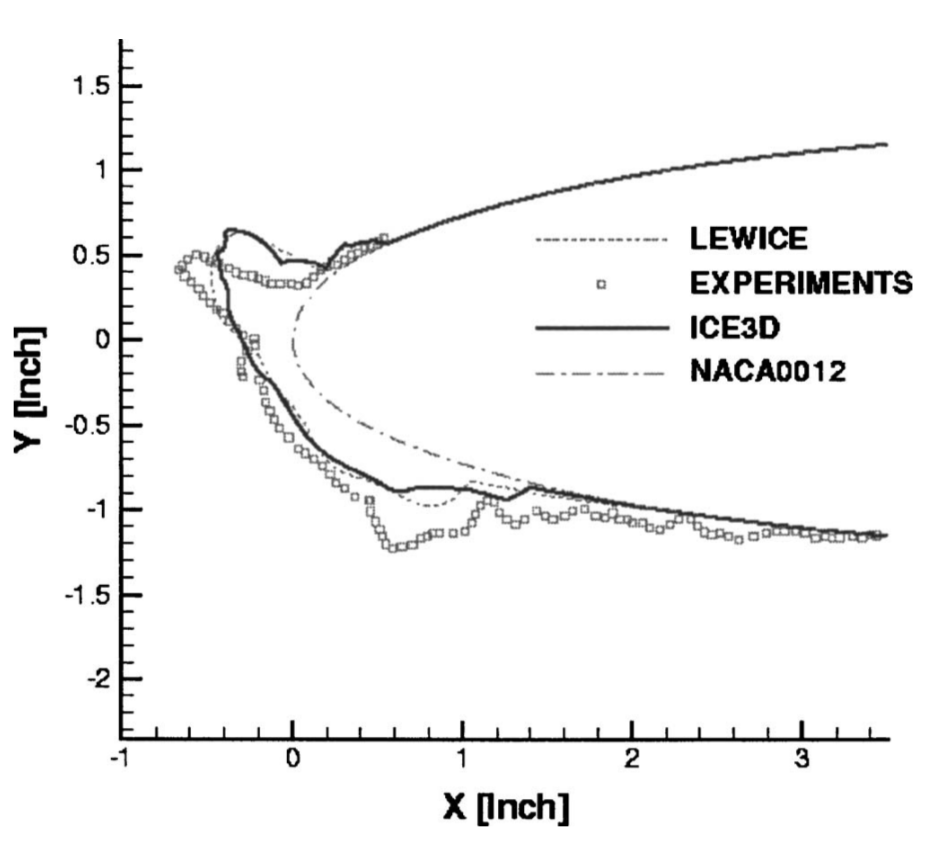
\includegraphics[width=0.4\textwidth]{Habashi2006ShapeVariation}}
      \subfigure[Wright, 2004]{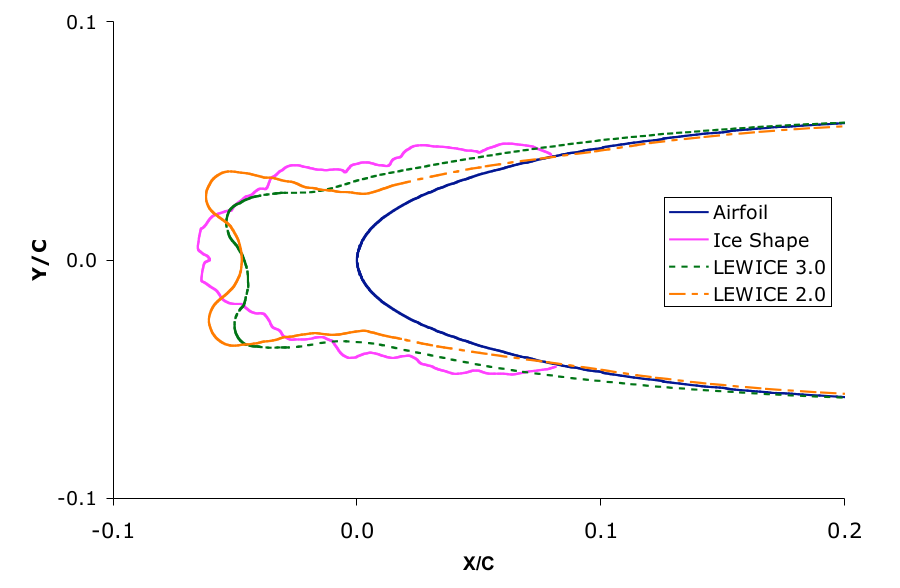
\includegraphics[width=0.4\textwidth]{Wright2004ShapeVariation}}
  \end{subfigmatrix}
\end{figure}

\begin{itemize}
\item Wide variation in experimental/computational ice shapes\footnote{Beaugendre H., Morency M., and Habashi W.G. \emph{Development of a Second Generation in-Flight Icing Simulation Code}. Journal of
Fluids Engineering, ASME, 2006.
 }\textsuperscript{,}\,\footnote{Wright W. and Potapczuk, M.G. \emph{Semi-Empirical Modeling of SLD Physics}, AIAA 2004-412. 42$^{nd}$ AIAA Aerospace Sciences
Meeting, Reno, NV, 2004.
 }
\item Suggests sensitivity to perturbations in underlying physical
  processes
\item \emph{UQ approach:} parameterize the shape variation and study its
  effects on aerodynamics
\end{itemize}
\end{frame}
\begin{frame}
\frametitle{Relation to Previous Work}
\label{sec-1-3}


\begin{columns}[c]
  \column{0.33\textwidth}
    \centering
    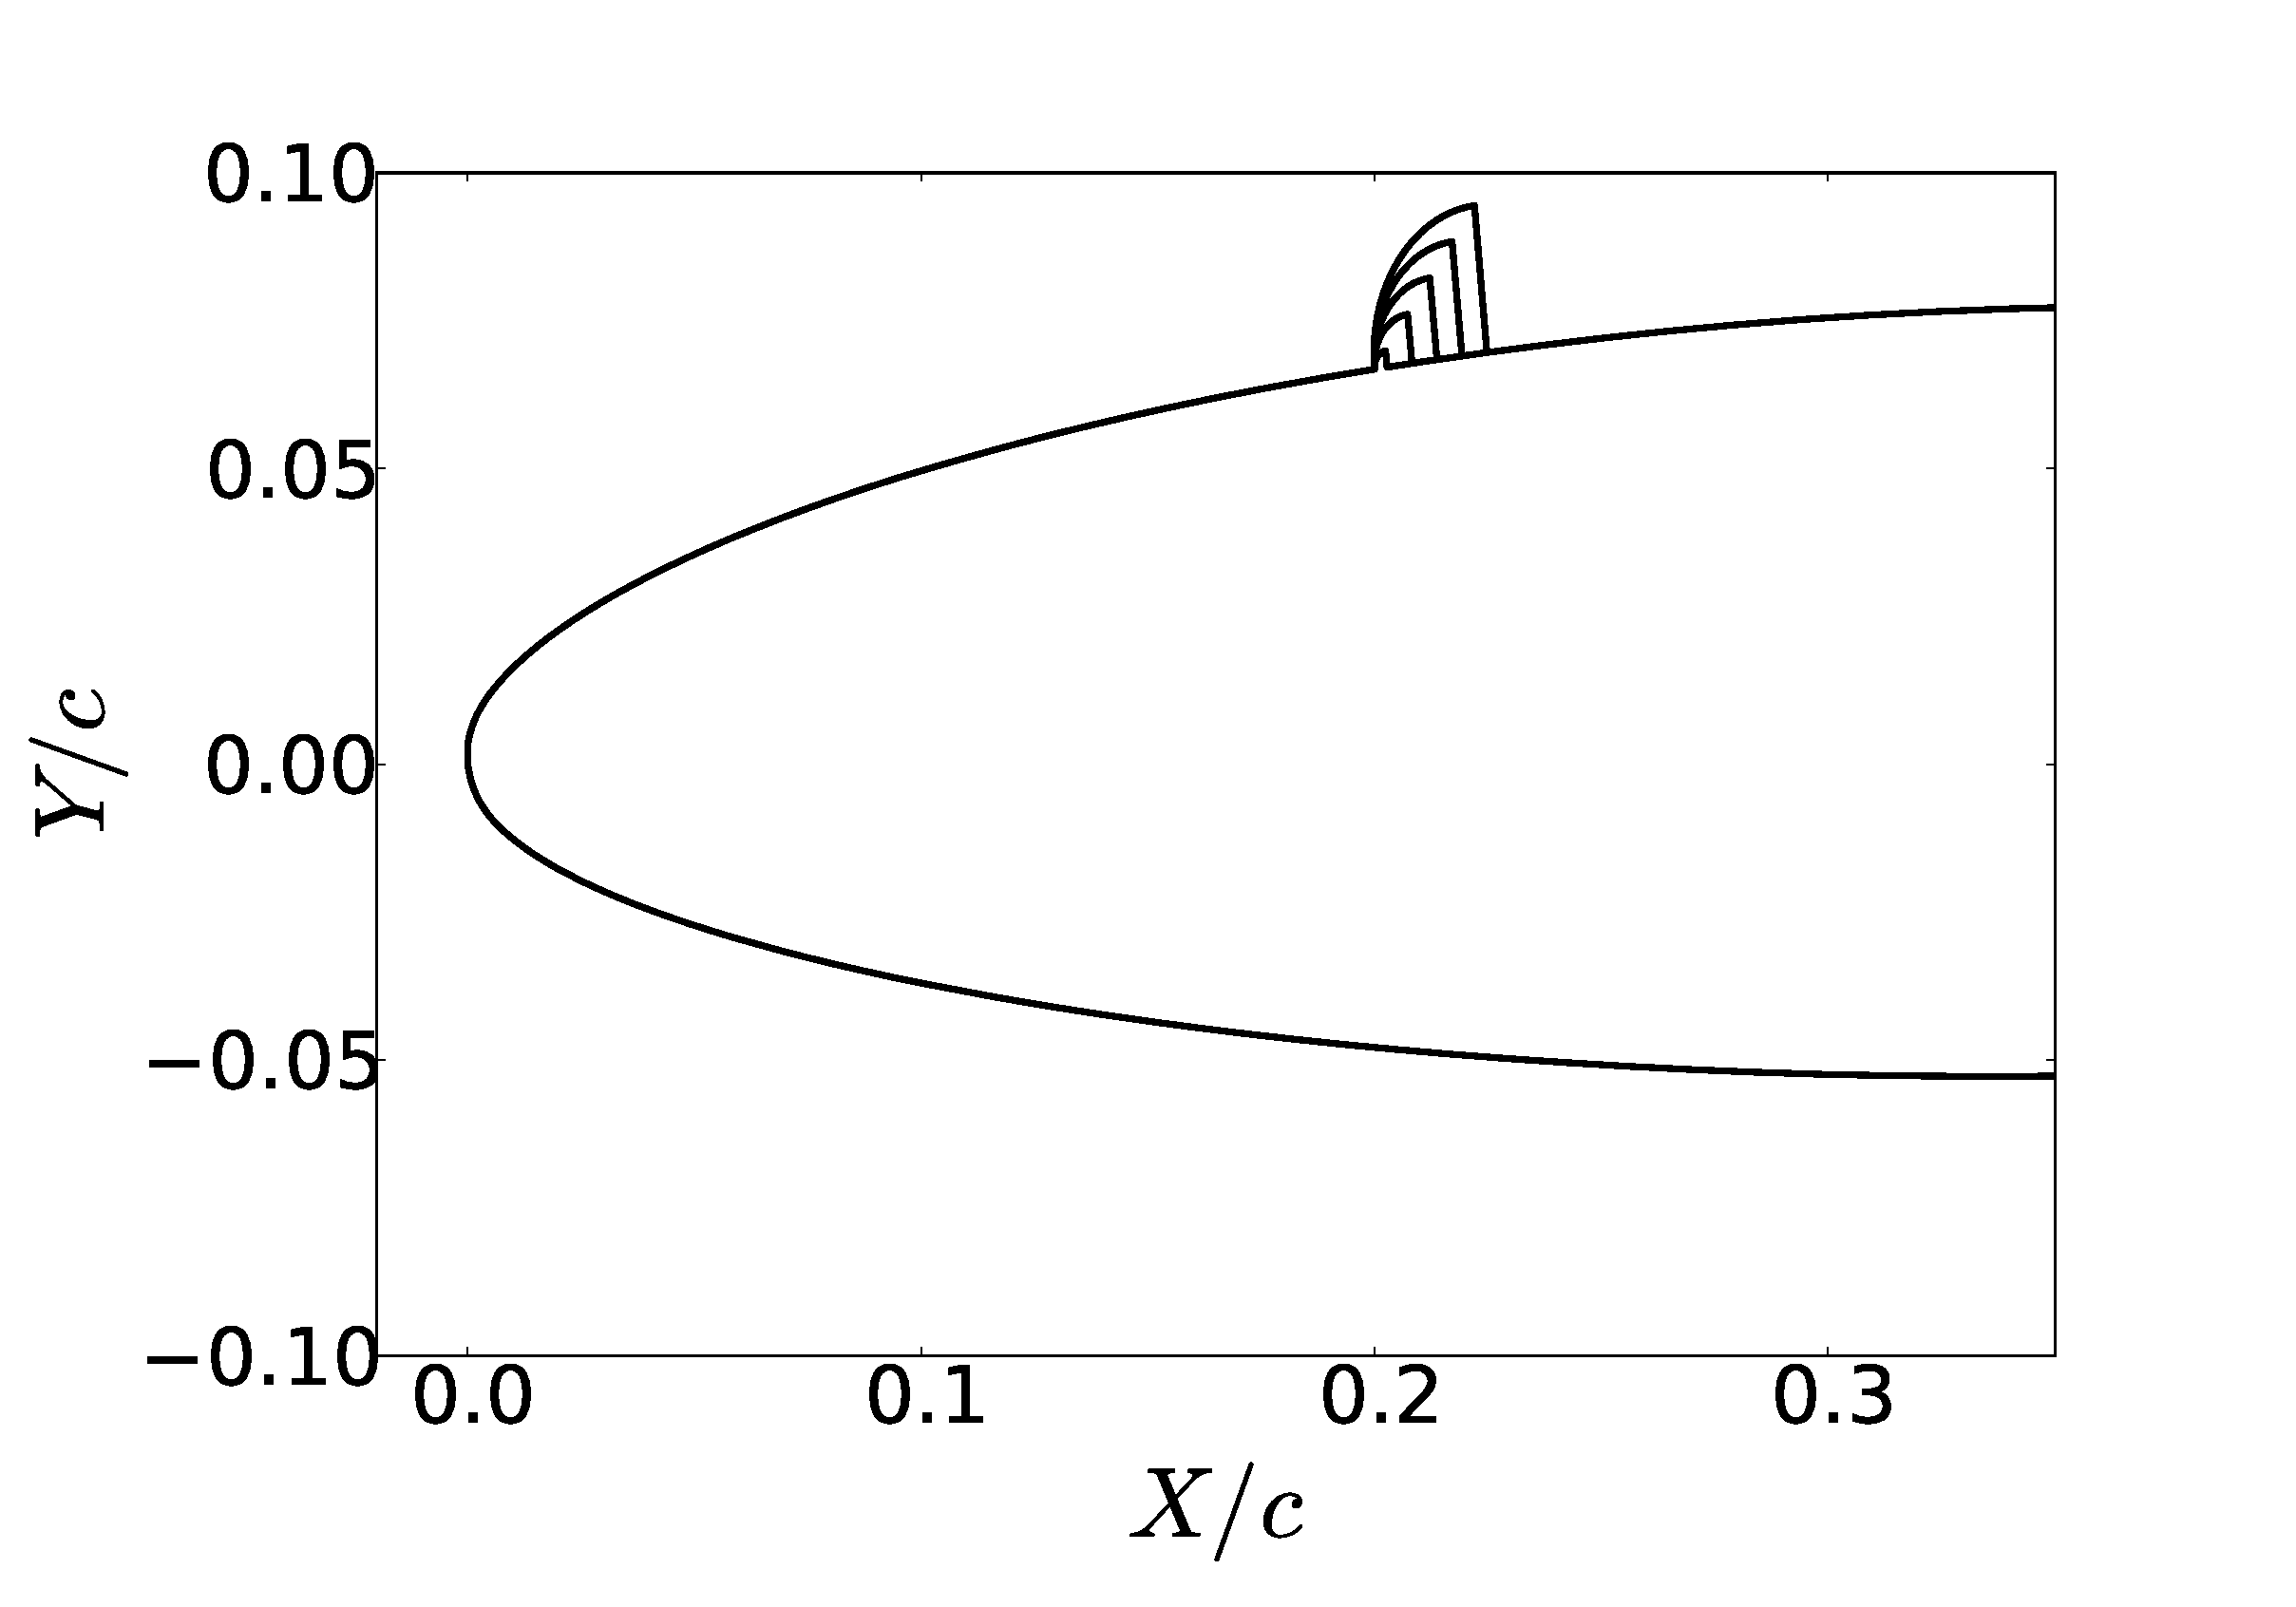
\includegraphics[width=0.95\textwidth]{RidgeRVariation} \\
    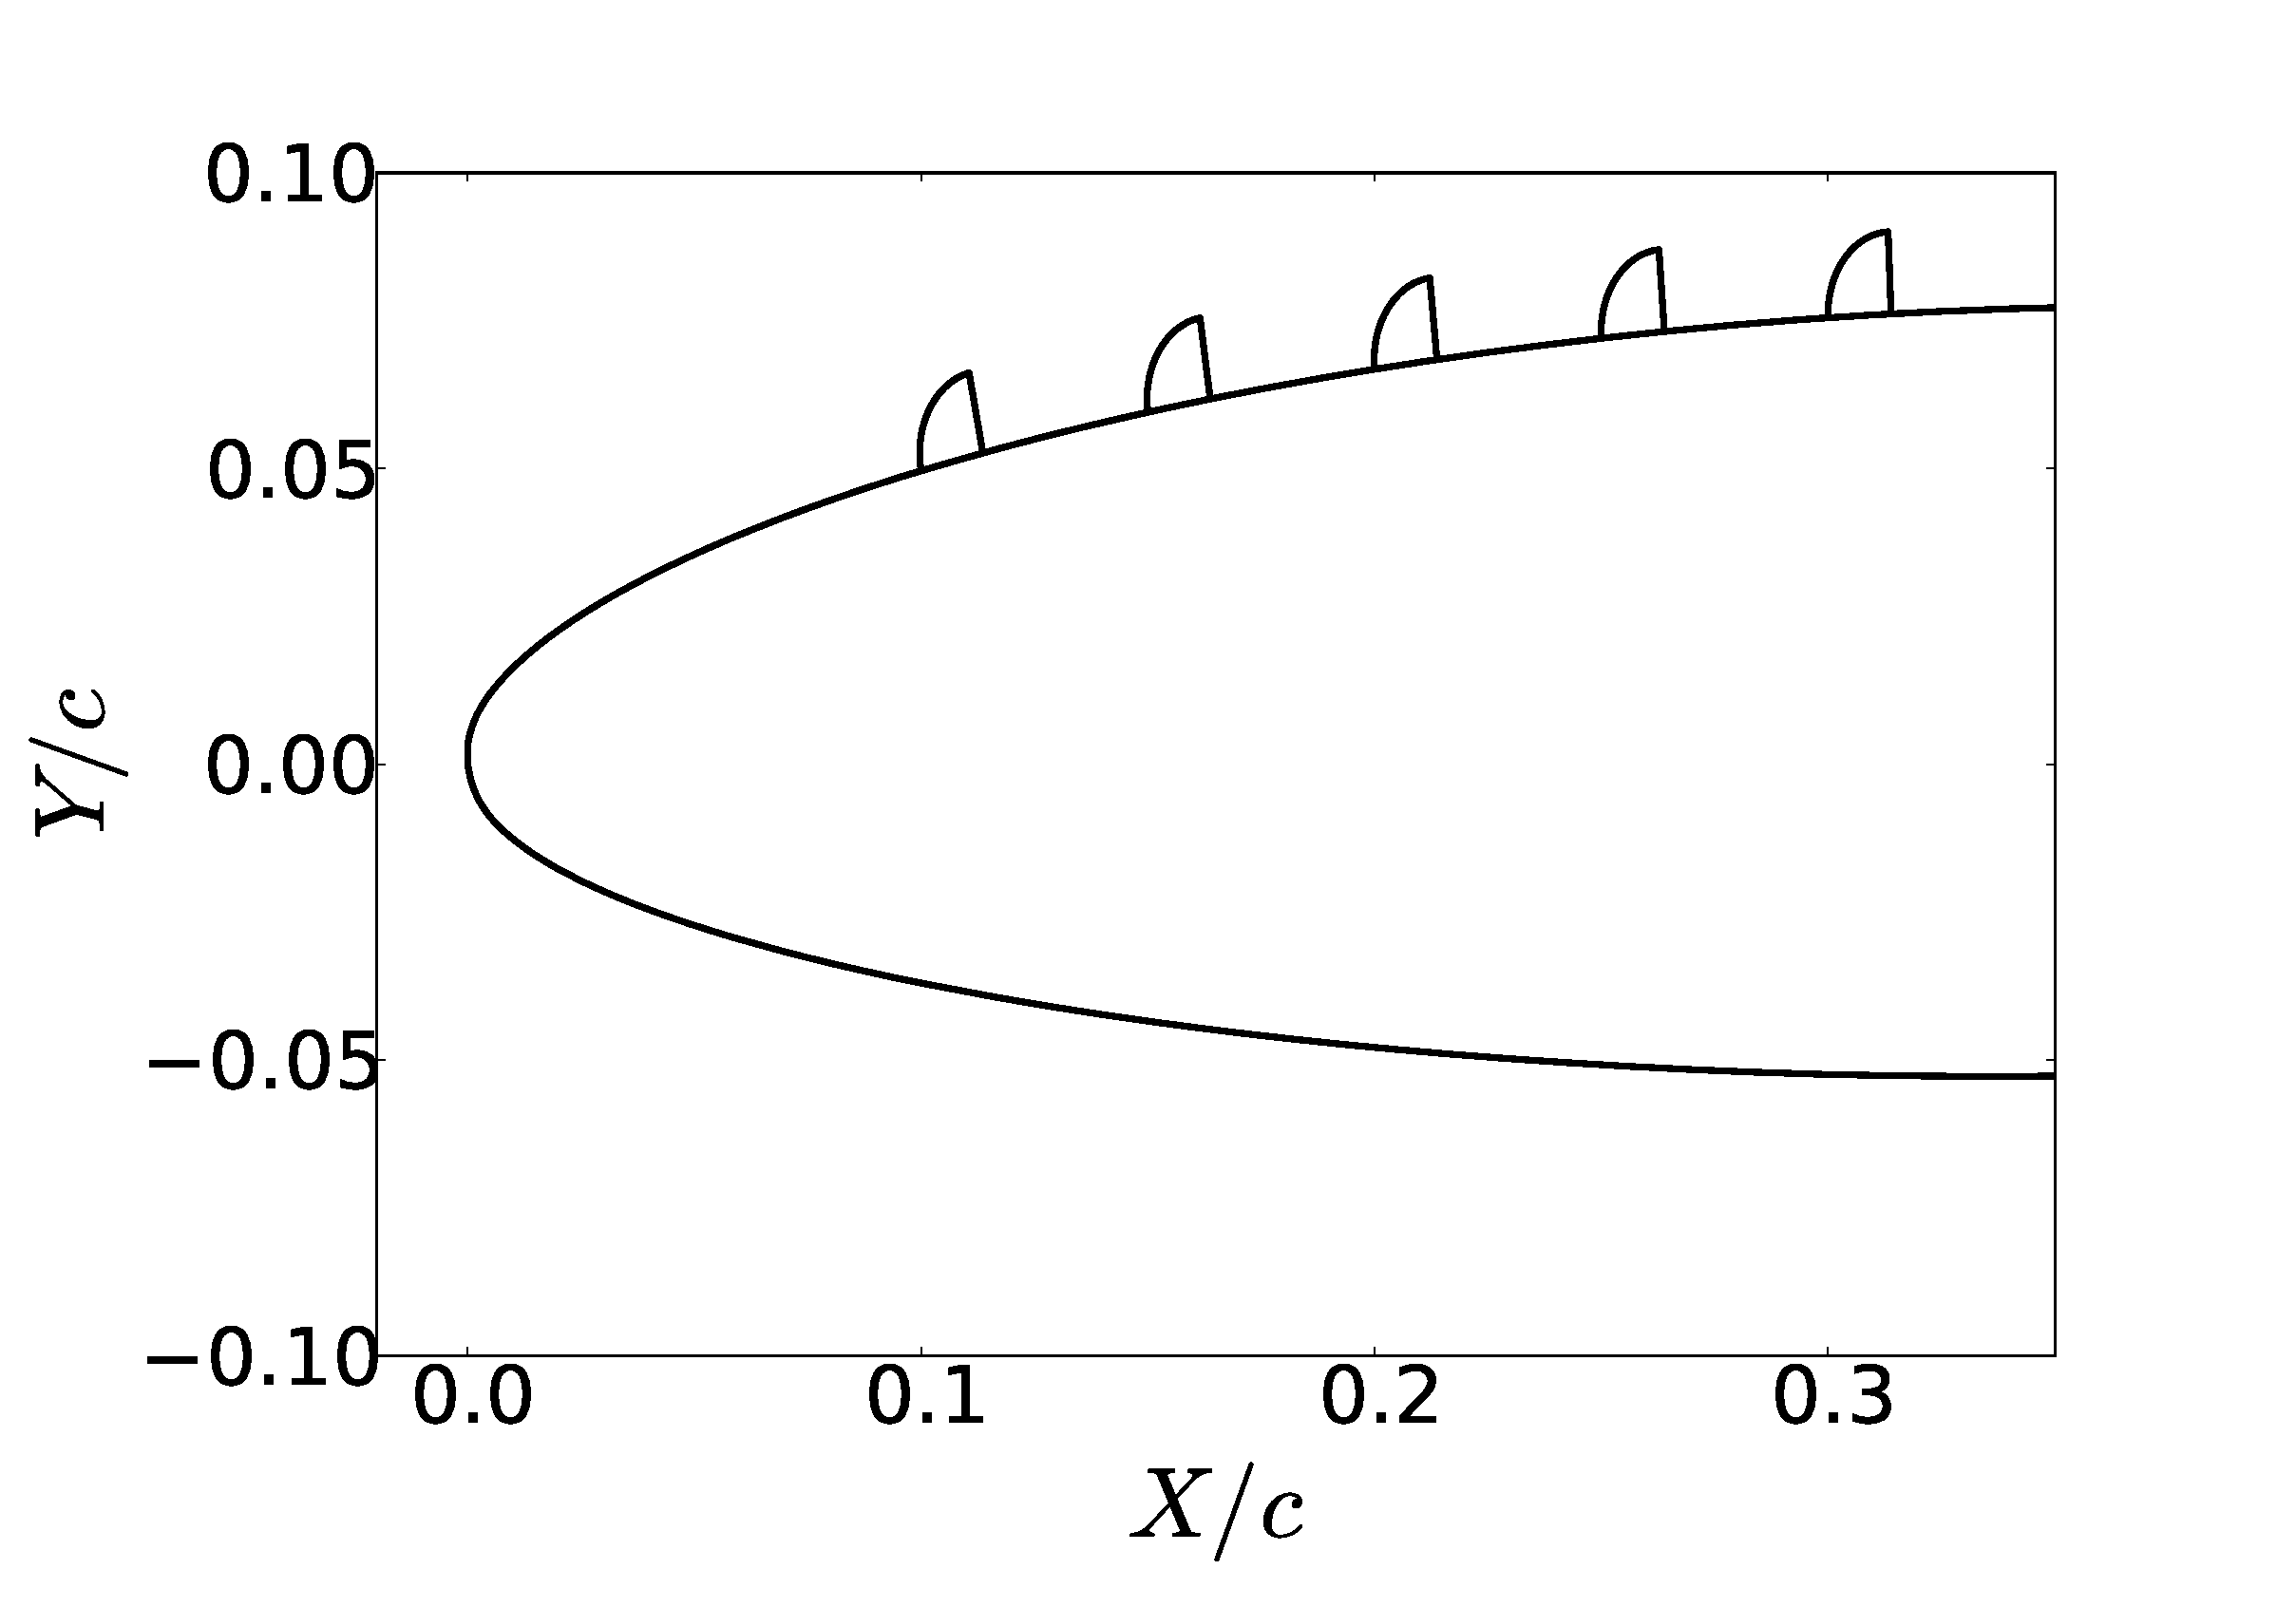
\includegraphics[width=0.95\textwidth]{RidgeSVariation} \\
    {\bf Ridge}
  \column{0.33\textwidth}
    \centering
    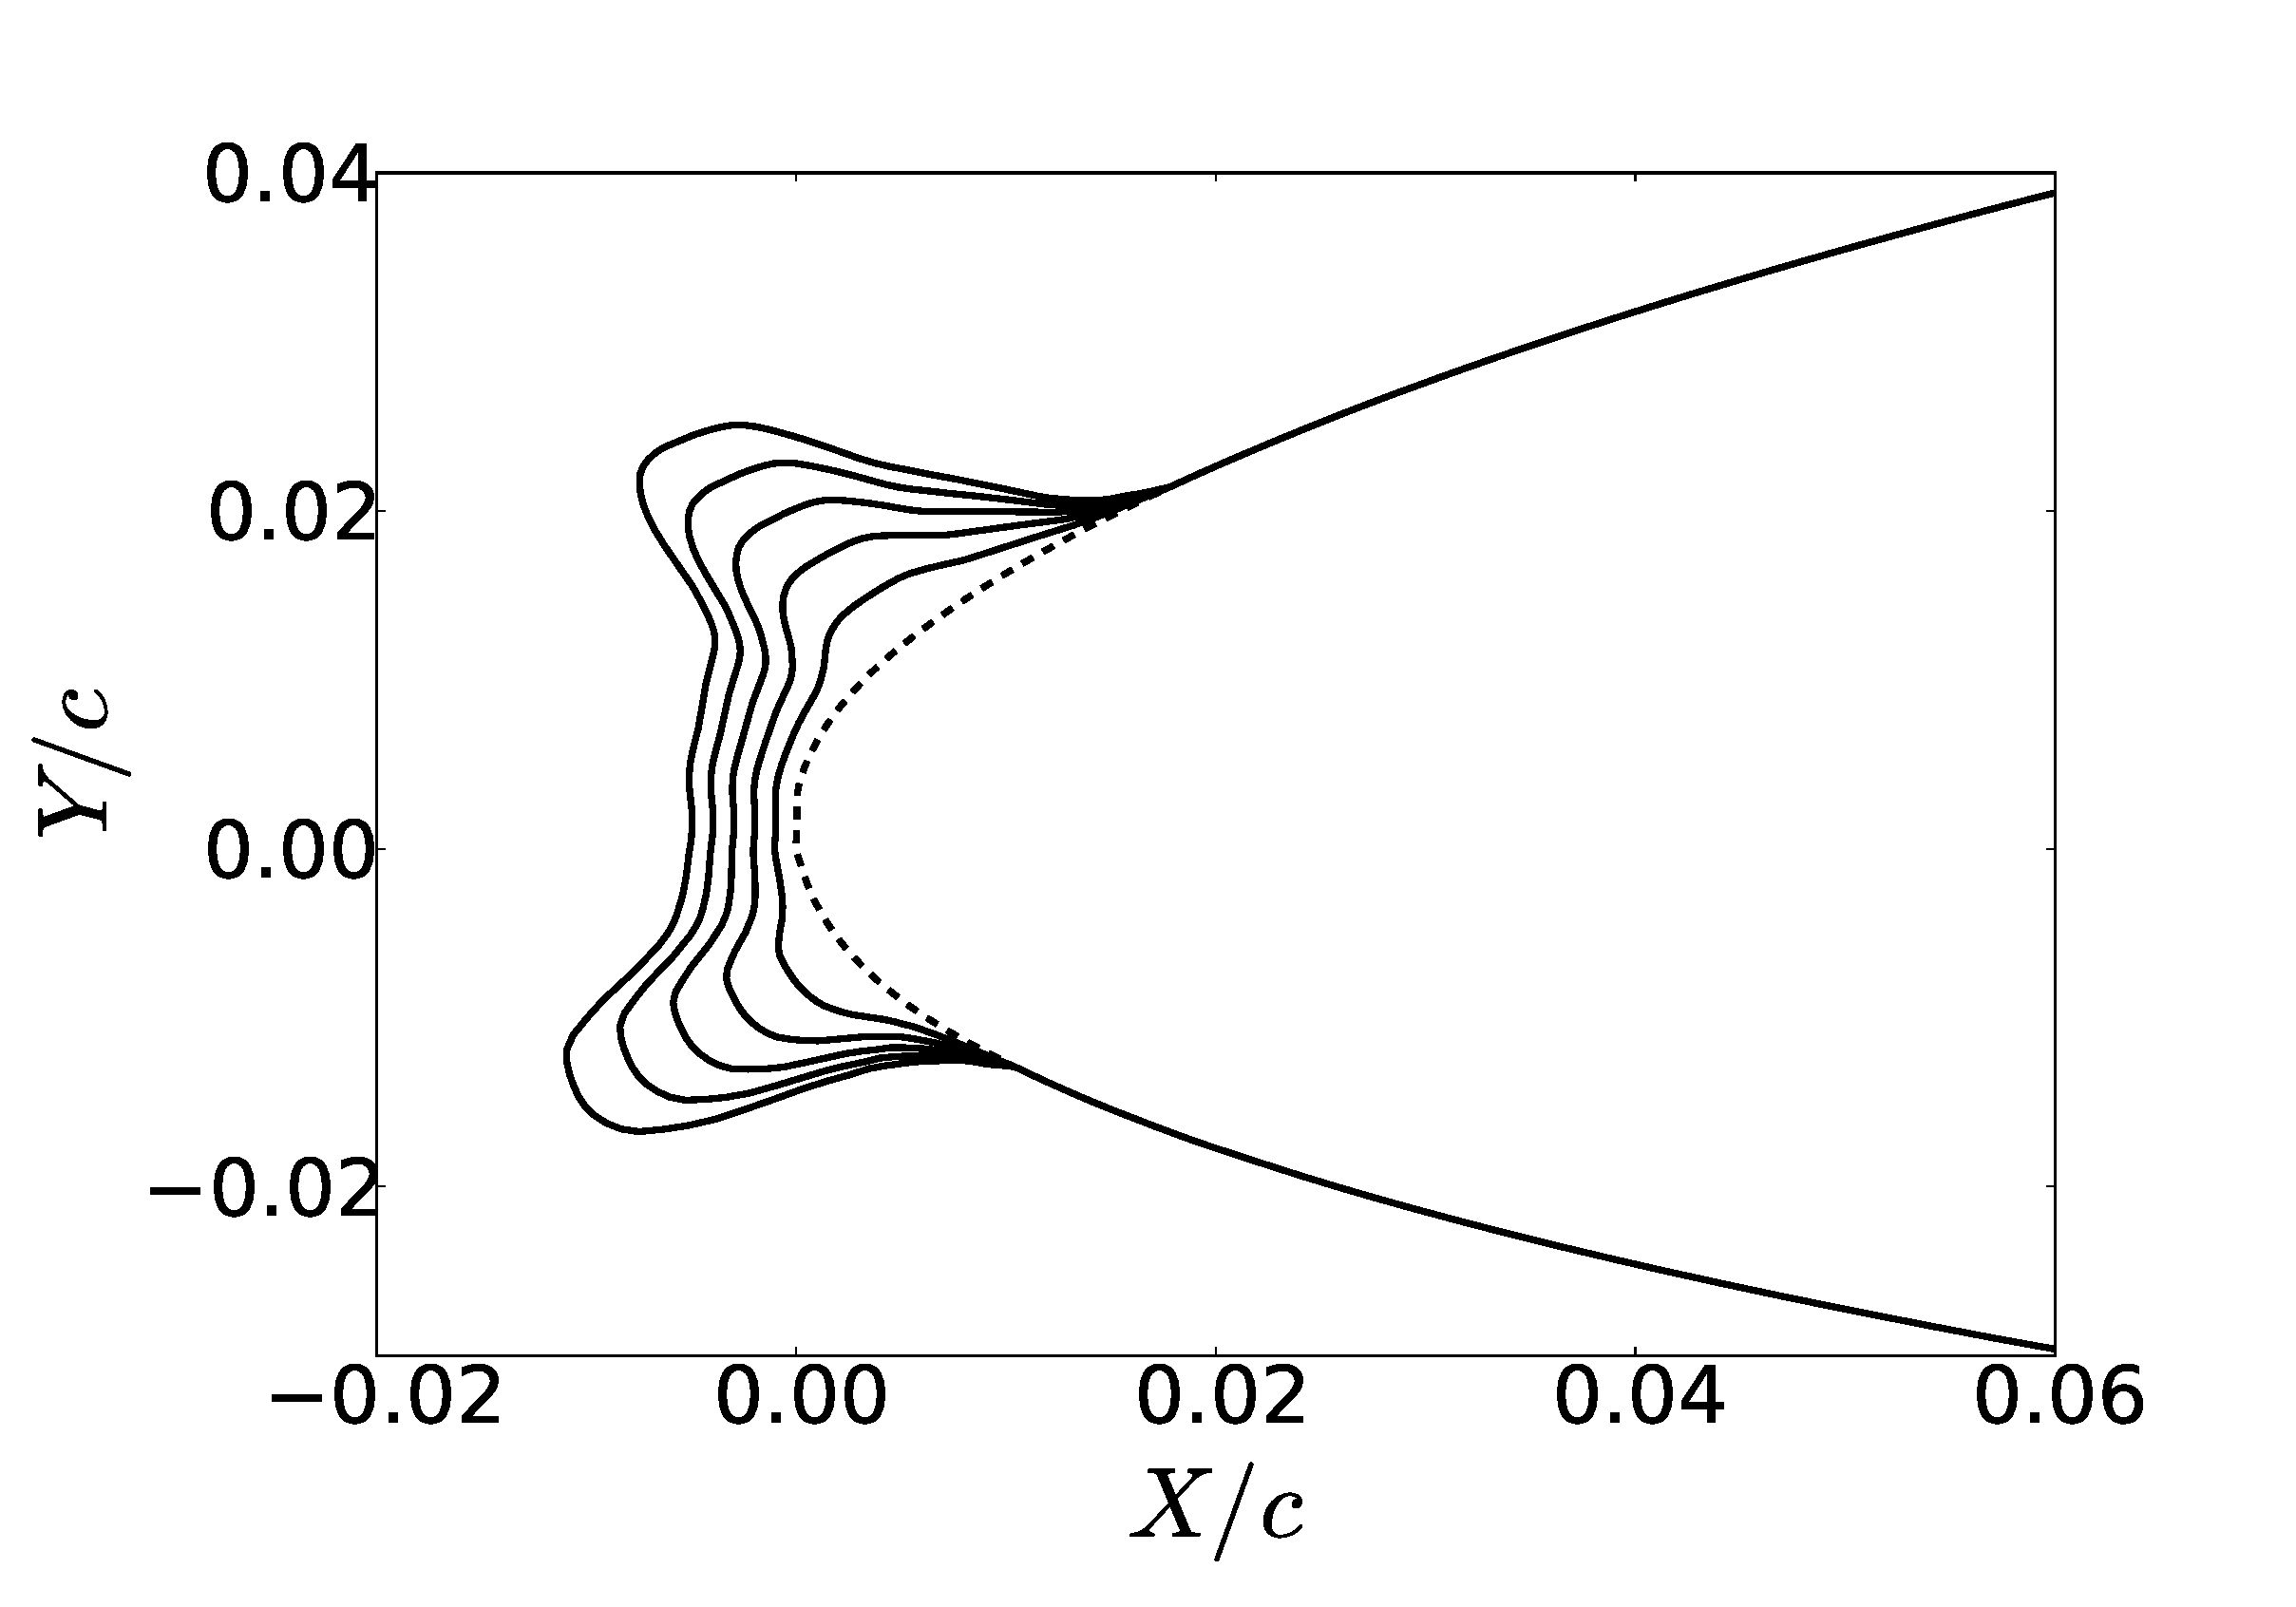
\includegraphics[width=0.95\textwidth]{HornHVariation} \\
    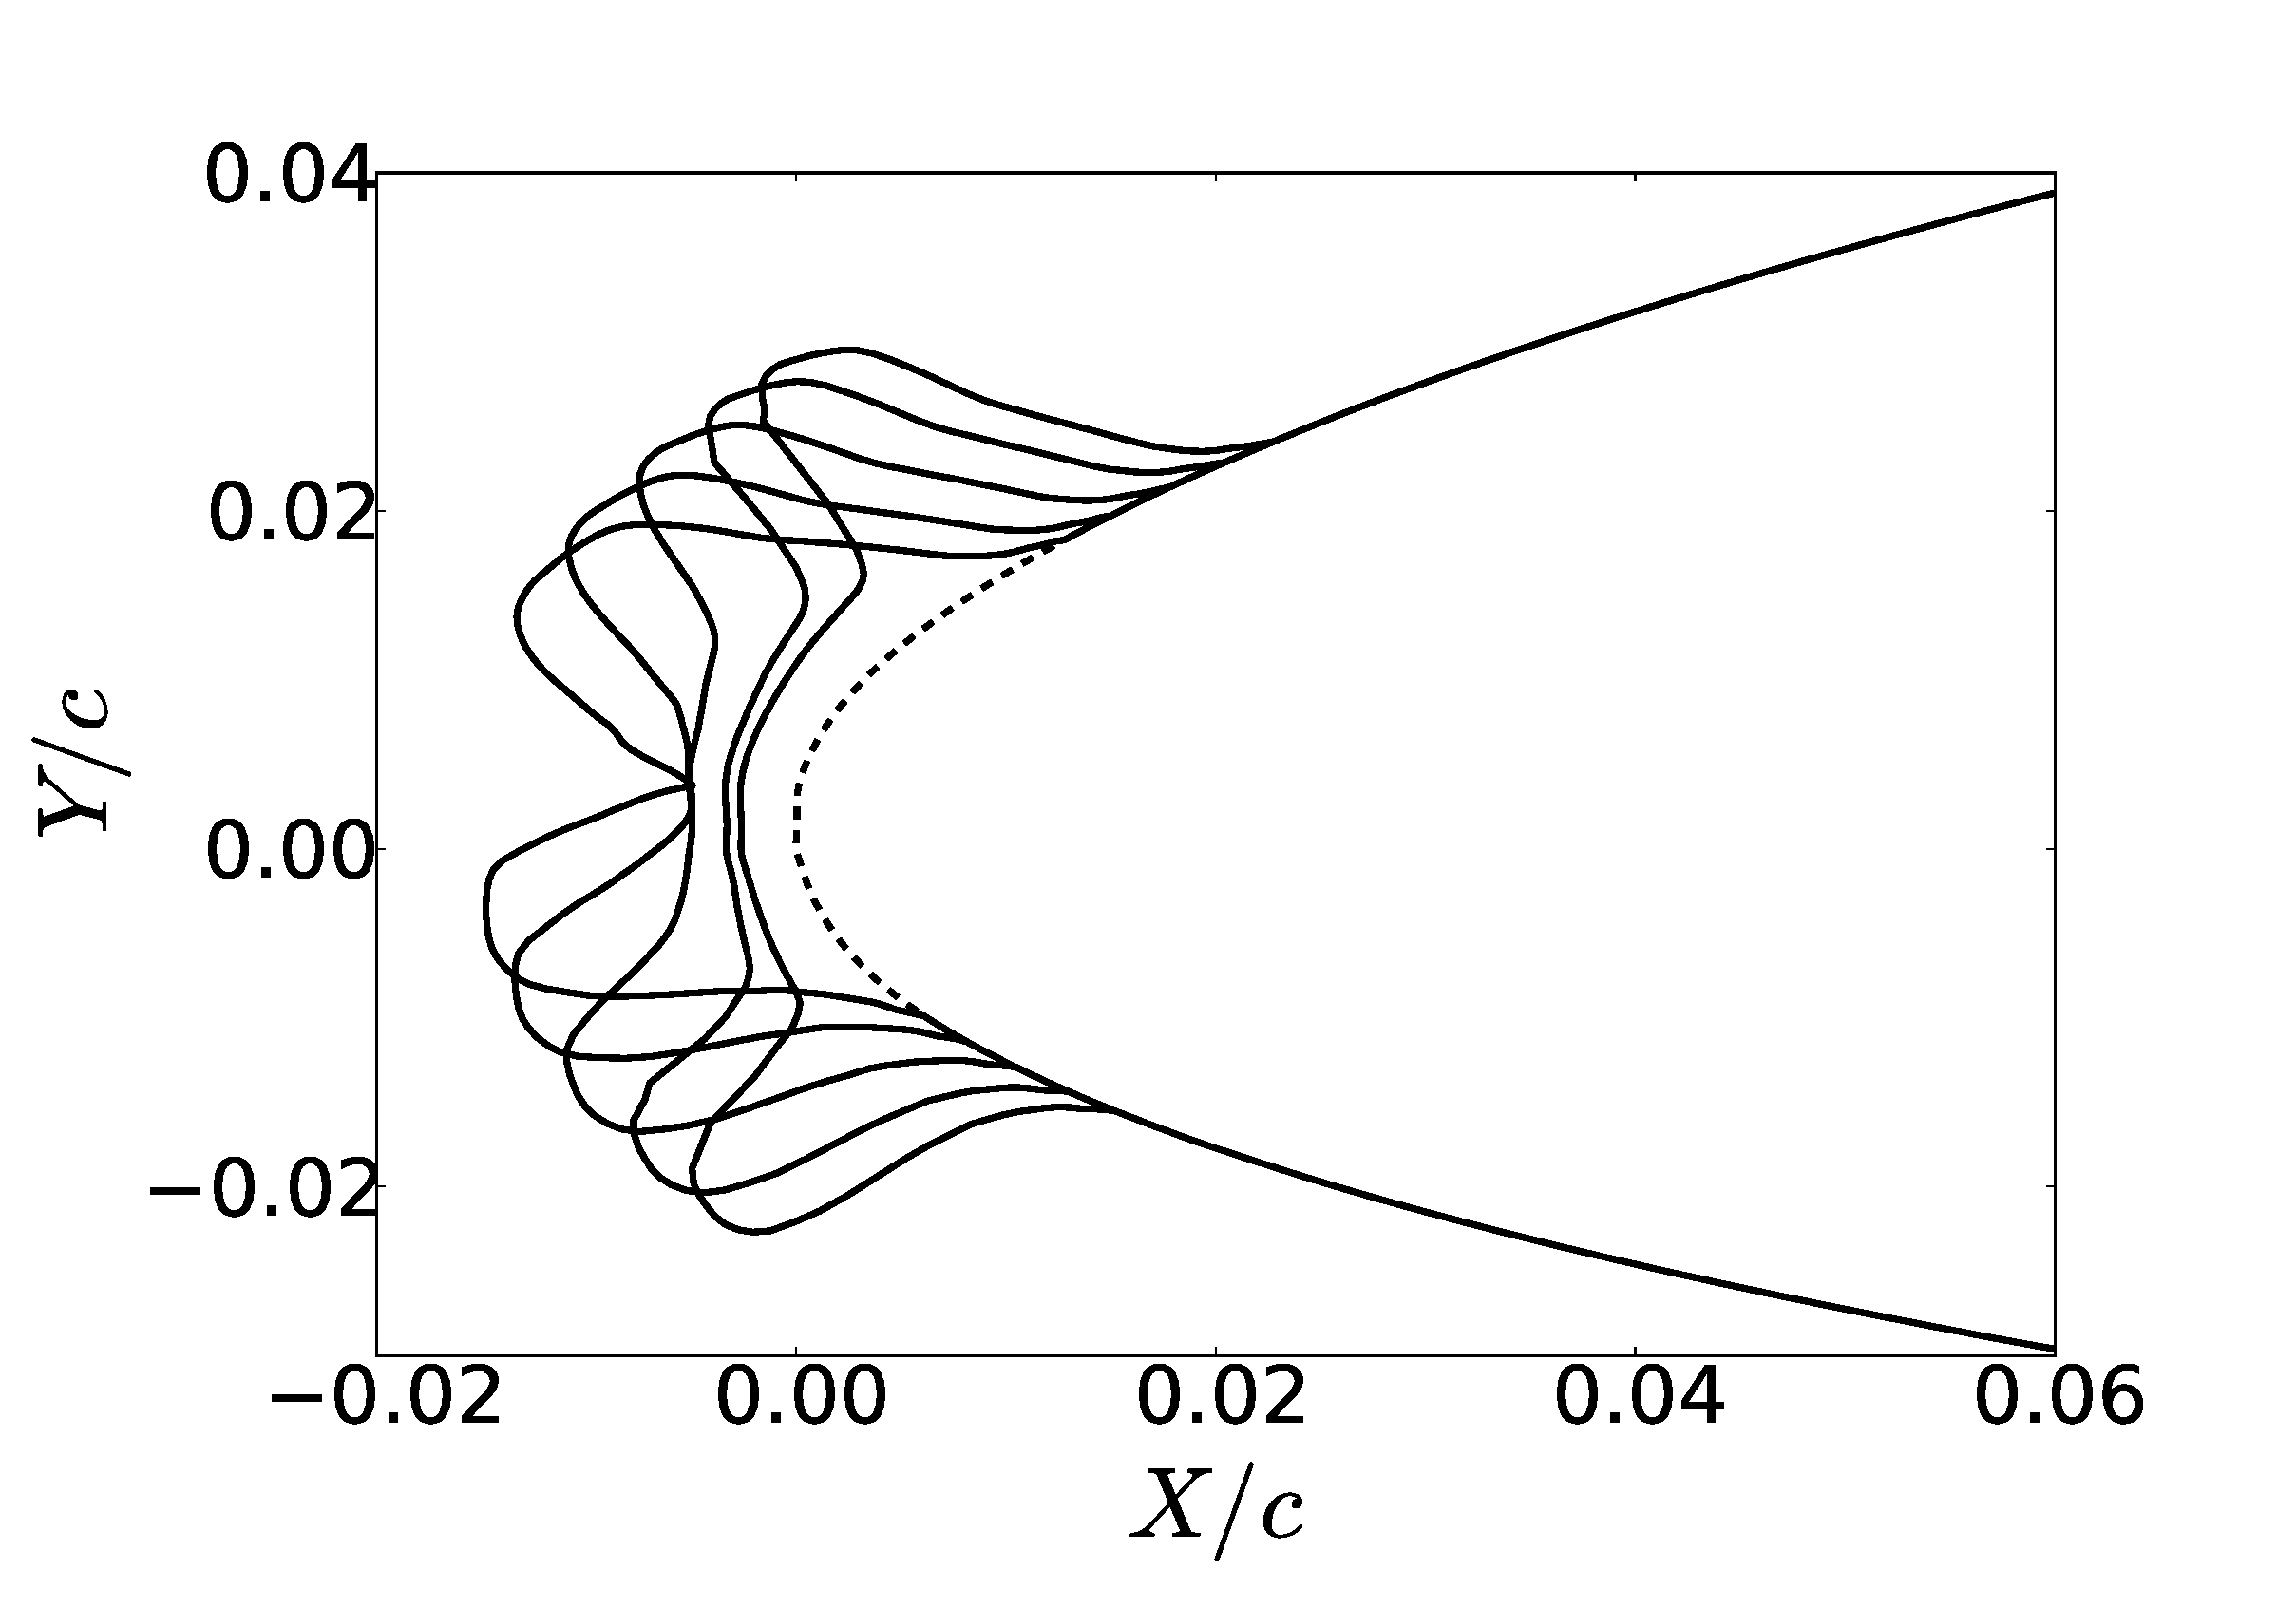
\includegraphics[width=0.95\textwidth]{HornSVariation} \\
    {\bf Horn}
  \column{0.33\textwidth}
    \centering    
    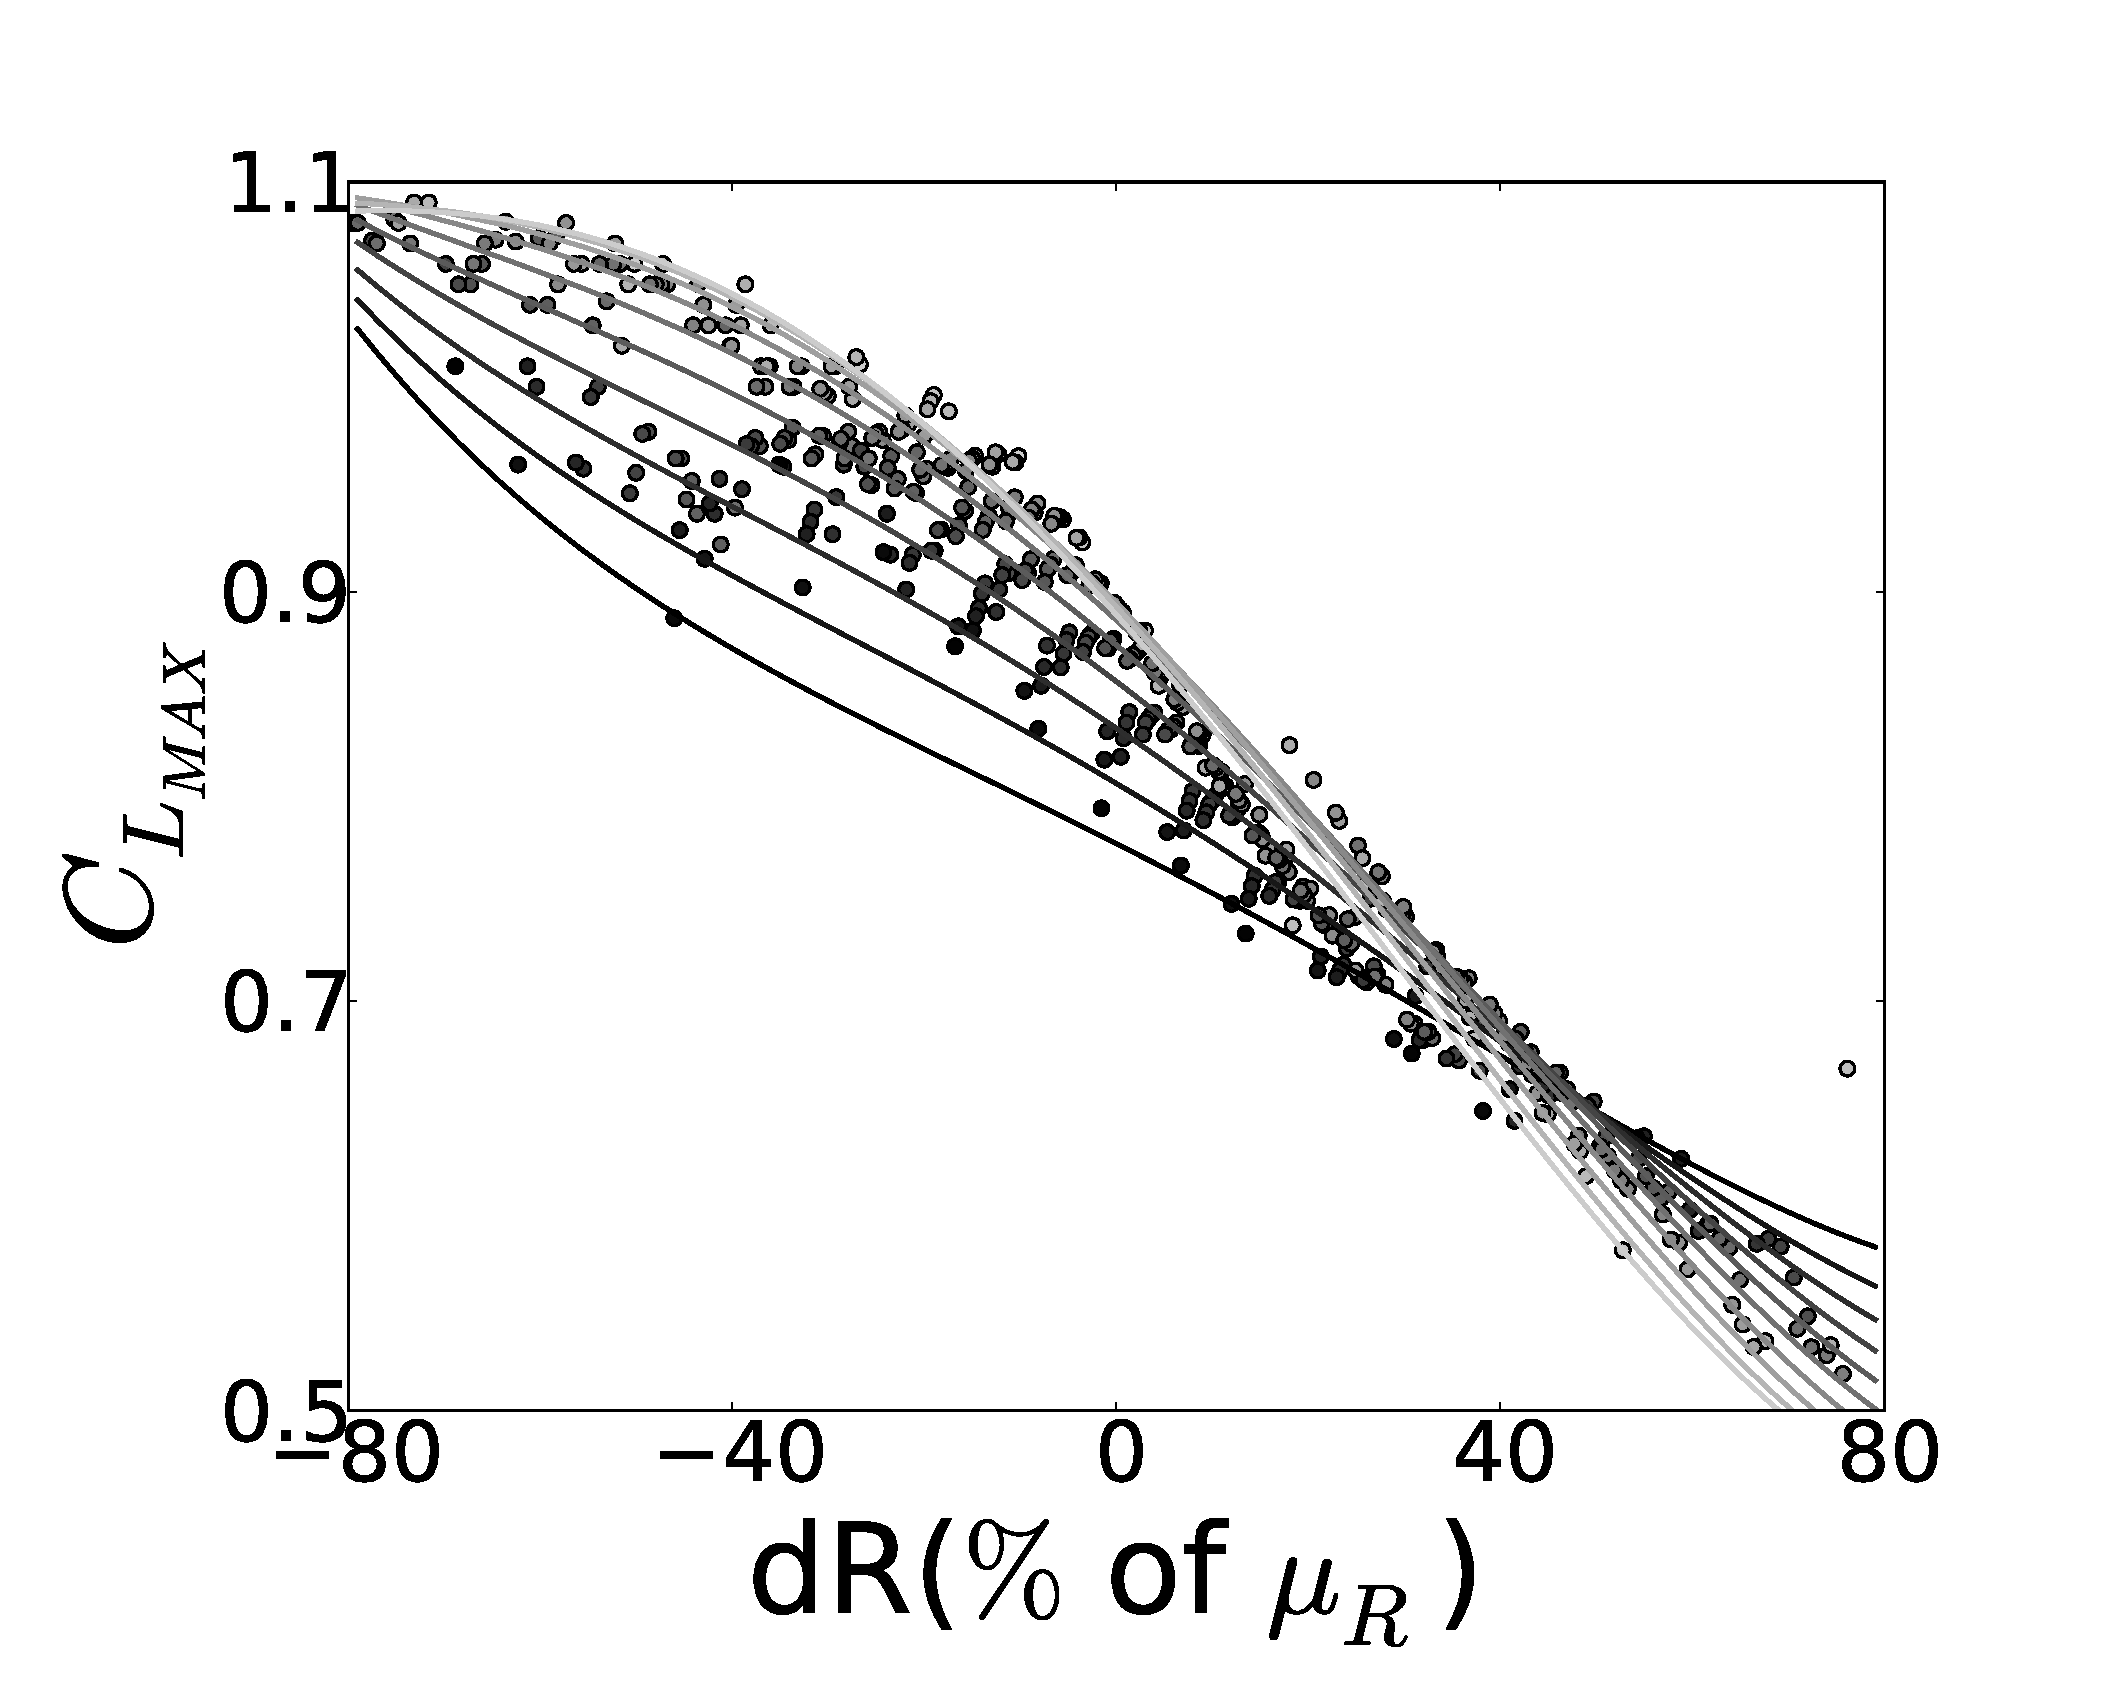
\includegraphics[width=0.9\textwidth]{MC_surrogate_LargeUnc_CL} \\
    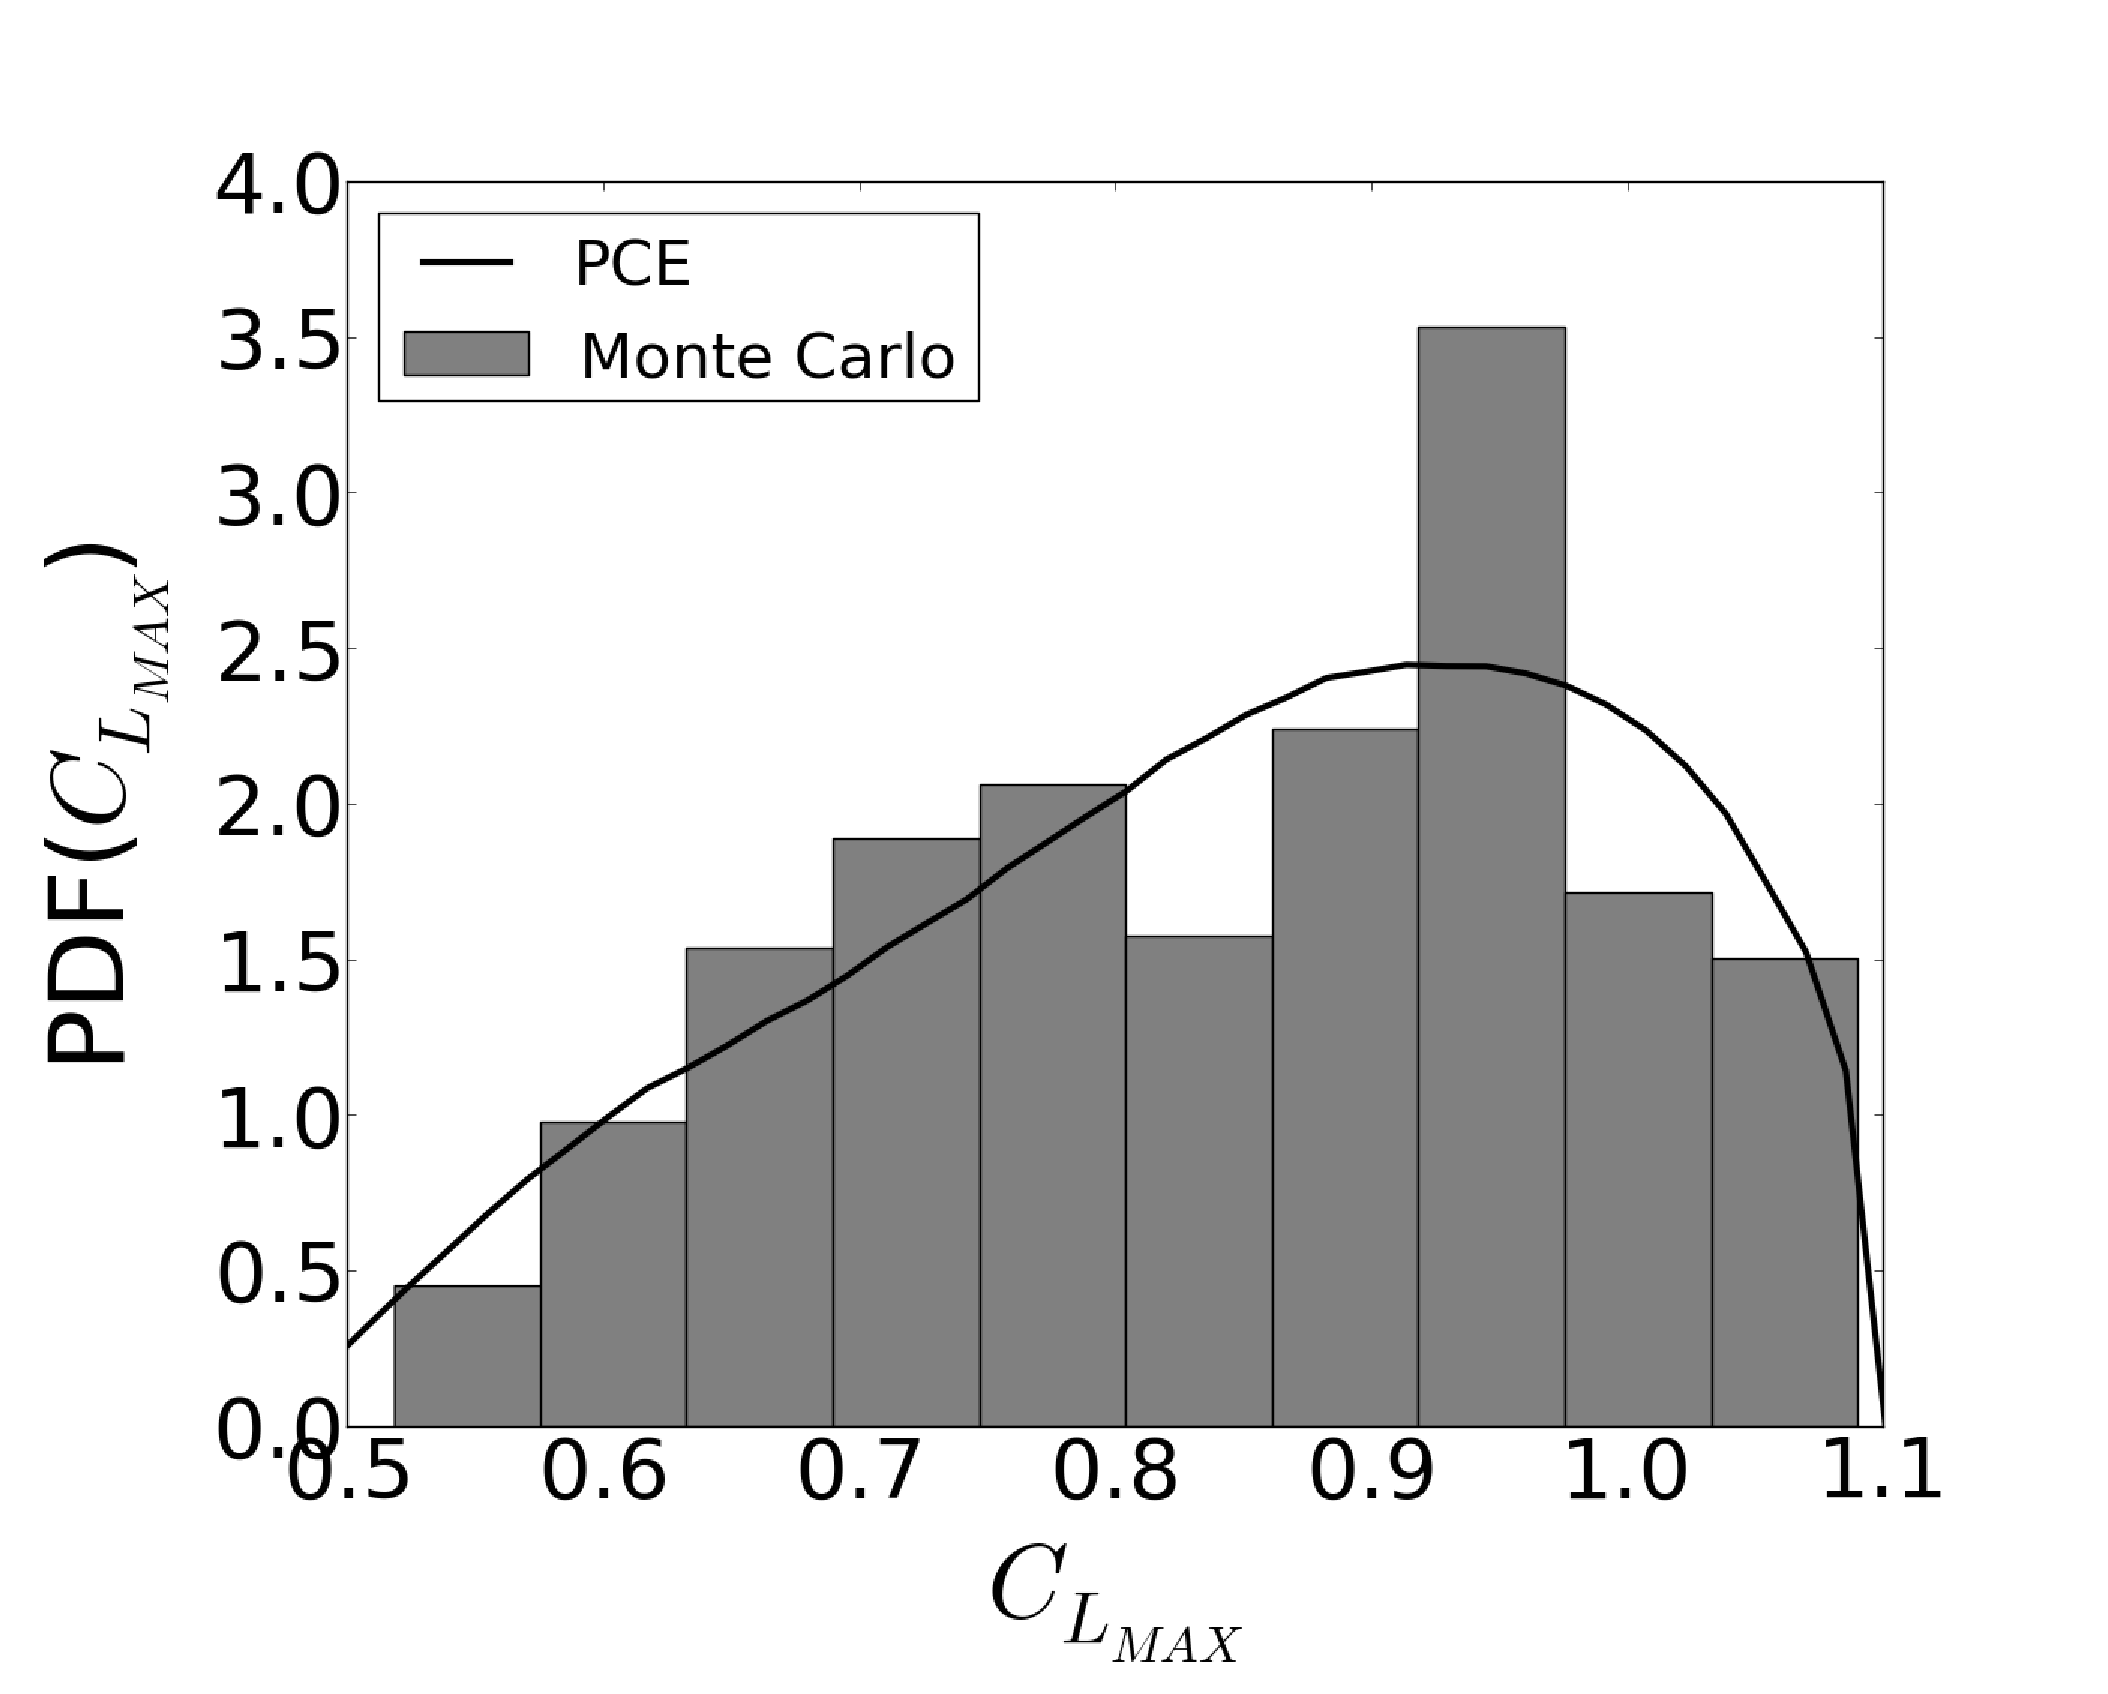
\includegraphics[width=0.9\textwidth]{MCgpcPDFLargeUnc_CL} \\
    {\bf Statistics}
\end{columns}

\begin{itemize}
\item Previous study examined parameterized ridge and horn ice
  shapes\footnote{DeGennaro A., Rowley C.W., and Martinelli,
L. \emph{Uncertainty Quantification for Airfoil Icing using Polynomial Chaos Expansions}. To appear in Journal of Aircraft, 2015.
 }
\item Approach was heuristic, not directly based on observed shape
  variations
\item Parameter space was low dimensional; no low-dimensional modeling
\end{itemize}
\end{frame}
\section{Methodology}
\label{sec-2}
\begin{frame}
\frametitle{Low-Dimensional Modeling}
\label{sec-2-1}


\begin{itemize}
\item The space of all ice shapes is infinite dimensional
\item Consider small number of parameters that describe \emph{likely} shapes
\item Analyze database of shapes from experiments/simulations
\item \textbf{Proper Orthogonal Decomposition} \footnote{Holmes P. et. al. \emph{Turbulence, Coherent Structures, Dynamical Systems and Symmetry}, Cambridge University Press, New York, 2012.
 }
\begin{itemize}
\item Assume database of \emph{M} ice shapes
\item Each individual ice shape can be represented by a vector $\bv{x}
    \in \mathbb{R}^N$
\item Approximate $\bv{x}$ using some basis vectors $\psi_i$:
    \begin{equation*}
      \bv{x} \approx \sum_{i=1}^P a_i \psi_i
    \end{equation*}
\item Choose basis vectors to be the eigenvectors of the dataset
    covariance matrix
    \begin{equation*}
    \begin{aligned}
      \mathcal{R} \psi_k = \lambda_k \psi_k& \text{   where:   } \\ 
      \mathcal{R} = \frac{1}{M}\mathbf{X}\mathbf{X}^T \text{   and:   }&
      \mathbf{X} =
       \begin{bmatrix}
        \vline & & \vline \\
        x_1 & \cdots & x_M \\
        \vline & & \vline \\
       \end{bmatrix}
    \end{aligned}
    \end{equation*}
\end{itemize}
\end{itemize}
\end{frame}
\begin{frame}
\frametitle{Polynomial Chaos Expansions (PCE)}
\label{sec-2-2}


\begin{itemize}
\item \textbf{Polynomial Chaos Framework} \footnote{Xiu D. \emph{Numerical Methods for Stochastic Computations: A Spectral Method Approach}. Princeton University Press, 2010.
 }
\begin{itemize}
\item Let $\bv{Z} = (Z_1 \ldots Z_d)$ be $d$ random variables with PDF
    $\rho(\bv{Z})$ that parameterize ice
\item Let $\lbrace \Phi_k \rbrace$ denote the set of polynomials
    which are orthogonal w.r.t. $\rho(\bv{Z})$
\item Let $y(\bv{Z})$ denote the mapping from $\bv{Z}$ to an aerodynamic
    performance metric
\end{itemize}
\item \textbf{Probabilistic Collocation Method:}
\begin{itemize}
\item \emph{Representation} 
    \begin{equation*}
      y(\bv{Z}) \approx \sum_{|i|=0}^N y_i \Phi_i(\bv{Z})
    \end{equation*}
\item \emph{Orthonormality} 
    \begin{equation*}
    \begin{aligned}
      \ip{f}{g} &= \int_{\Gamma} f(\bv{z})g(\bv{z}) \rho(\bv{z}) d\bv{z} \\
      \ip{\Phi_i}{\Phi_j} &= \delta_{ij}
    \end{aligned}
    \end{equation*}
\item \emph{Quadrature} 
    \begin{equation*}
      y_k = \ip{y}{\Phi_k} \approx \sum_{i=0}^{Q}
    y(\bv{Z}^{(k)}) \Phi_k(\bv{Z}^{(k)}) w_k
    \end{equation*}
\end{itemize}
\end{itemize}
\end{frame}
\begin{frame}
\frametitle{PCE with Sparse Grids}
\label{sec-2-3}


\begin{columns}[c]
  \column{0.7\textwidth}
    \centering
    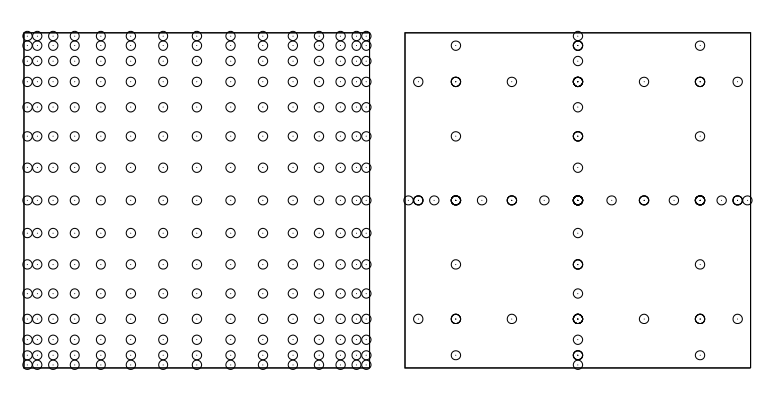
\includegraphics[width=0.95\textwidth]{SparseGrid1} \\
    \bf{Full Tensor Product vs. Sparse Grid}
  \column{0.3\textwidth}
    \centering
    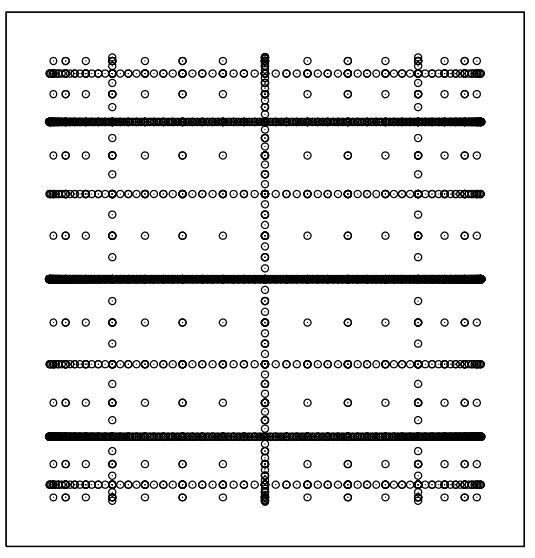
\includegraphics[width=0.95\textwidth]{SparseGrid2} \\
    {\bf Anisotropic Grid}
\end{columns}

\begin{itemize}
\item \textbf{Sparse Grids}\footnote{LeMaitre O. \emph{Spectral Methods for Uncertainty Quantification}. Springer, 2010.
 }
\begin{itemize}
\item \emph{Efficient}: Only a subset of the full quadrature grid is used
\begin{itemize}
\item For $d >> 1$, number of samples scales as $2^N {N+d \choose d} <<
      (N+1)^d$
\end{itemize}
\item \emph{Adaptive}: Start with a coarse mesh, adaptively refine until
    achieve desired resolution
\item \emph{Anisotropic}: Refine grid in most ``important'' directions
\item Implemented in DAKOTA\footnote{Adams et. al. \emph{DAKOTA, A Multilevel Parallel Object-Oriented Framework for Design Optimization\ldots{}} V. 5.3 User's
Manual. SAND2010-2183.
 } (open-source UQ code)
\end{itemize}
\end{itemize}
\end{frame}
\section{Simulation Dataset}
\label{sec-3}
\begin{frame}
\frametitle{Dataset Description}
\label{sec-3-1}

\begin{figure}
  \centering
  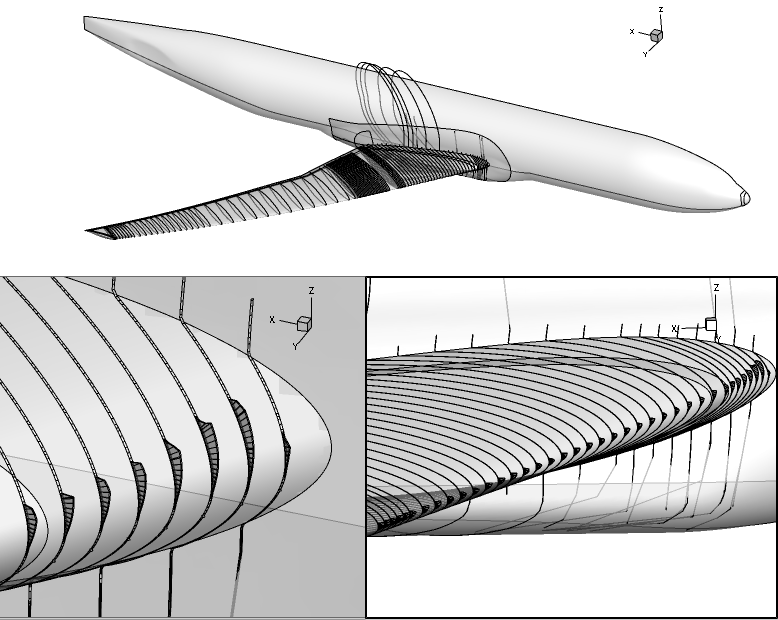
\includegraphics[width=0.6\textwidth]{CRMHorn}
\end{figure}

\begin{itemize}
\item NASA Common Research Model (CRM), $65\%$ scale\footnote{Broeren A. et. al. \emph{Swept-Wing Ice Accretion Characterization and Aerodynamics}, AIAA 2013-2824.
 }
\begin{itemize}
\item 45 min accretion time, altitude = 10,000 ft, velocity = 232 knots,
    temperature = $-4^{\text{o}}$ C, MVD = 20 $\mu m$, LWC = 0.55
    $g/m^3$
\end{itemize}
\end{itemize}
\end{frame}
\begin{frame}
\frametitle{Low-Dimensional Modeling of Dataset}
\label{sec-3-2}

\begin{columns}[c]
  \column{0.3\textwidth}
    \centering
    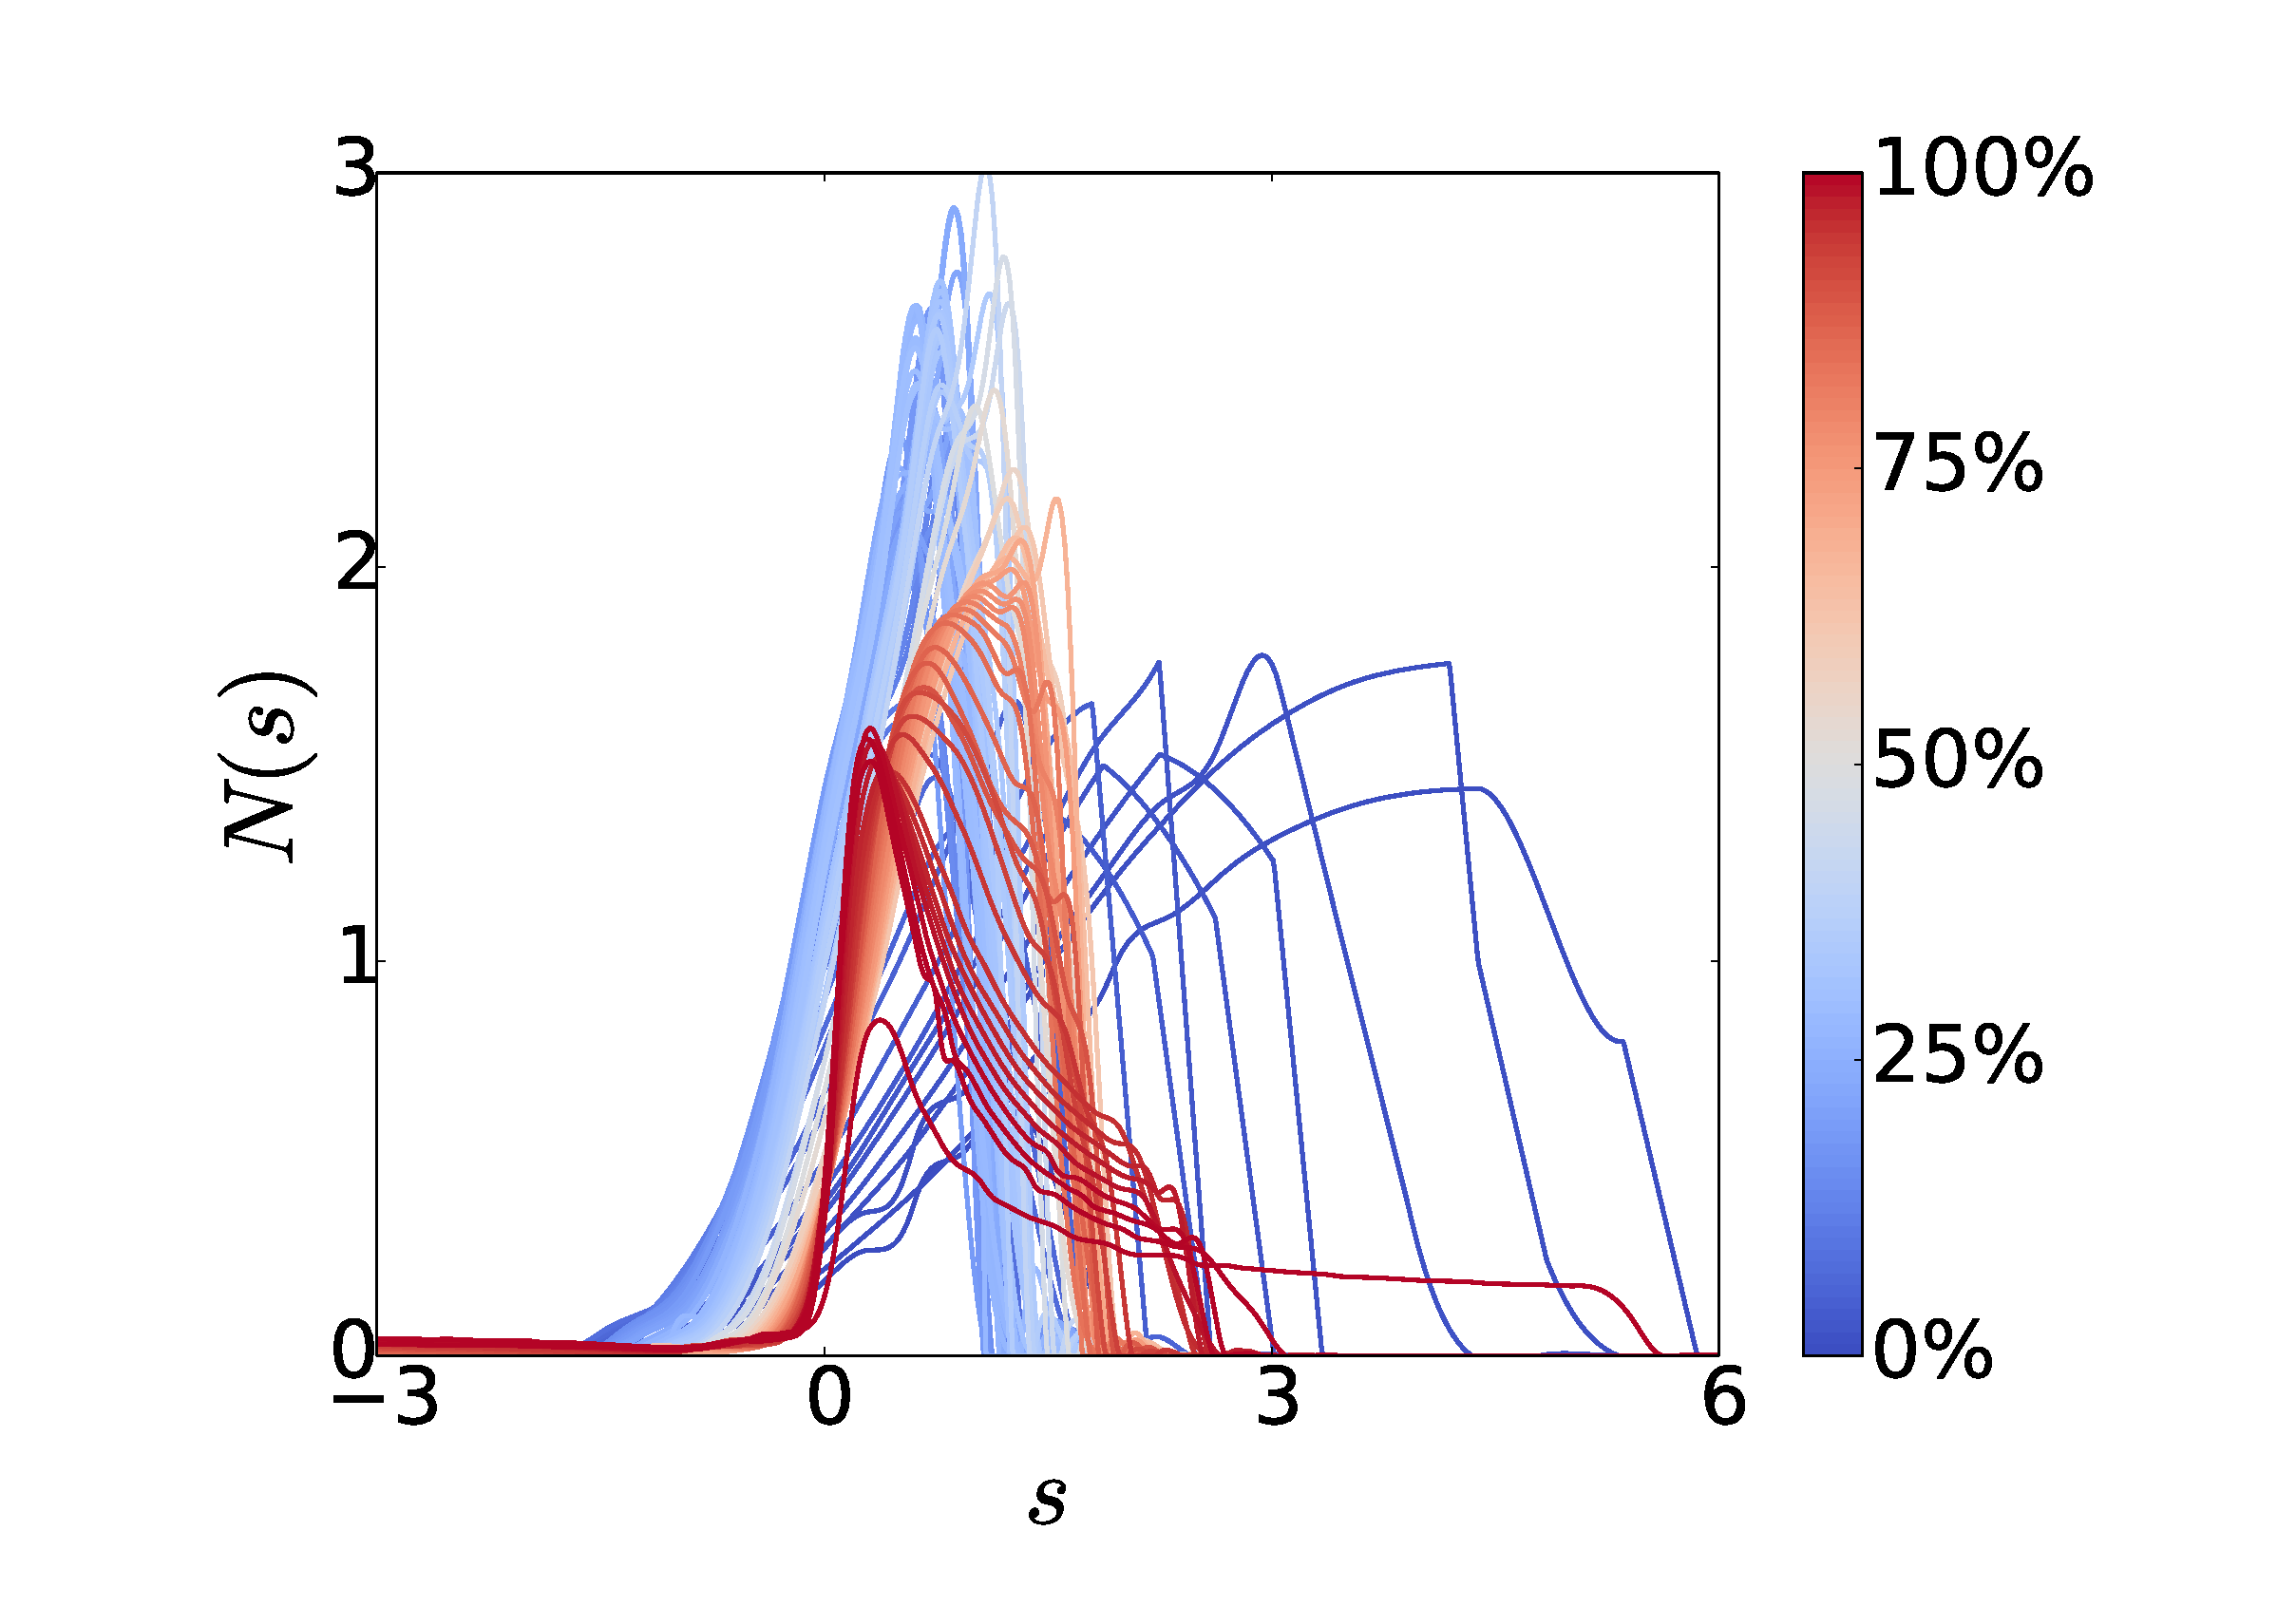
\includegraphics[width=1.3\textwidth]{HornsUnaligned} \\
    \bf{Original Data}
  \column{0.3\textwidth}
    \centering
    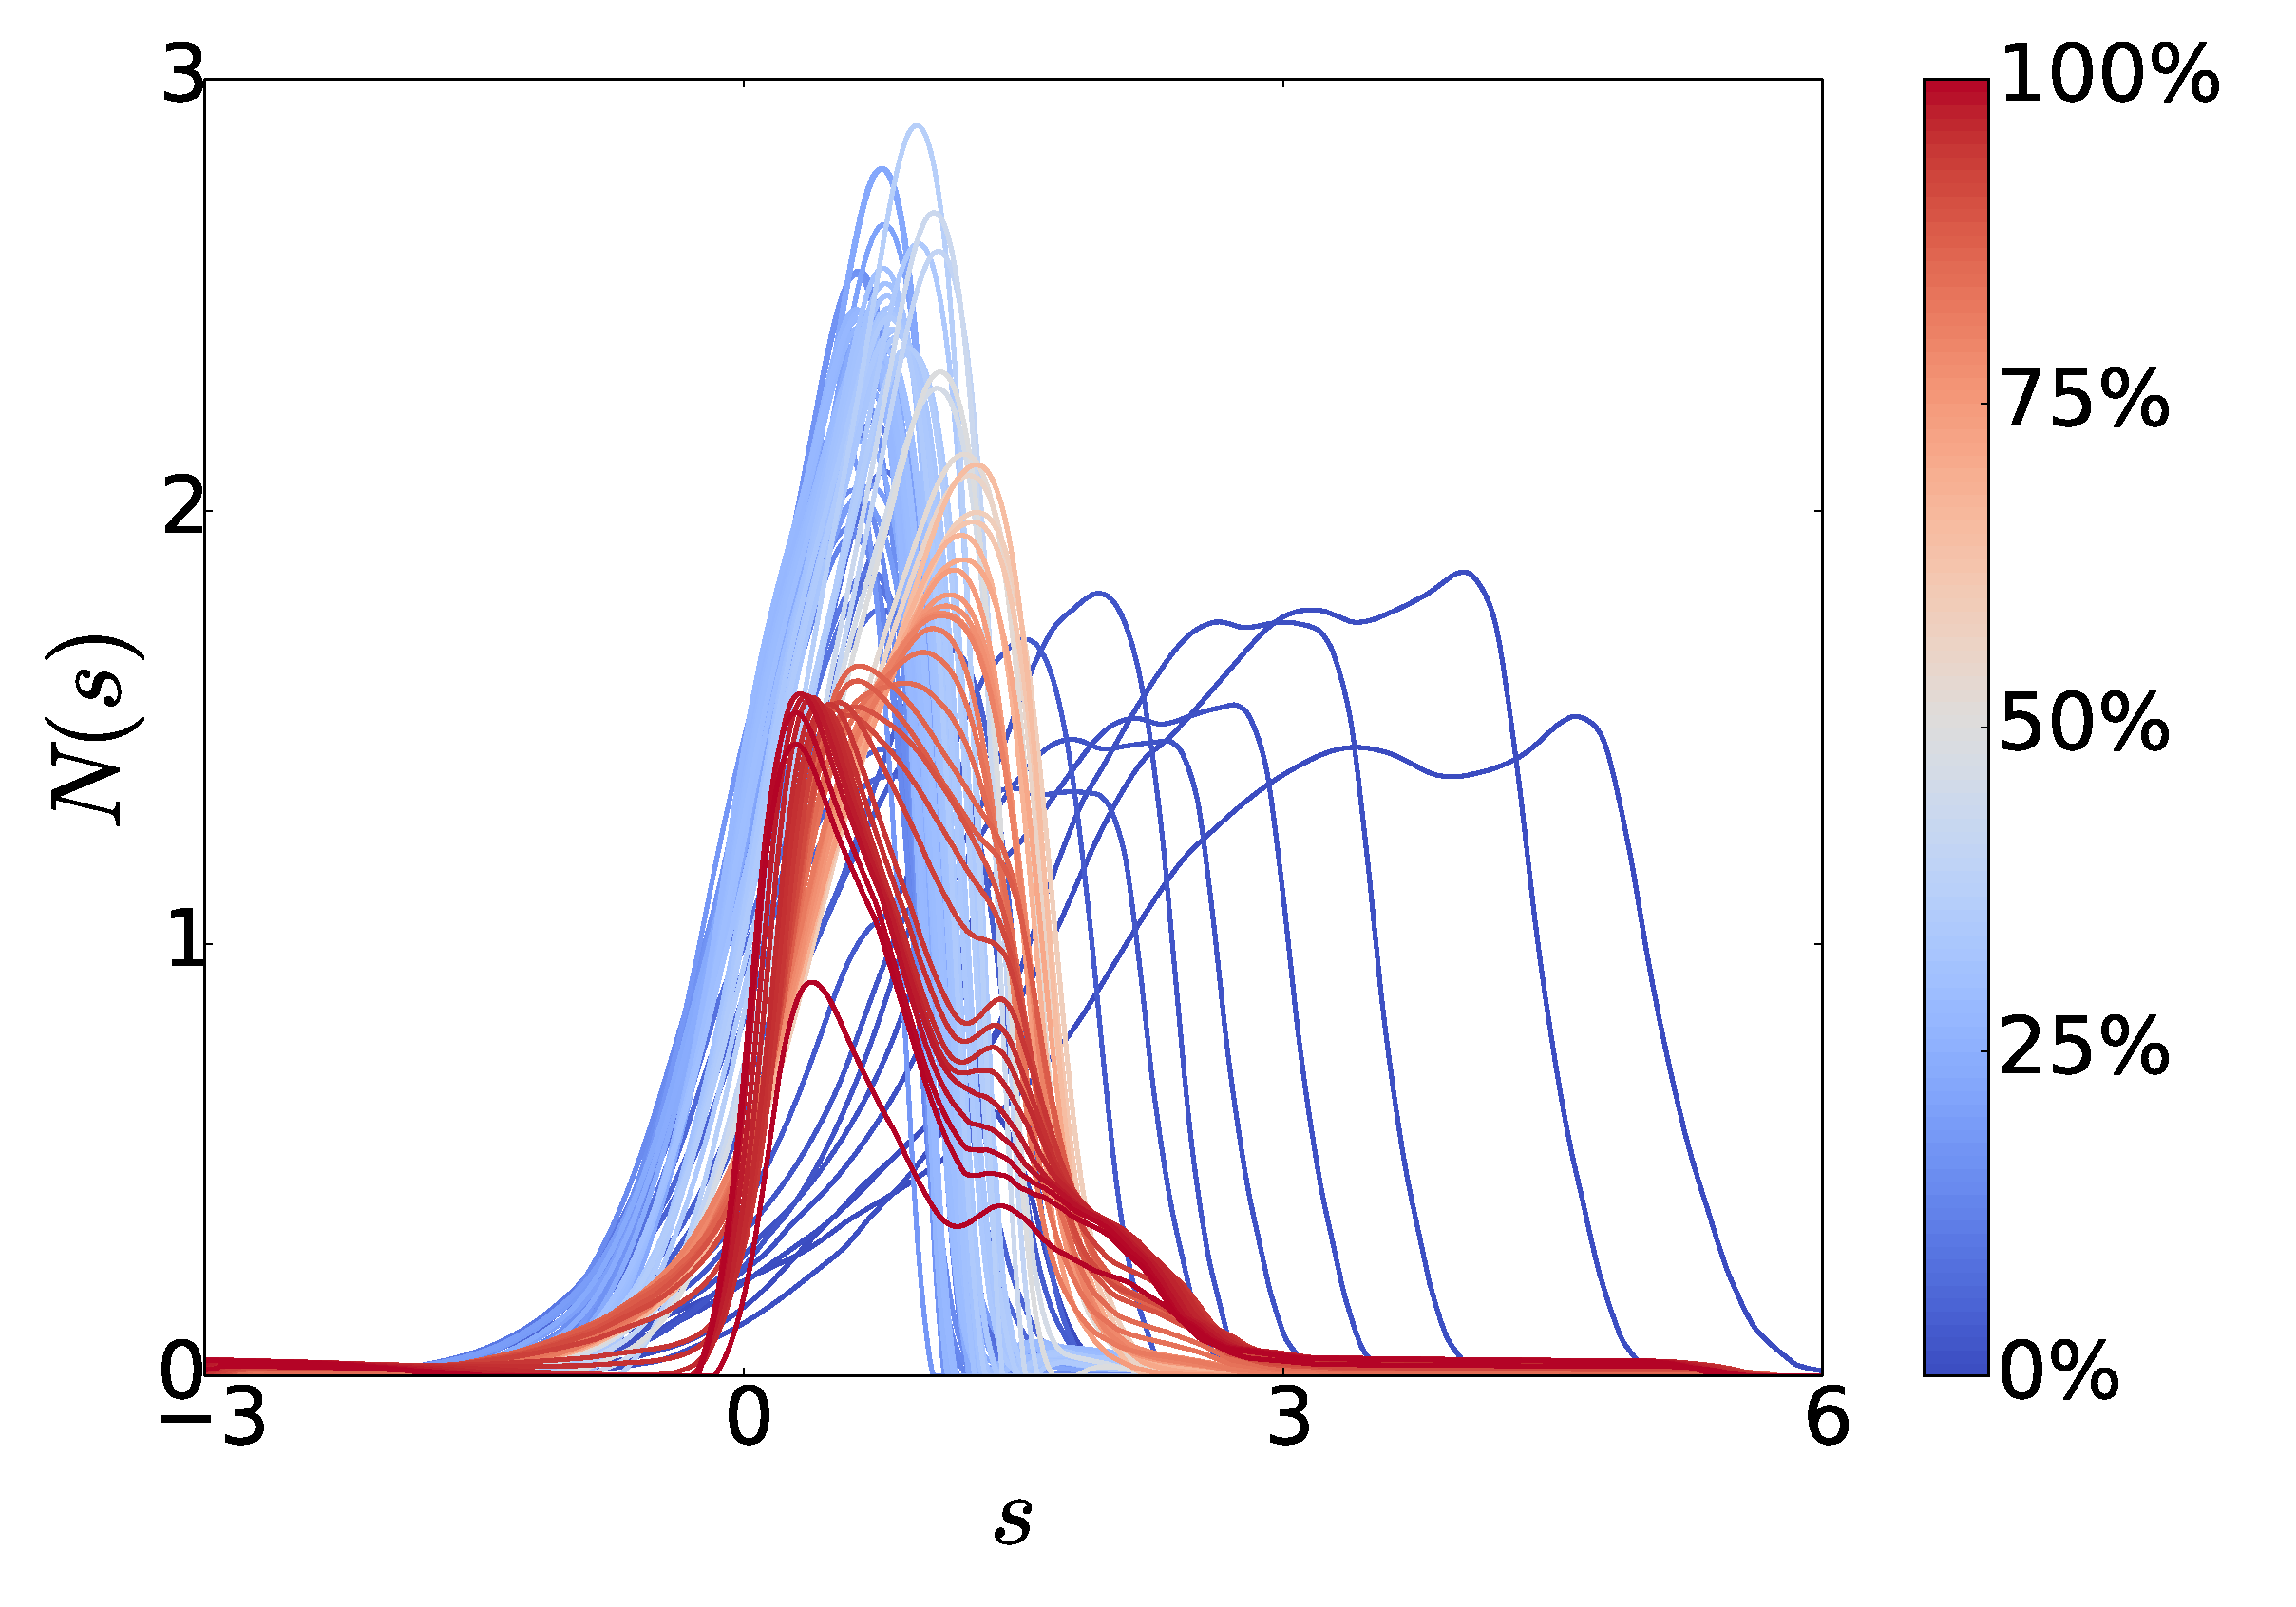
\includegraphics[width=1.25\textwidth]{PODReconstruction2} \\
    {\bf POD Reconstruction}
  \column{0.3\textwidth}
    \centering
    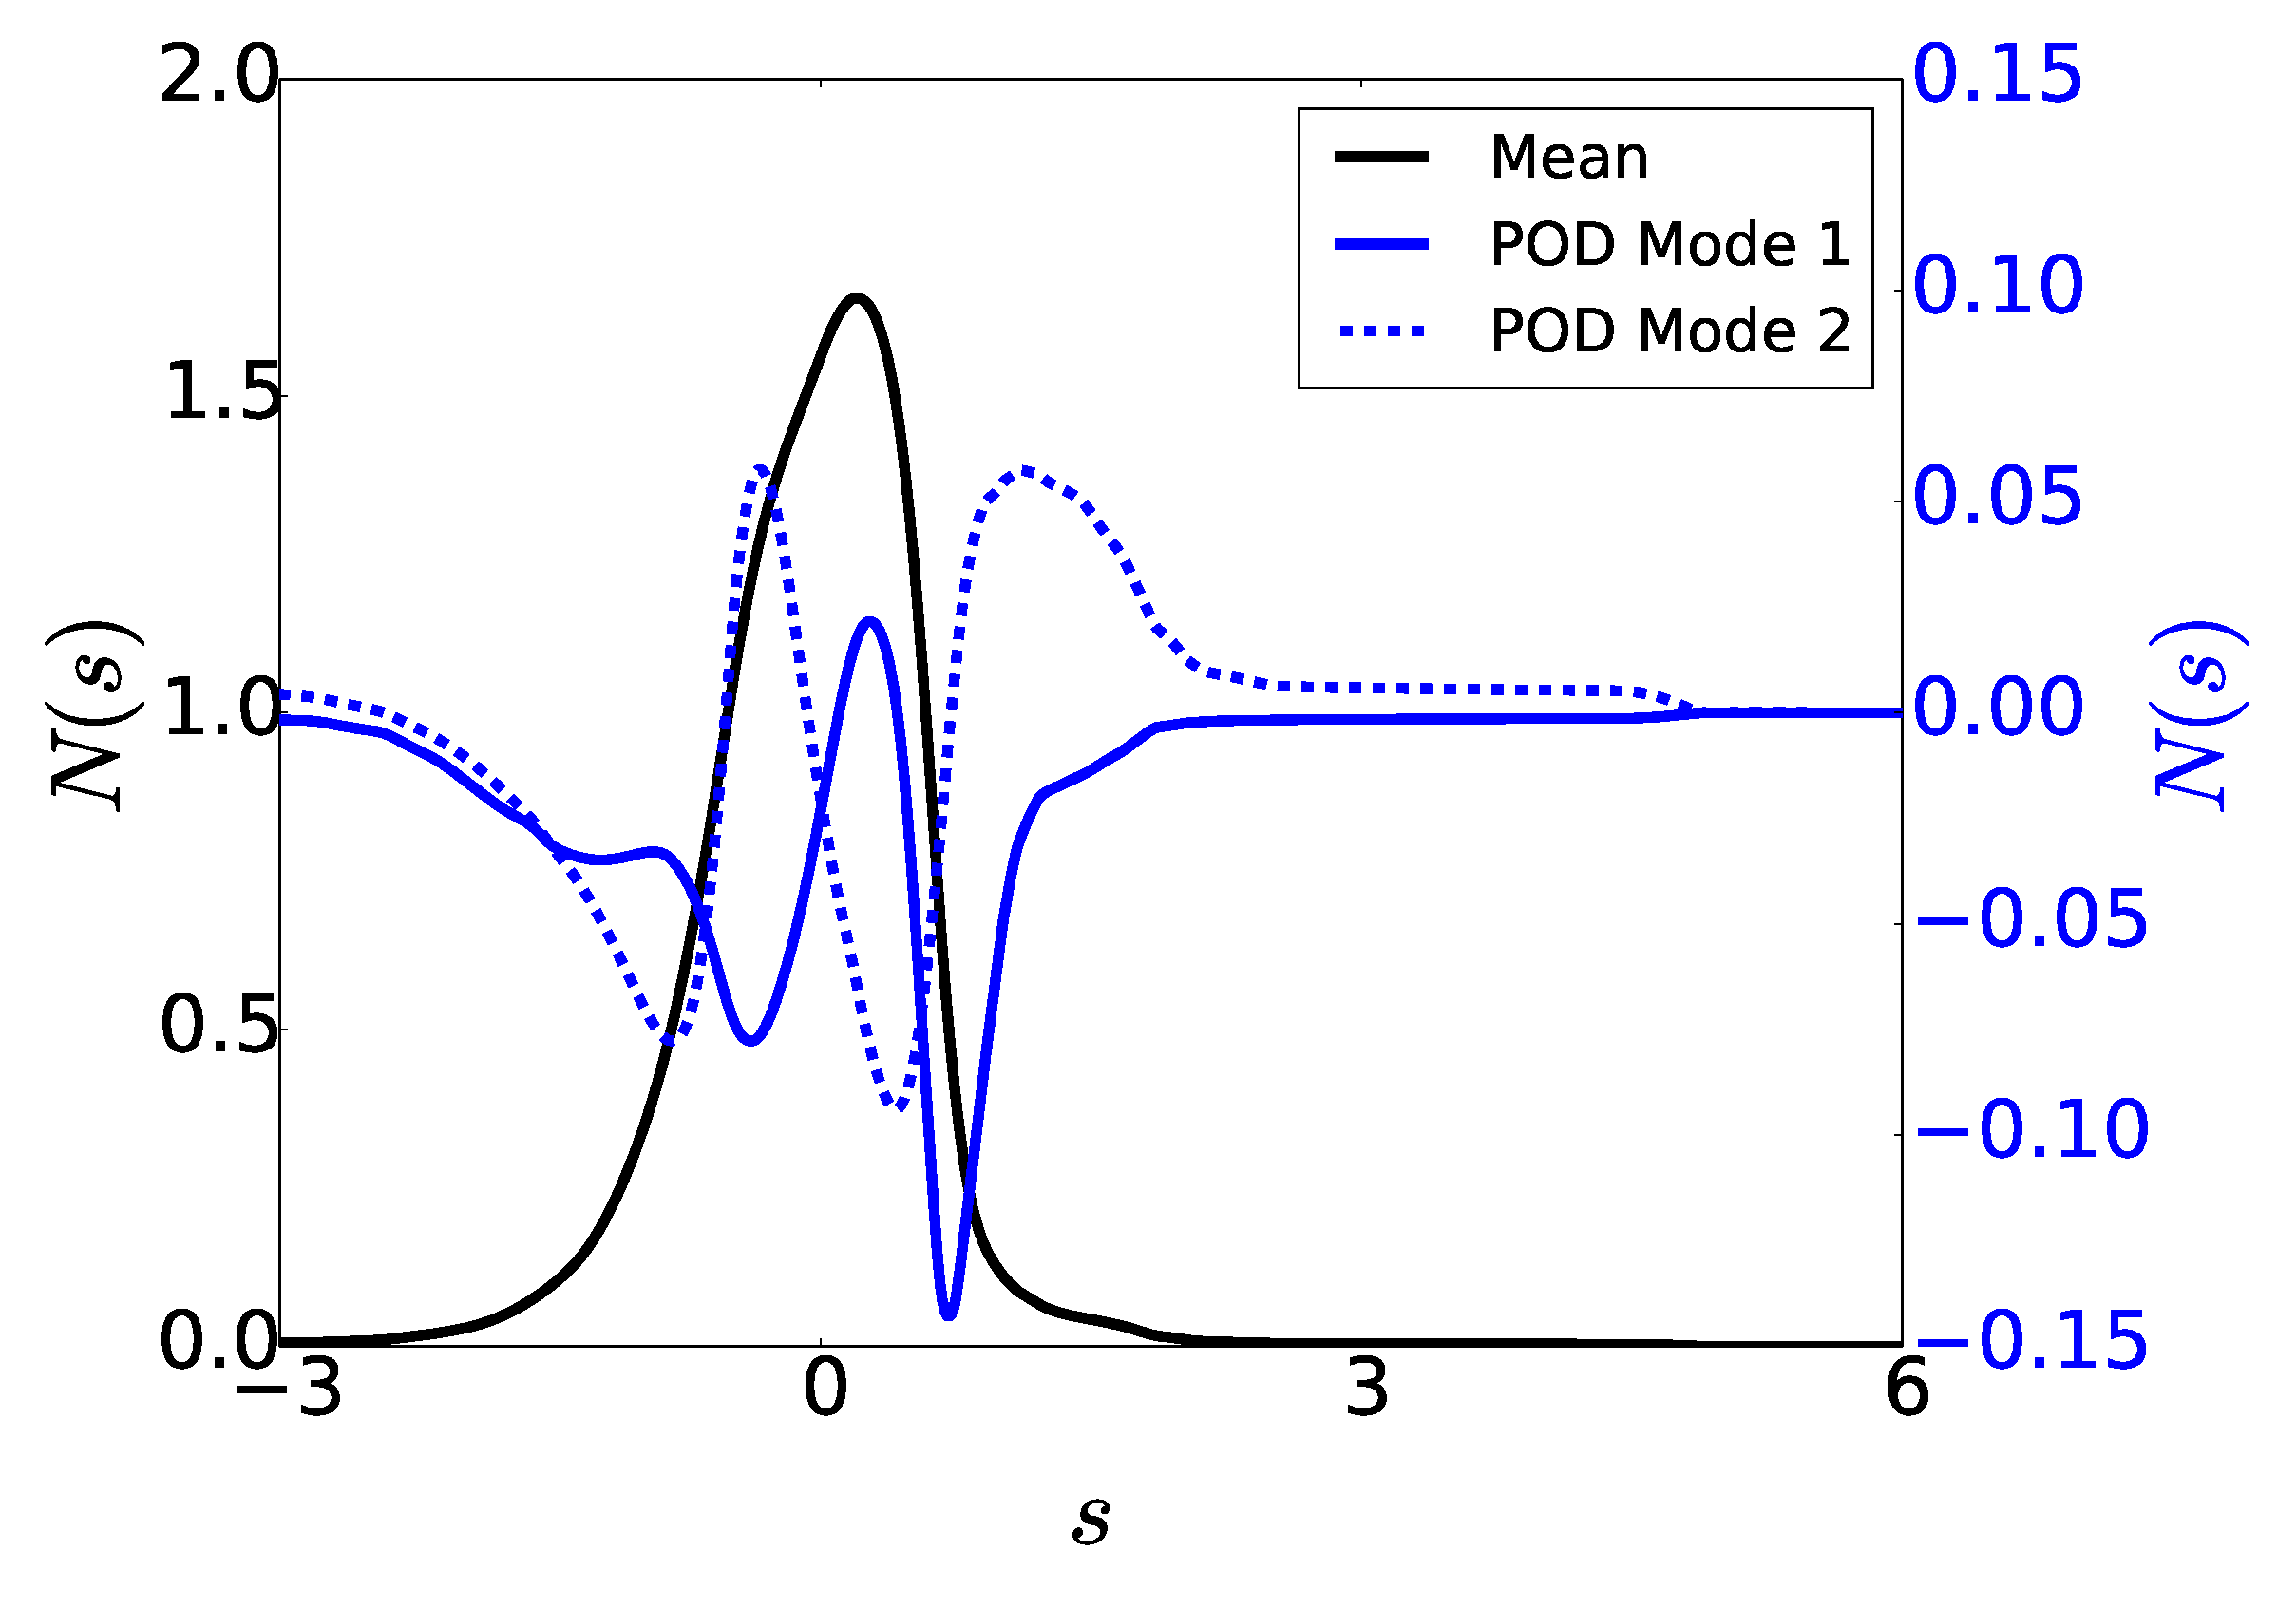
\includegraphics[width=1.25\textwidth]{PODModes} \\
    {\bf POD Modes}
\end{columns}
\vspace{1cm}
\begin{equation*}
N(s) = h \lbrace \bar{N}(as + b) + \sum_{i=1}^2 c_i \Phi_i(as + b)   \rbrace
\end{equation*}

\begin{itemize}
\item \emph{h, a, b} are scaling parameters
\item $c_1, c_2$ are POD coefficients
\item This collapses 100 different snapshots into 5 parameters
\end{itemize}
\end{frame}
\begin{frame}
\frametitle{5-Dimensional UQ Study}
\label{sec-3-3}


\begin{columns}[c]
  \column{0.5\textwidth}
    \centering
    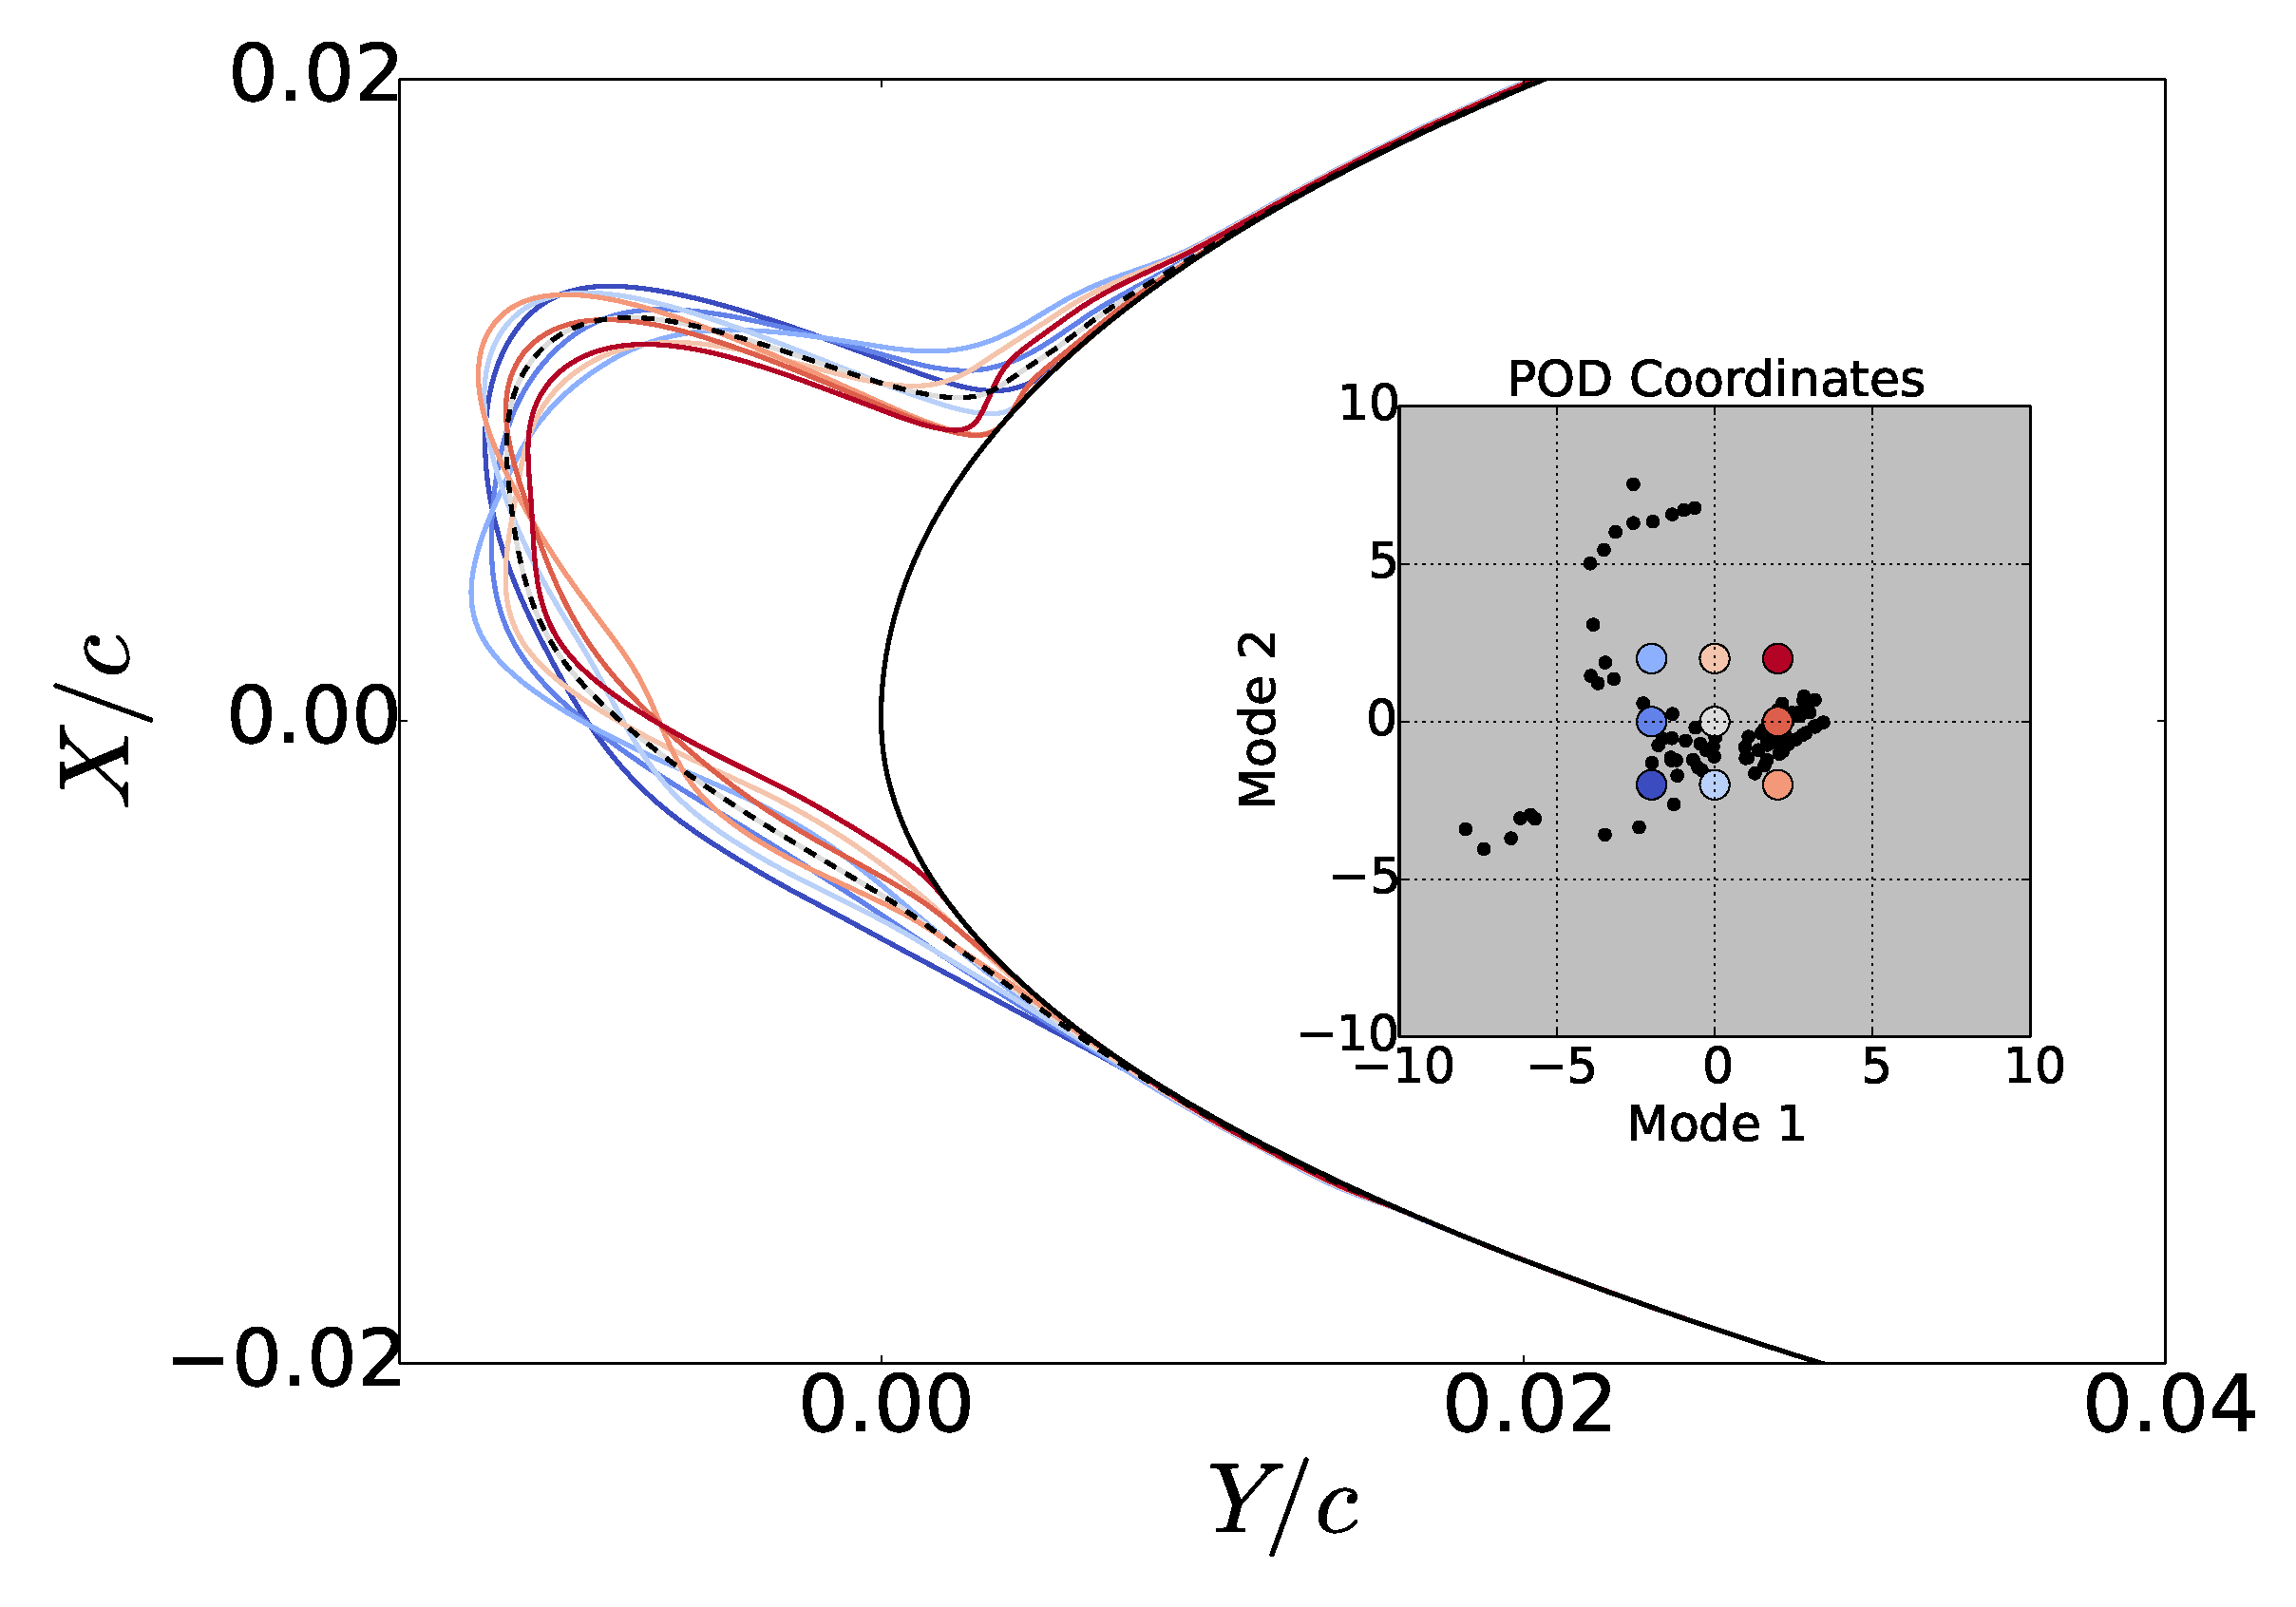
\includegraphics[width=.75\textwidth]{DifferentShapesPODModes} \\
    \bf{POD Modes} \\
    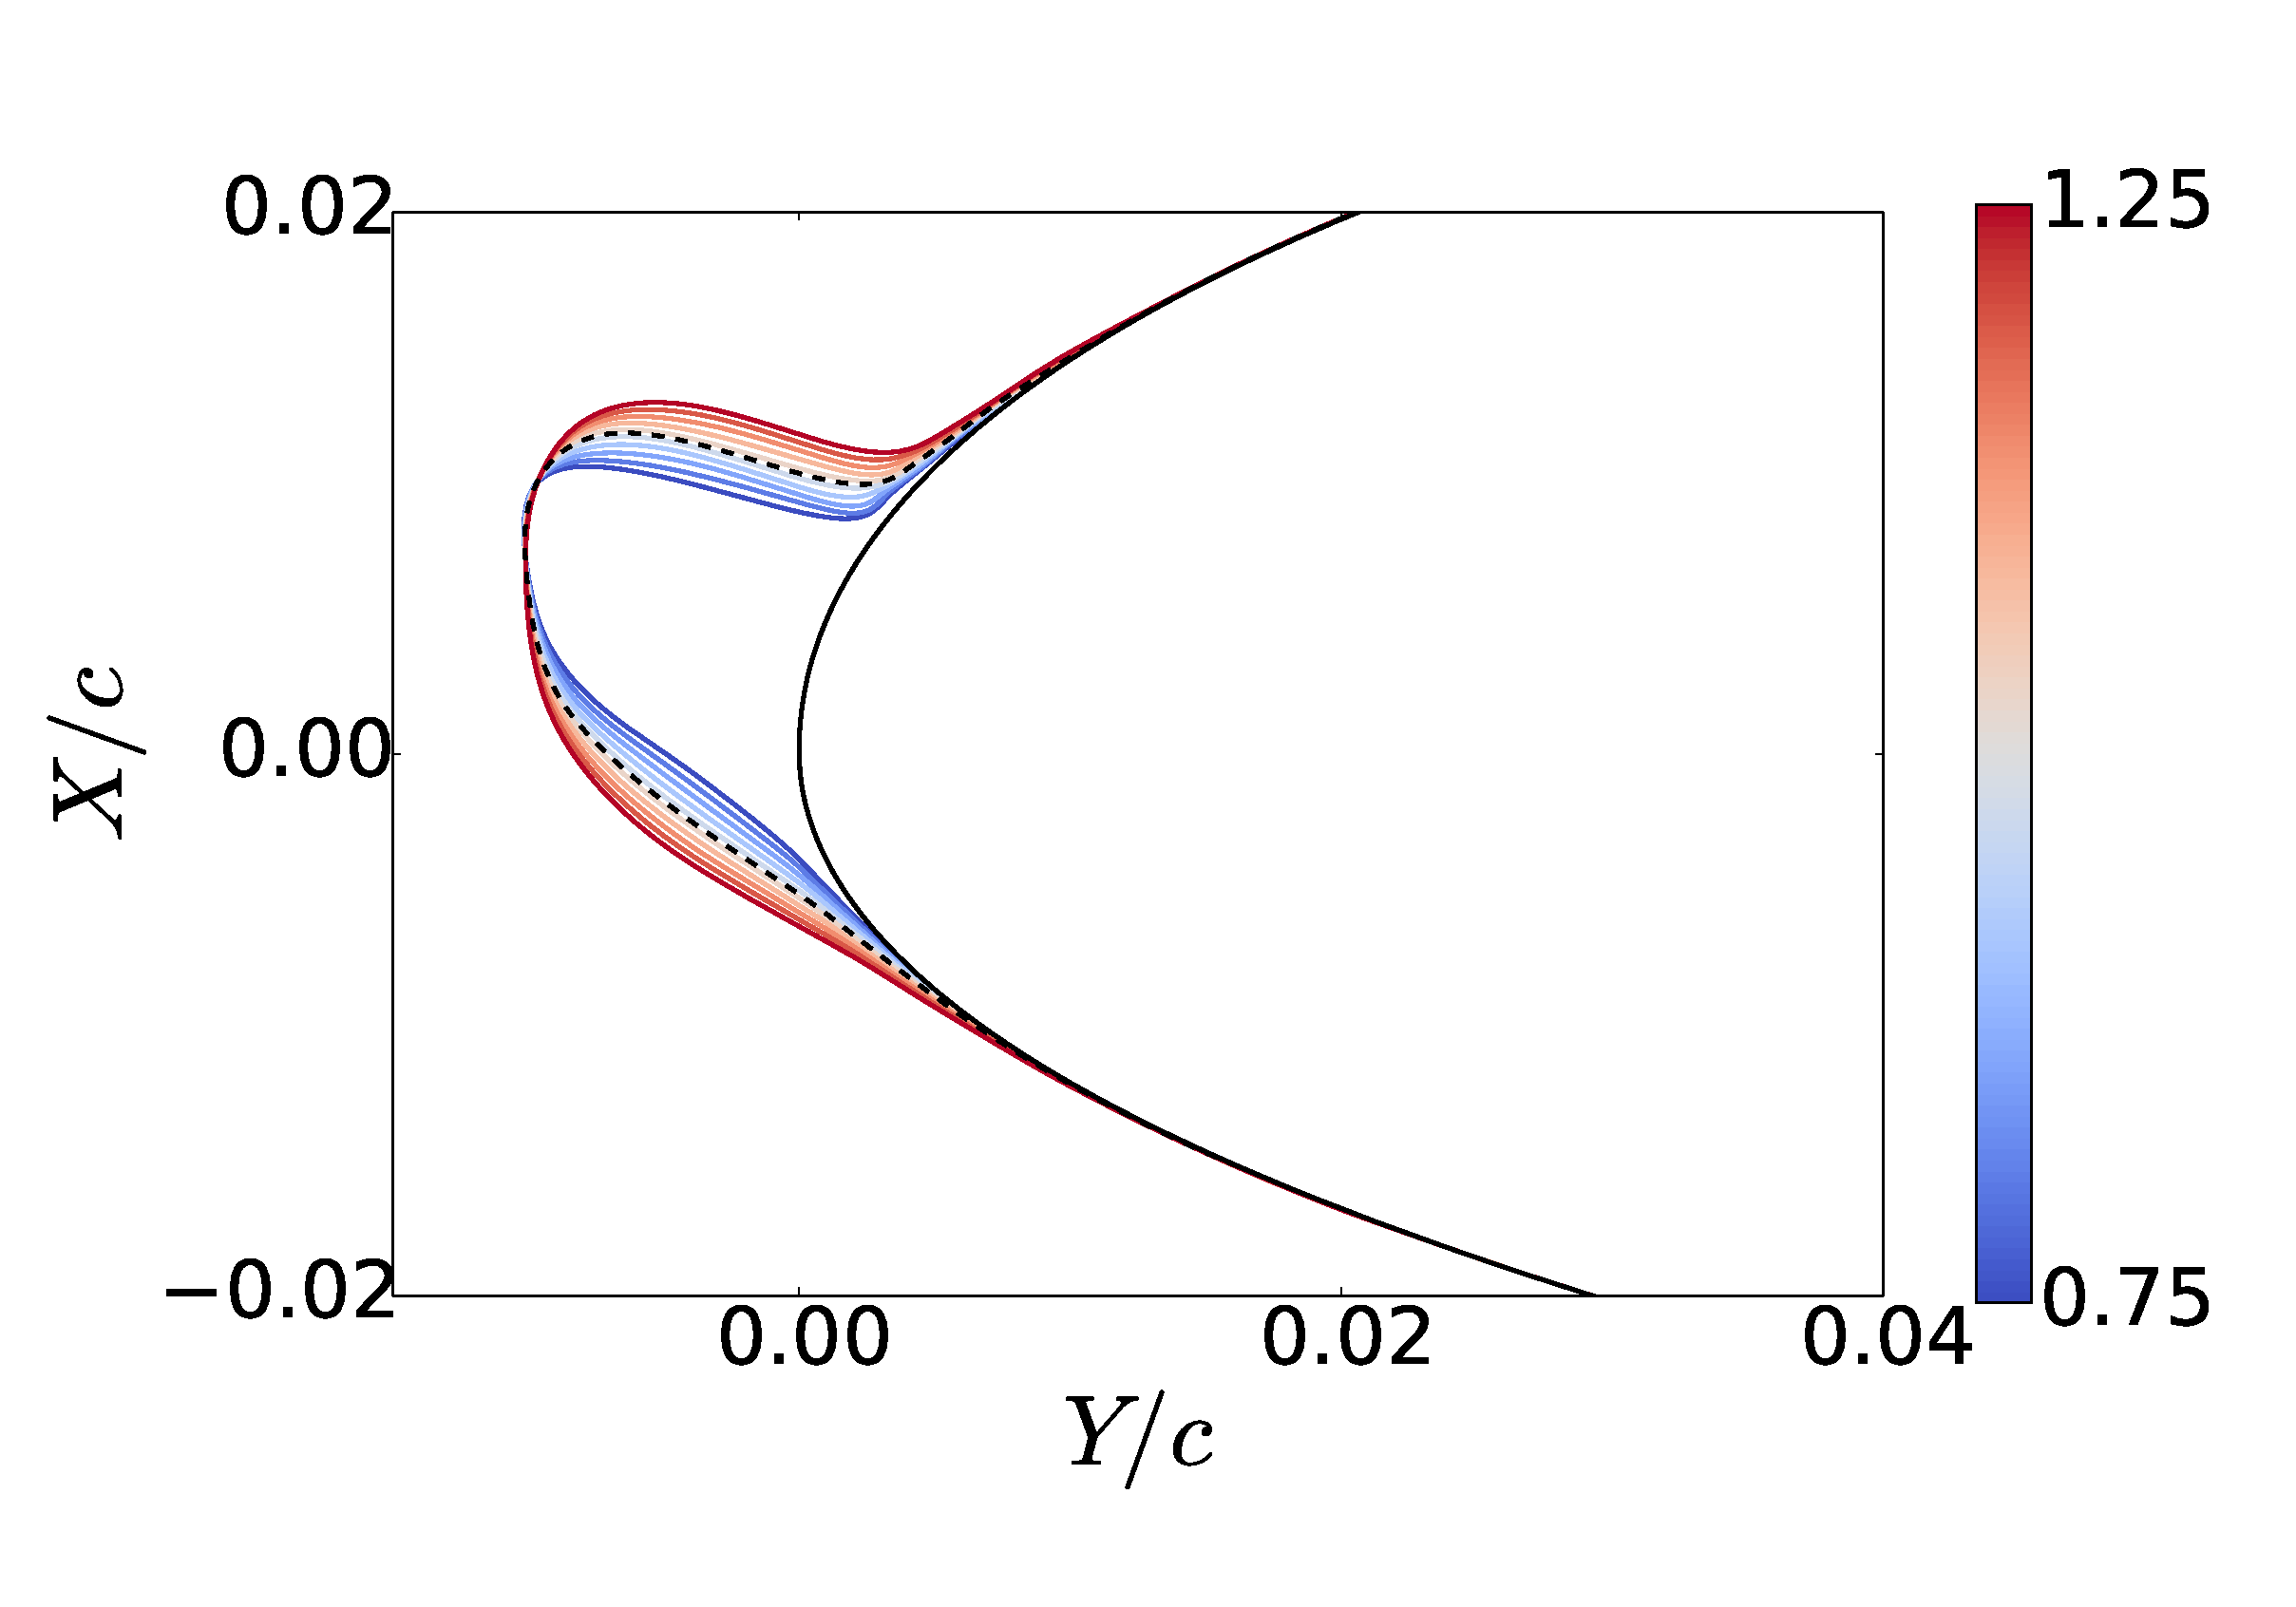
\includegraphics[width=.75\textwidth]{DifferentShapesWidth} \\
    \bf{Width}
  \column{0.5\textwidth}
    \centering
    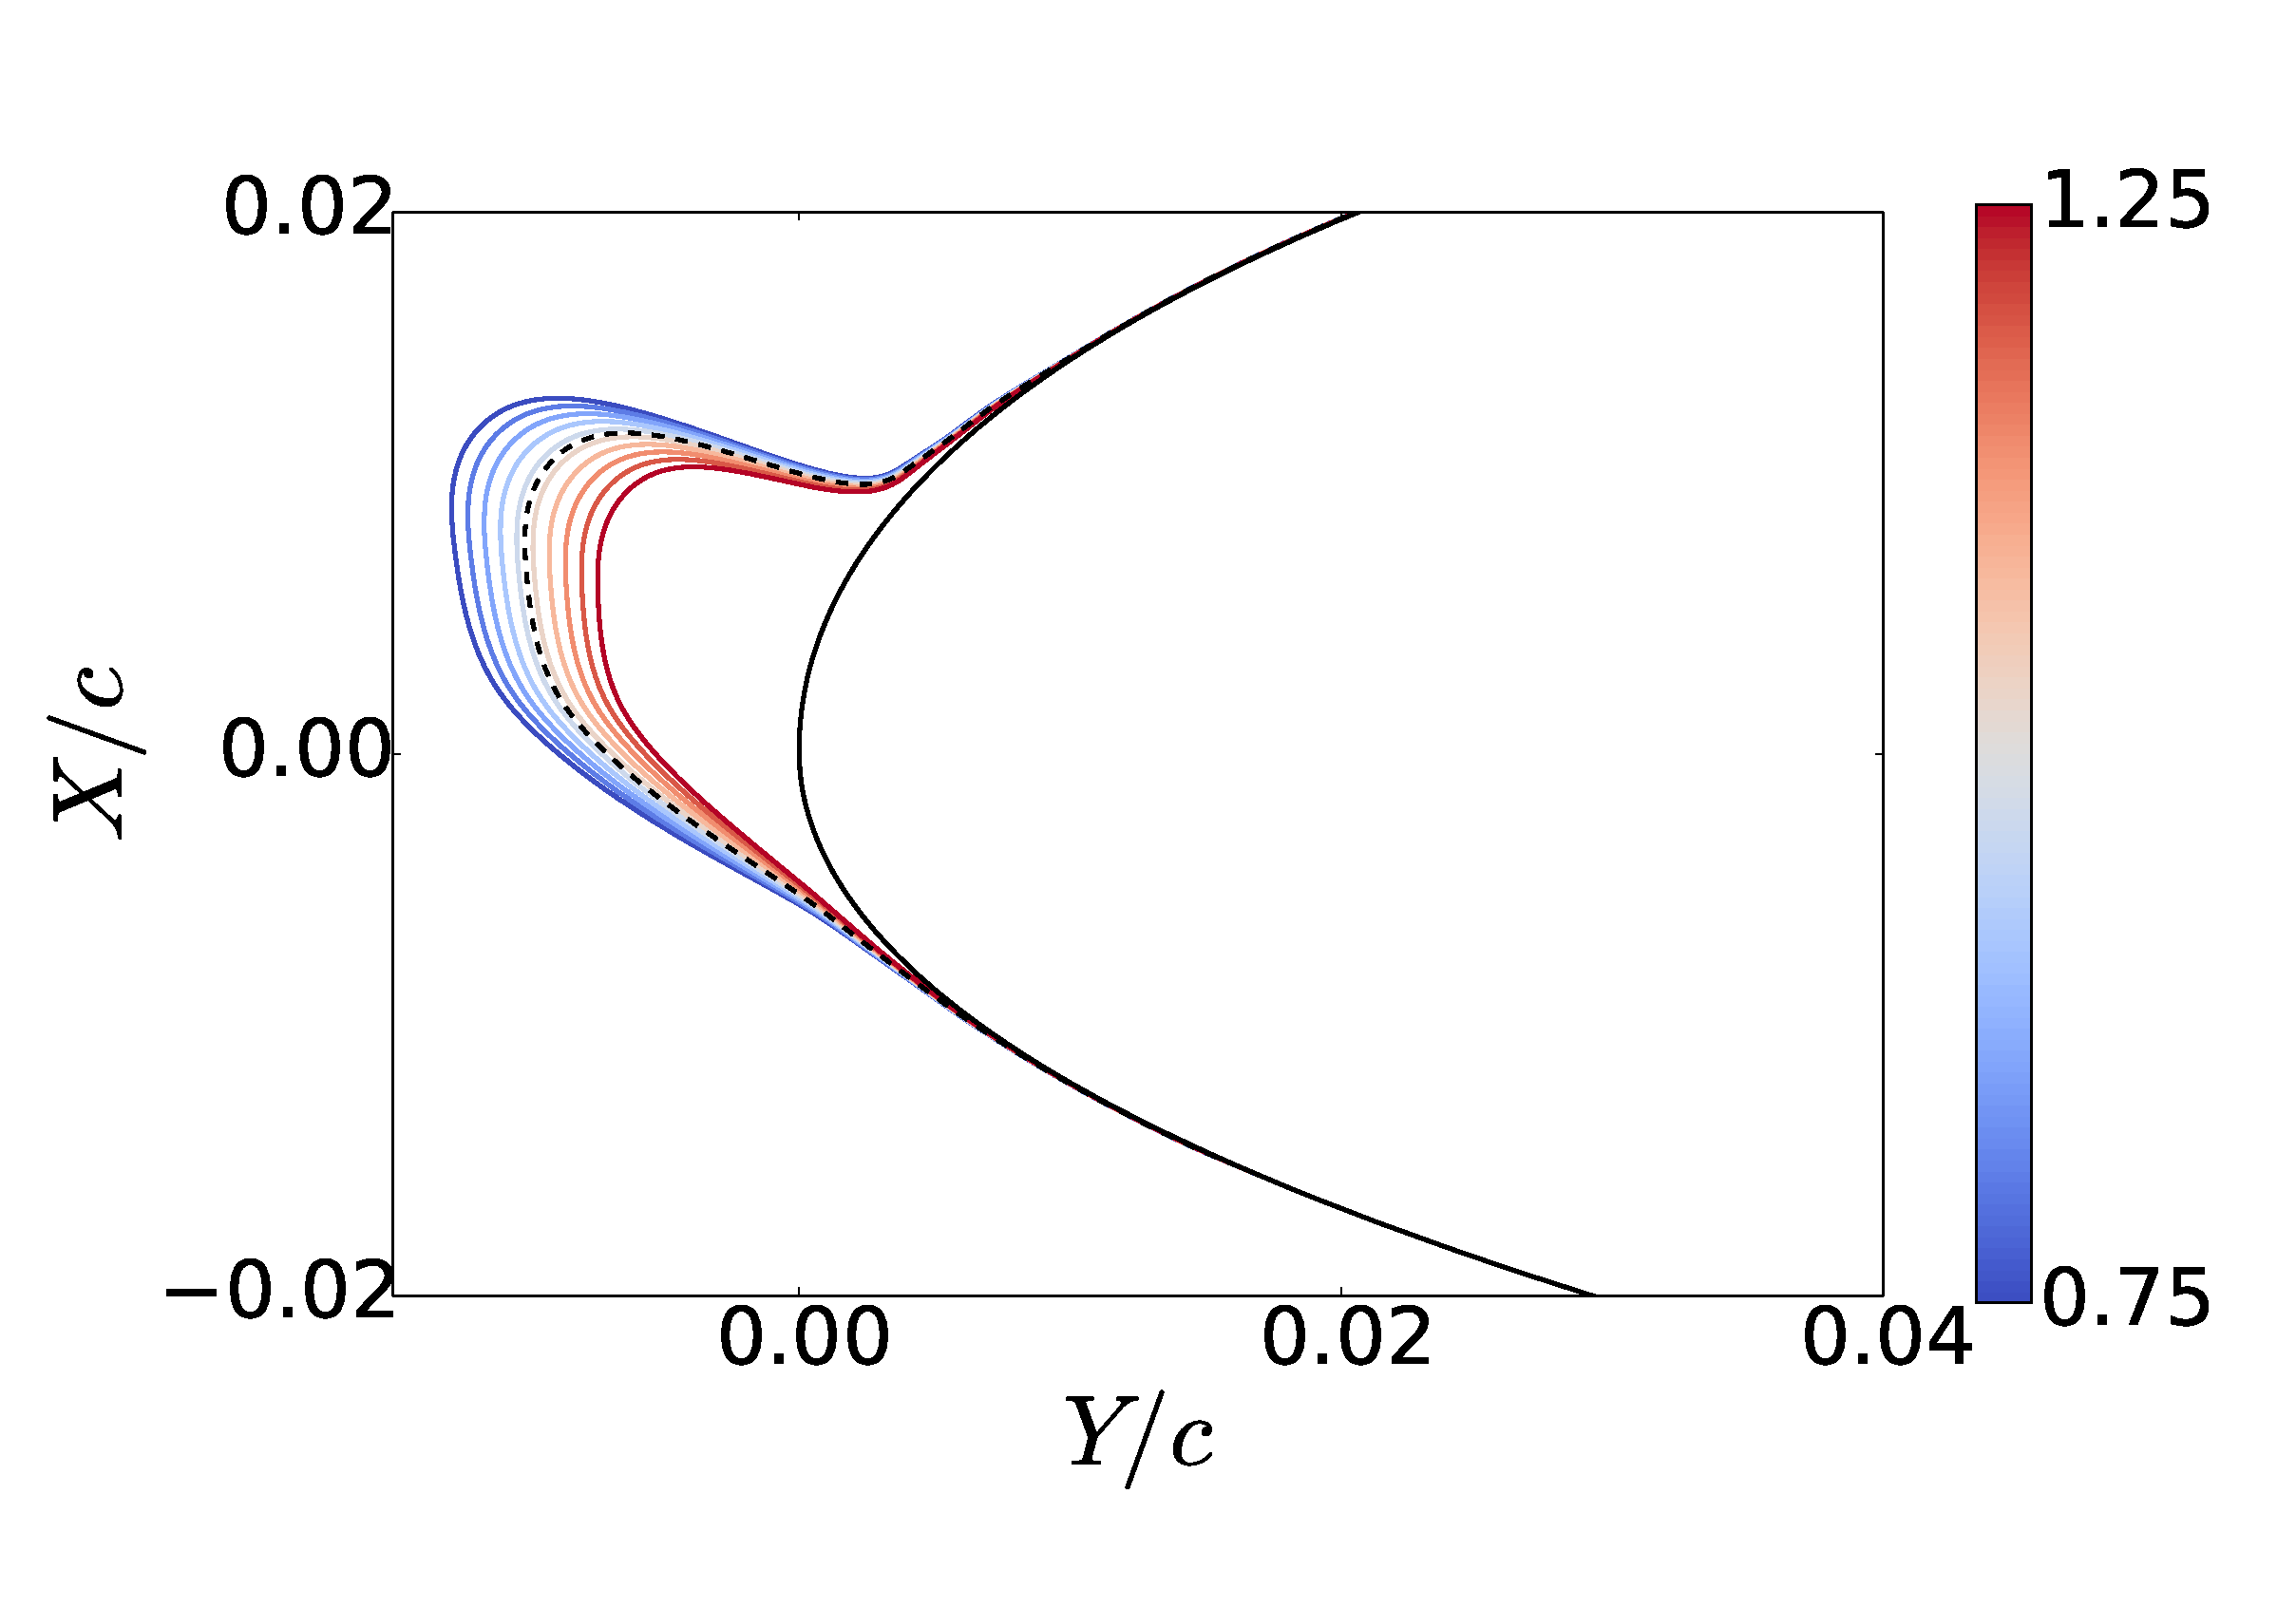
\includegraphics[width=.75\textwidth]{DifferentShapesHeight} \\
    {\bf Height} \\
    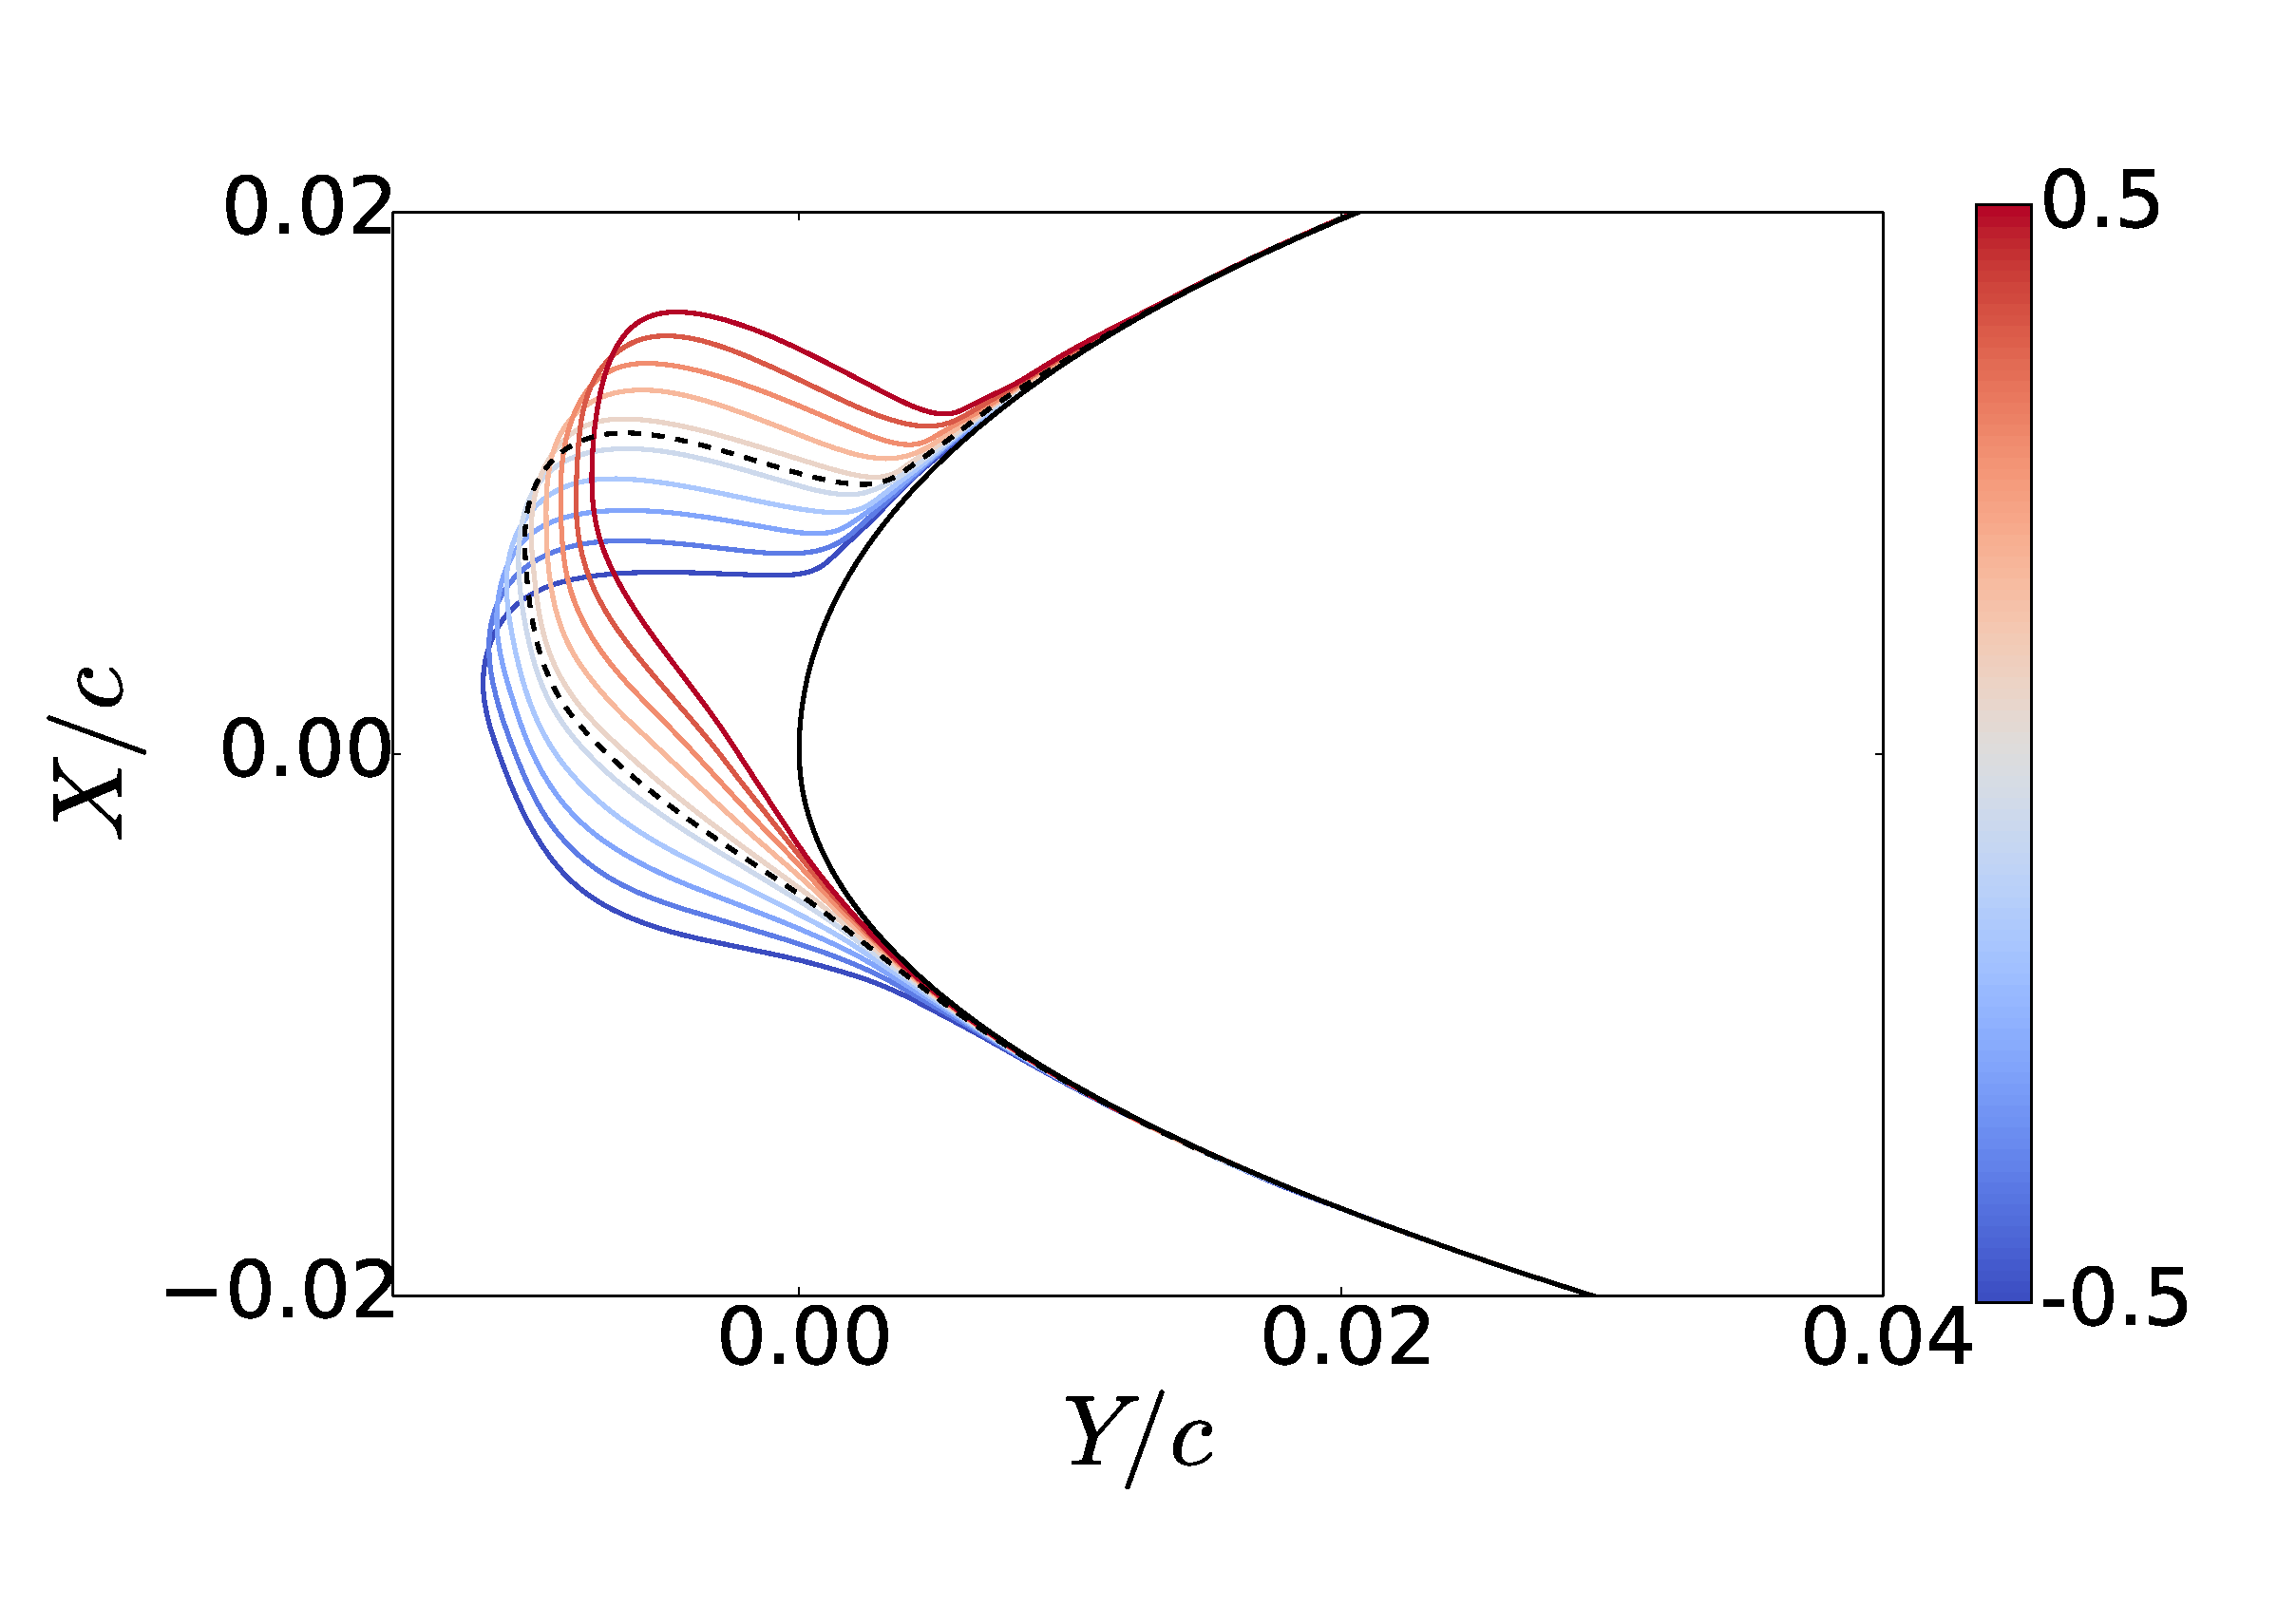
\includegraphics[width=.75\textwidth]{DifferentShapesPosition} \\
    {\bf Position}    
\end{columns}

\begin{itemize}
\item 2 POD coefficients (\emph{shape}) + width, height, position parameters (\emph{scaling})
\end{itemize}
\end{frame}
\begin{frame}
\frametitle{Statistics}
\label{sec-3-4}


\begin{columns}[c]
  \column{0.37\textwidth}
    \centering
    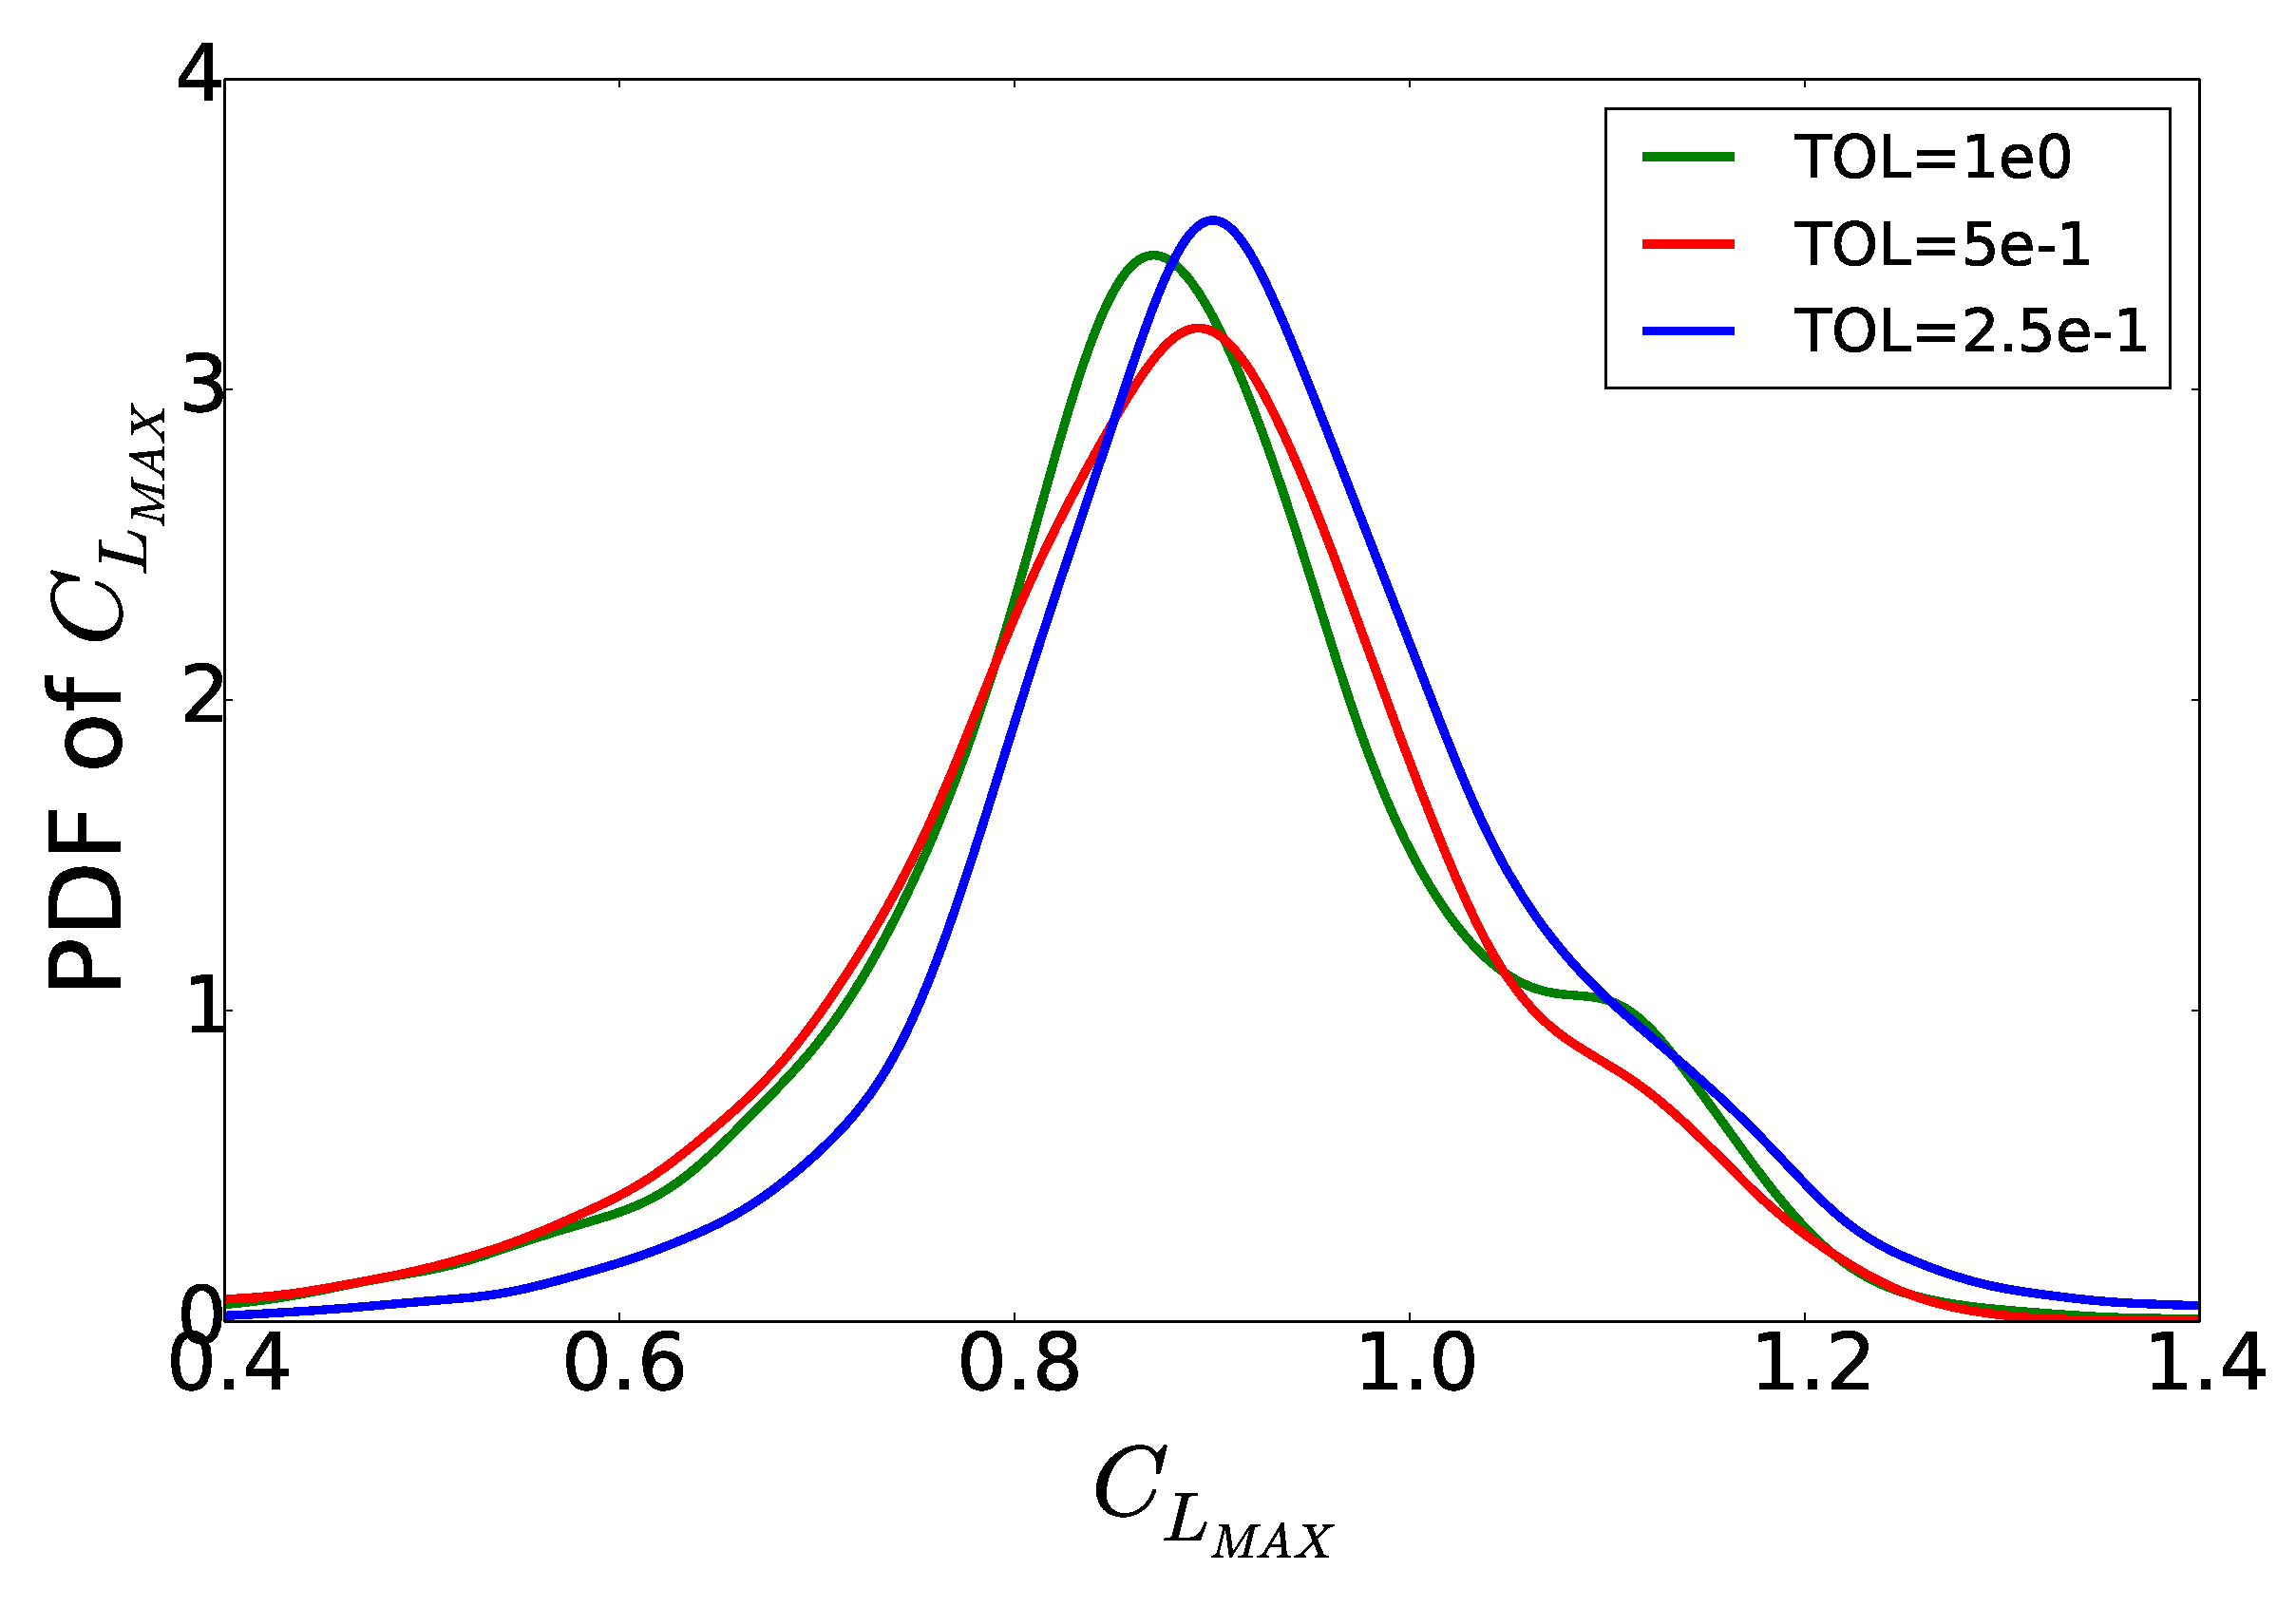
\includegraphics[width=1\textwidth]{PDFCLMAX} \\
    $\bm{C_L}$ {\bf Statistics}
  \column{0.37\textwidth}
    \centering
    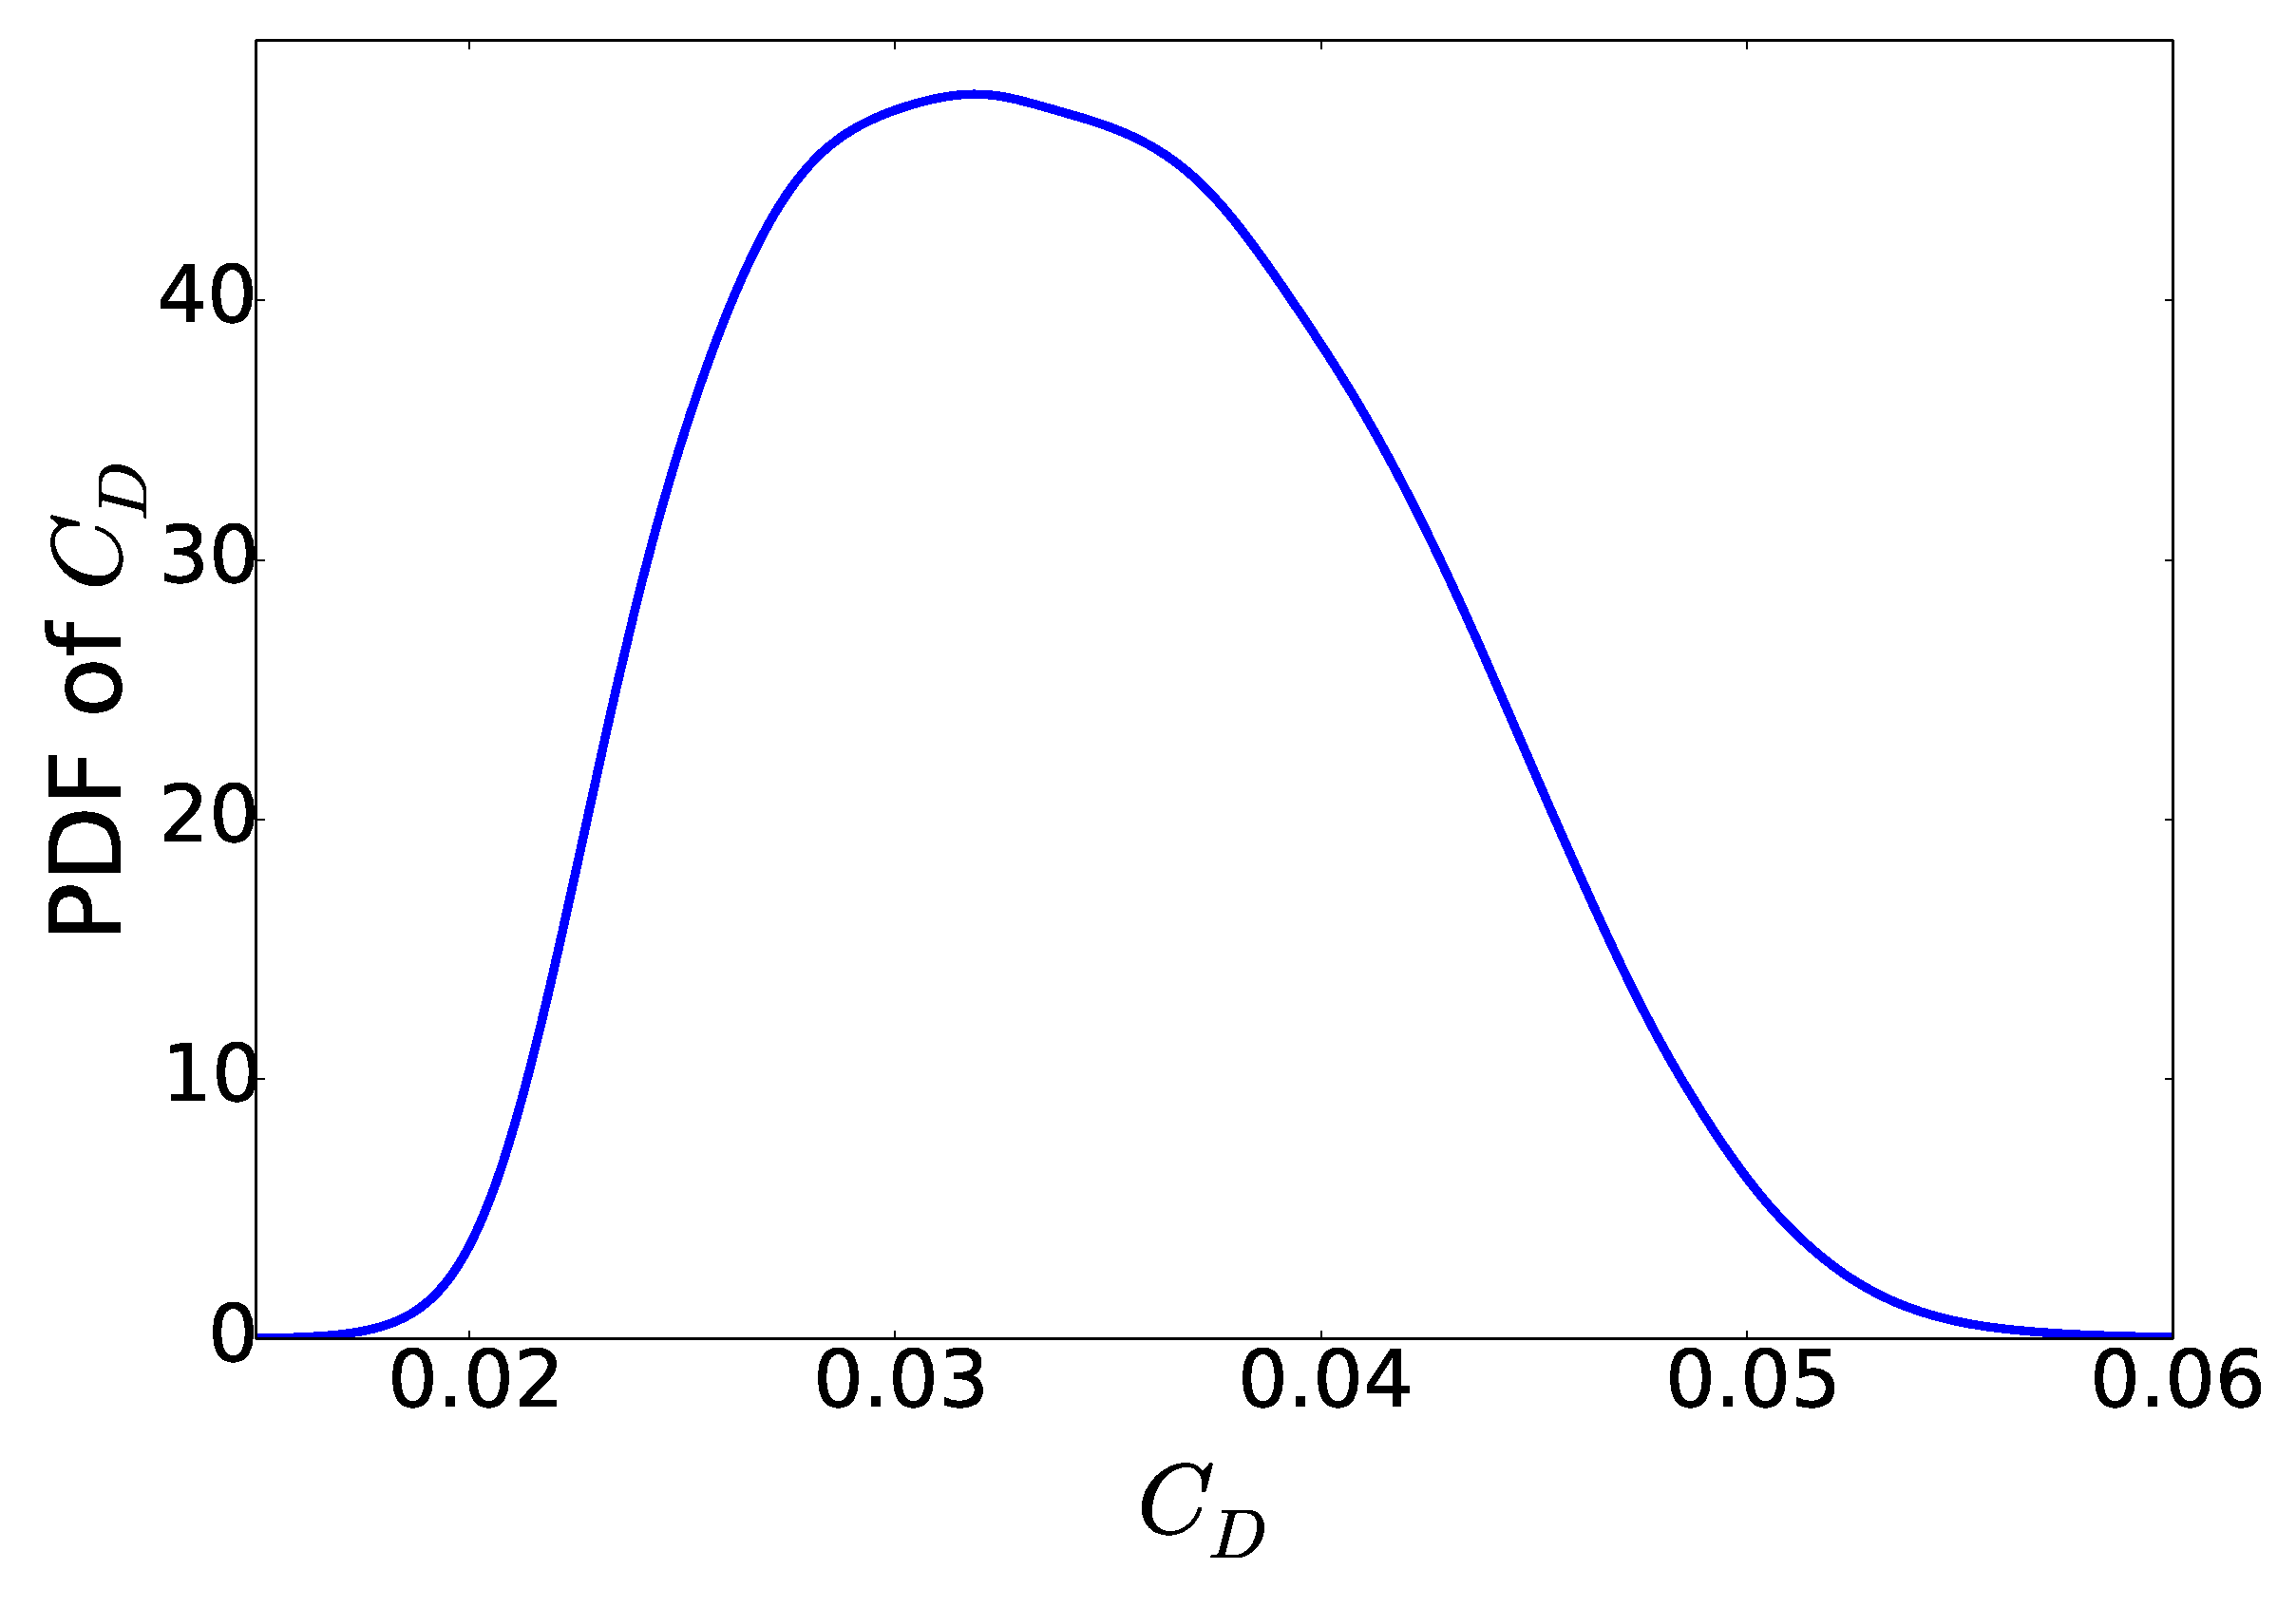
\includegraphics[width=1\textwidth]{PDFCDMAX} \\
    $\bm{C_D}$ {\bf Statistics}
\end{columns}



\begin{center}
\begin{tabular}{lrrrrr}
            &  Width  &  Position  &  Height  &  POD 1  &  POD 2  \\
\hline
 T ($C_L$)  &   0.03  &      0.69  &    0.15  &   0.11  &   0.14  \\
\end{tabular}
\end{center}



\begin{itemize}
\item Our surrogate is an explicit polynomial function of the input
  variables, making statistical inference easy/quick
\item PCE surrogate computed using 1,103 sparse grid points
\item Sobol index $T_i = \frac{\mathbb{E}\left[ Var\left(
  Y|Z_{-i}\right)\right]}{Var\left( Y\right)}$ is a measure of how much
  $Z_i$ contributes to the total variance of $Y(\bv{Z})$
\item For our parameter ranges, position perturbation accounts for most of
  the statistical variation
\end{itemize}
\end{frame}
\begin{frame}
\frametitle{Statistical Inference}
\label{sec-3-5}


\begin{itemize}
\item Analyze statistical clustering of horns that produce bottom and top
  $10\%$ of $C_L$ variation
\end{itemize}

\begin{columns}[c]
  \column{0.40\textwidth}
    \centering
    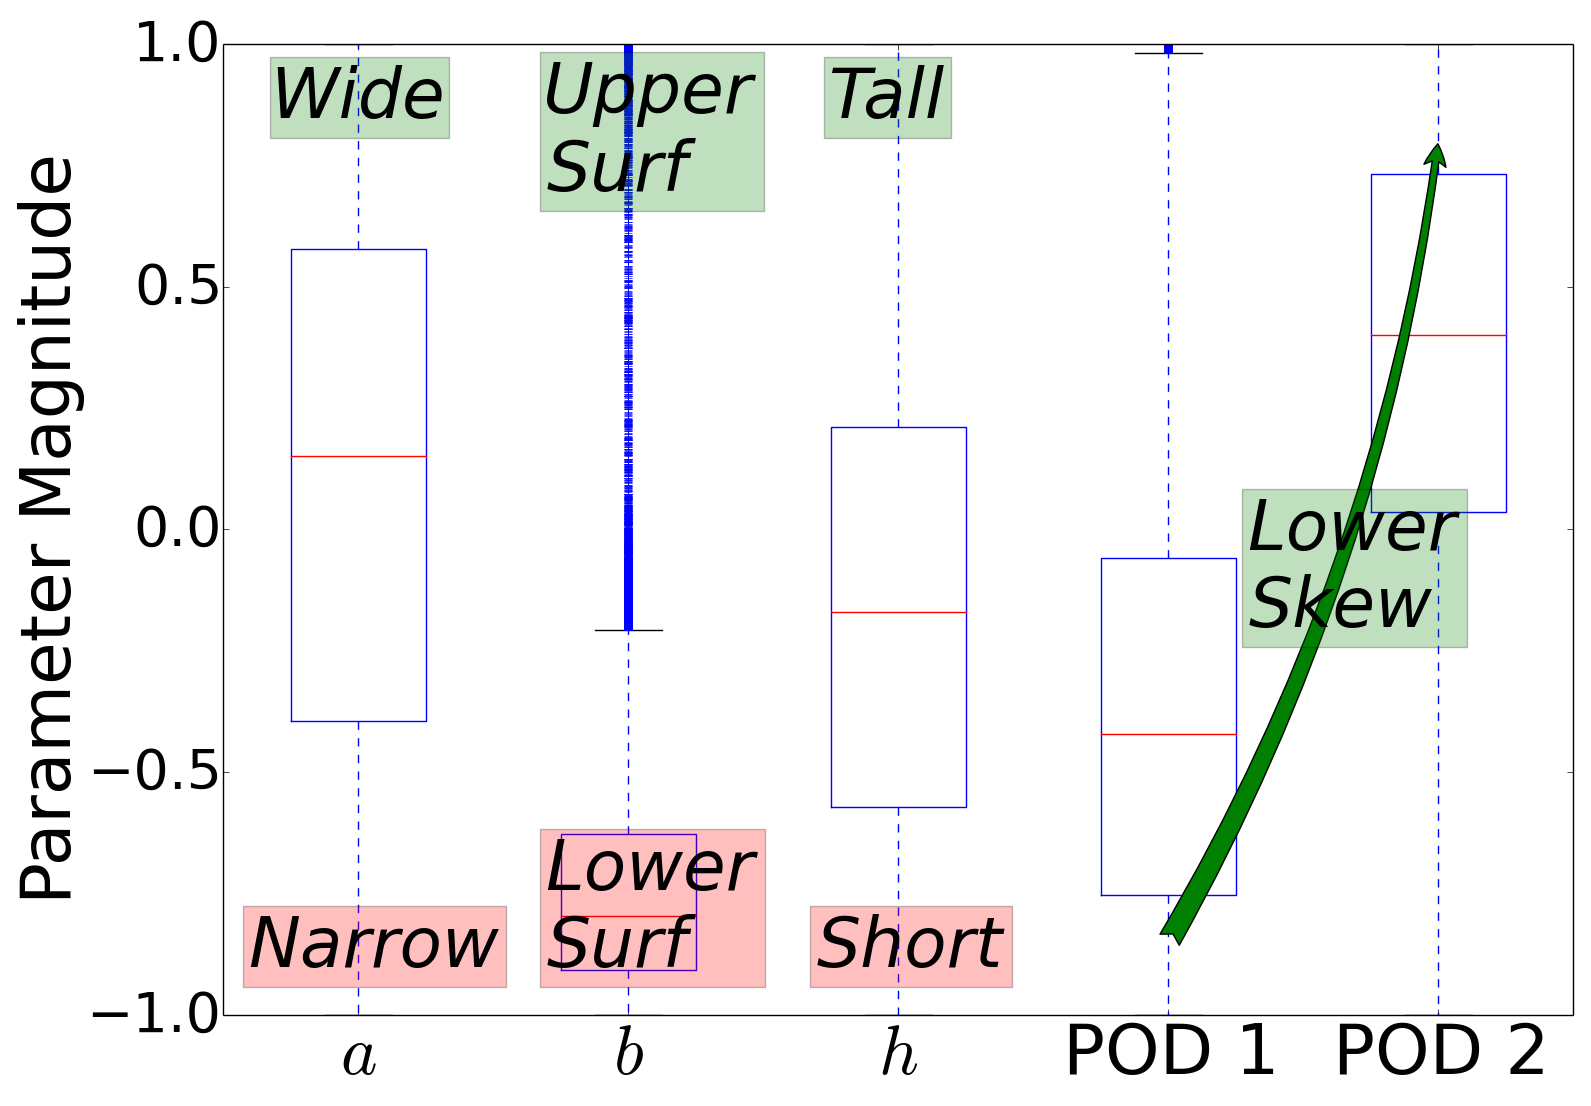
\includegraphics[width=1\textwidth]{GoodHornParamLocs.png} \\
    {\bf Favorable Horns}
    \begin{itemize}
      \item Wider/rounded
      \item Lower surface
      \item Shorter
      \item Gentle downward skew
    \end{itemize}
  \column{0.40\textwidth}
    \centering
    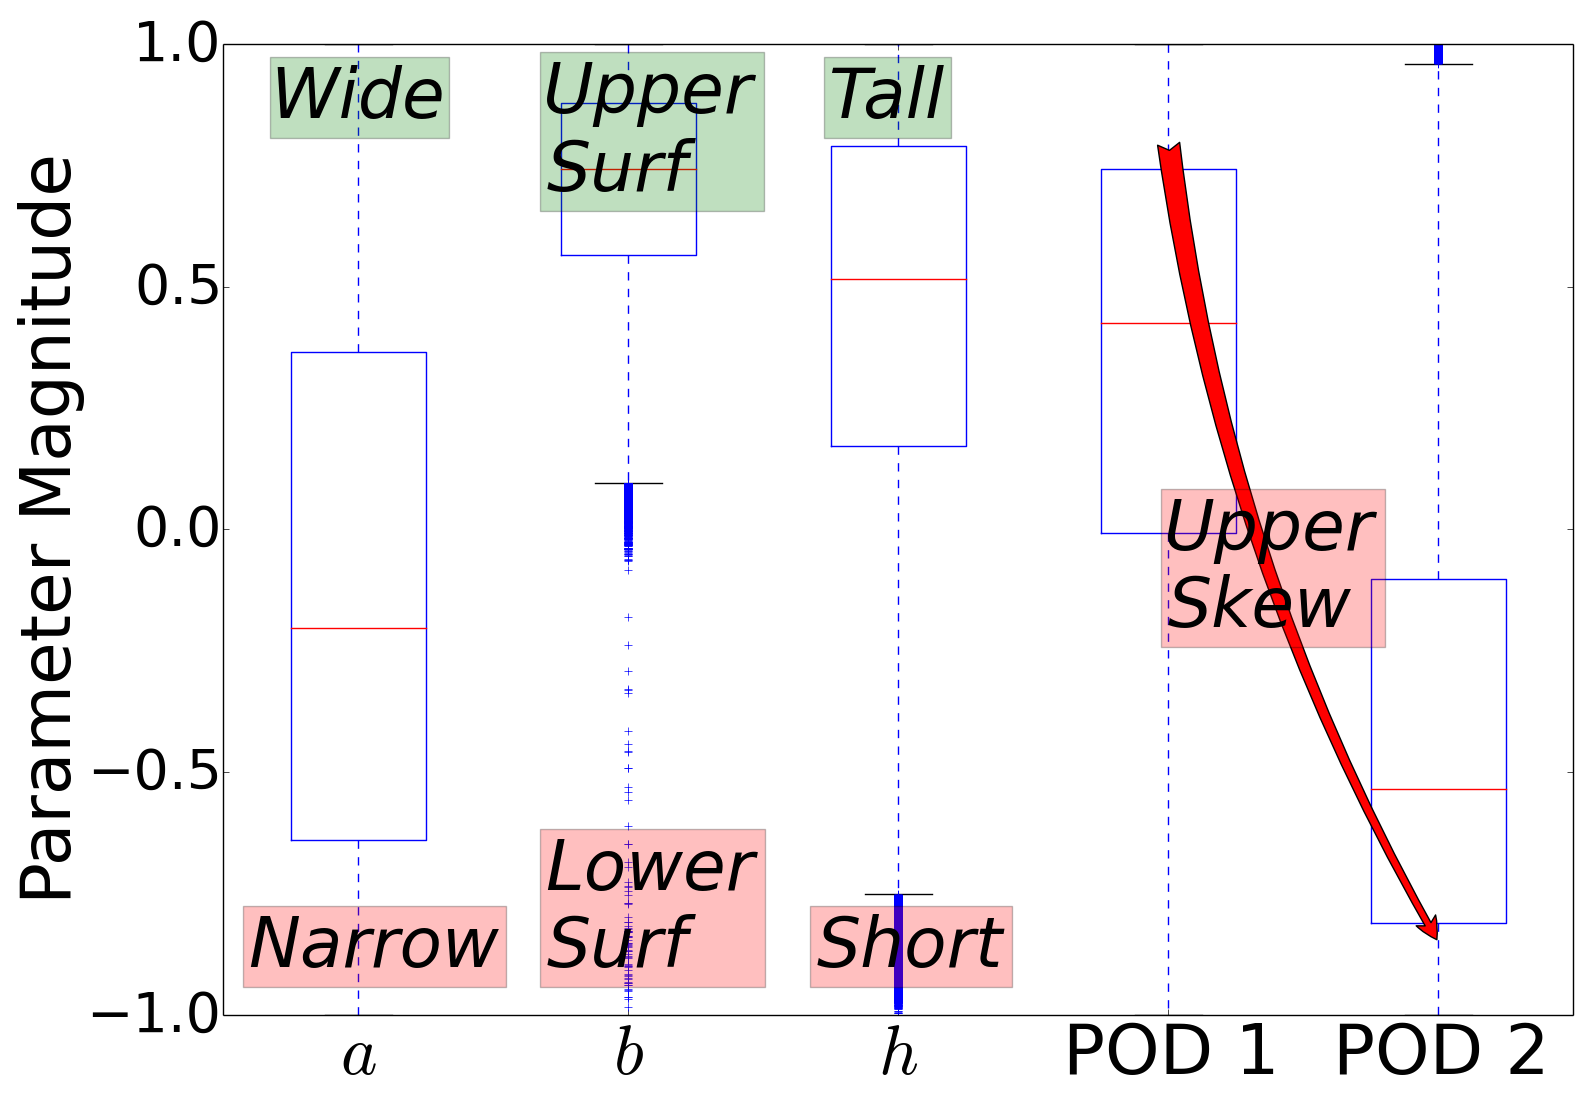
\includegraphics[width=1\textwidth]{BadHornParamLocs.png} \\
    {\bf Unfavorable Horns}
    \begin{itemize}
      \item Sharper/narrower
      \item Upper surface
      \item Taller
      \item Sharp, upper skew shape
    \end{itemize}
\end{columns}
\end{frame}
\begin{frame}
\frametitle{Flow Solutions}
\label{sec-3-6}


\begin{columns}[c]
  \column{0.30\textwidth}
    \centering
    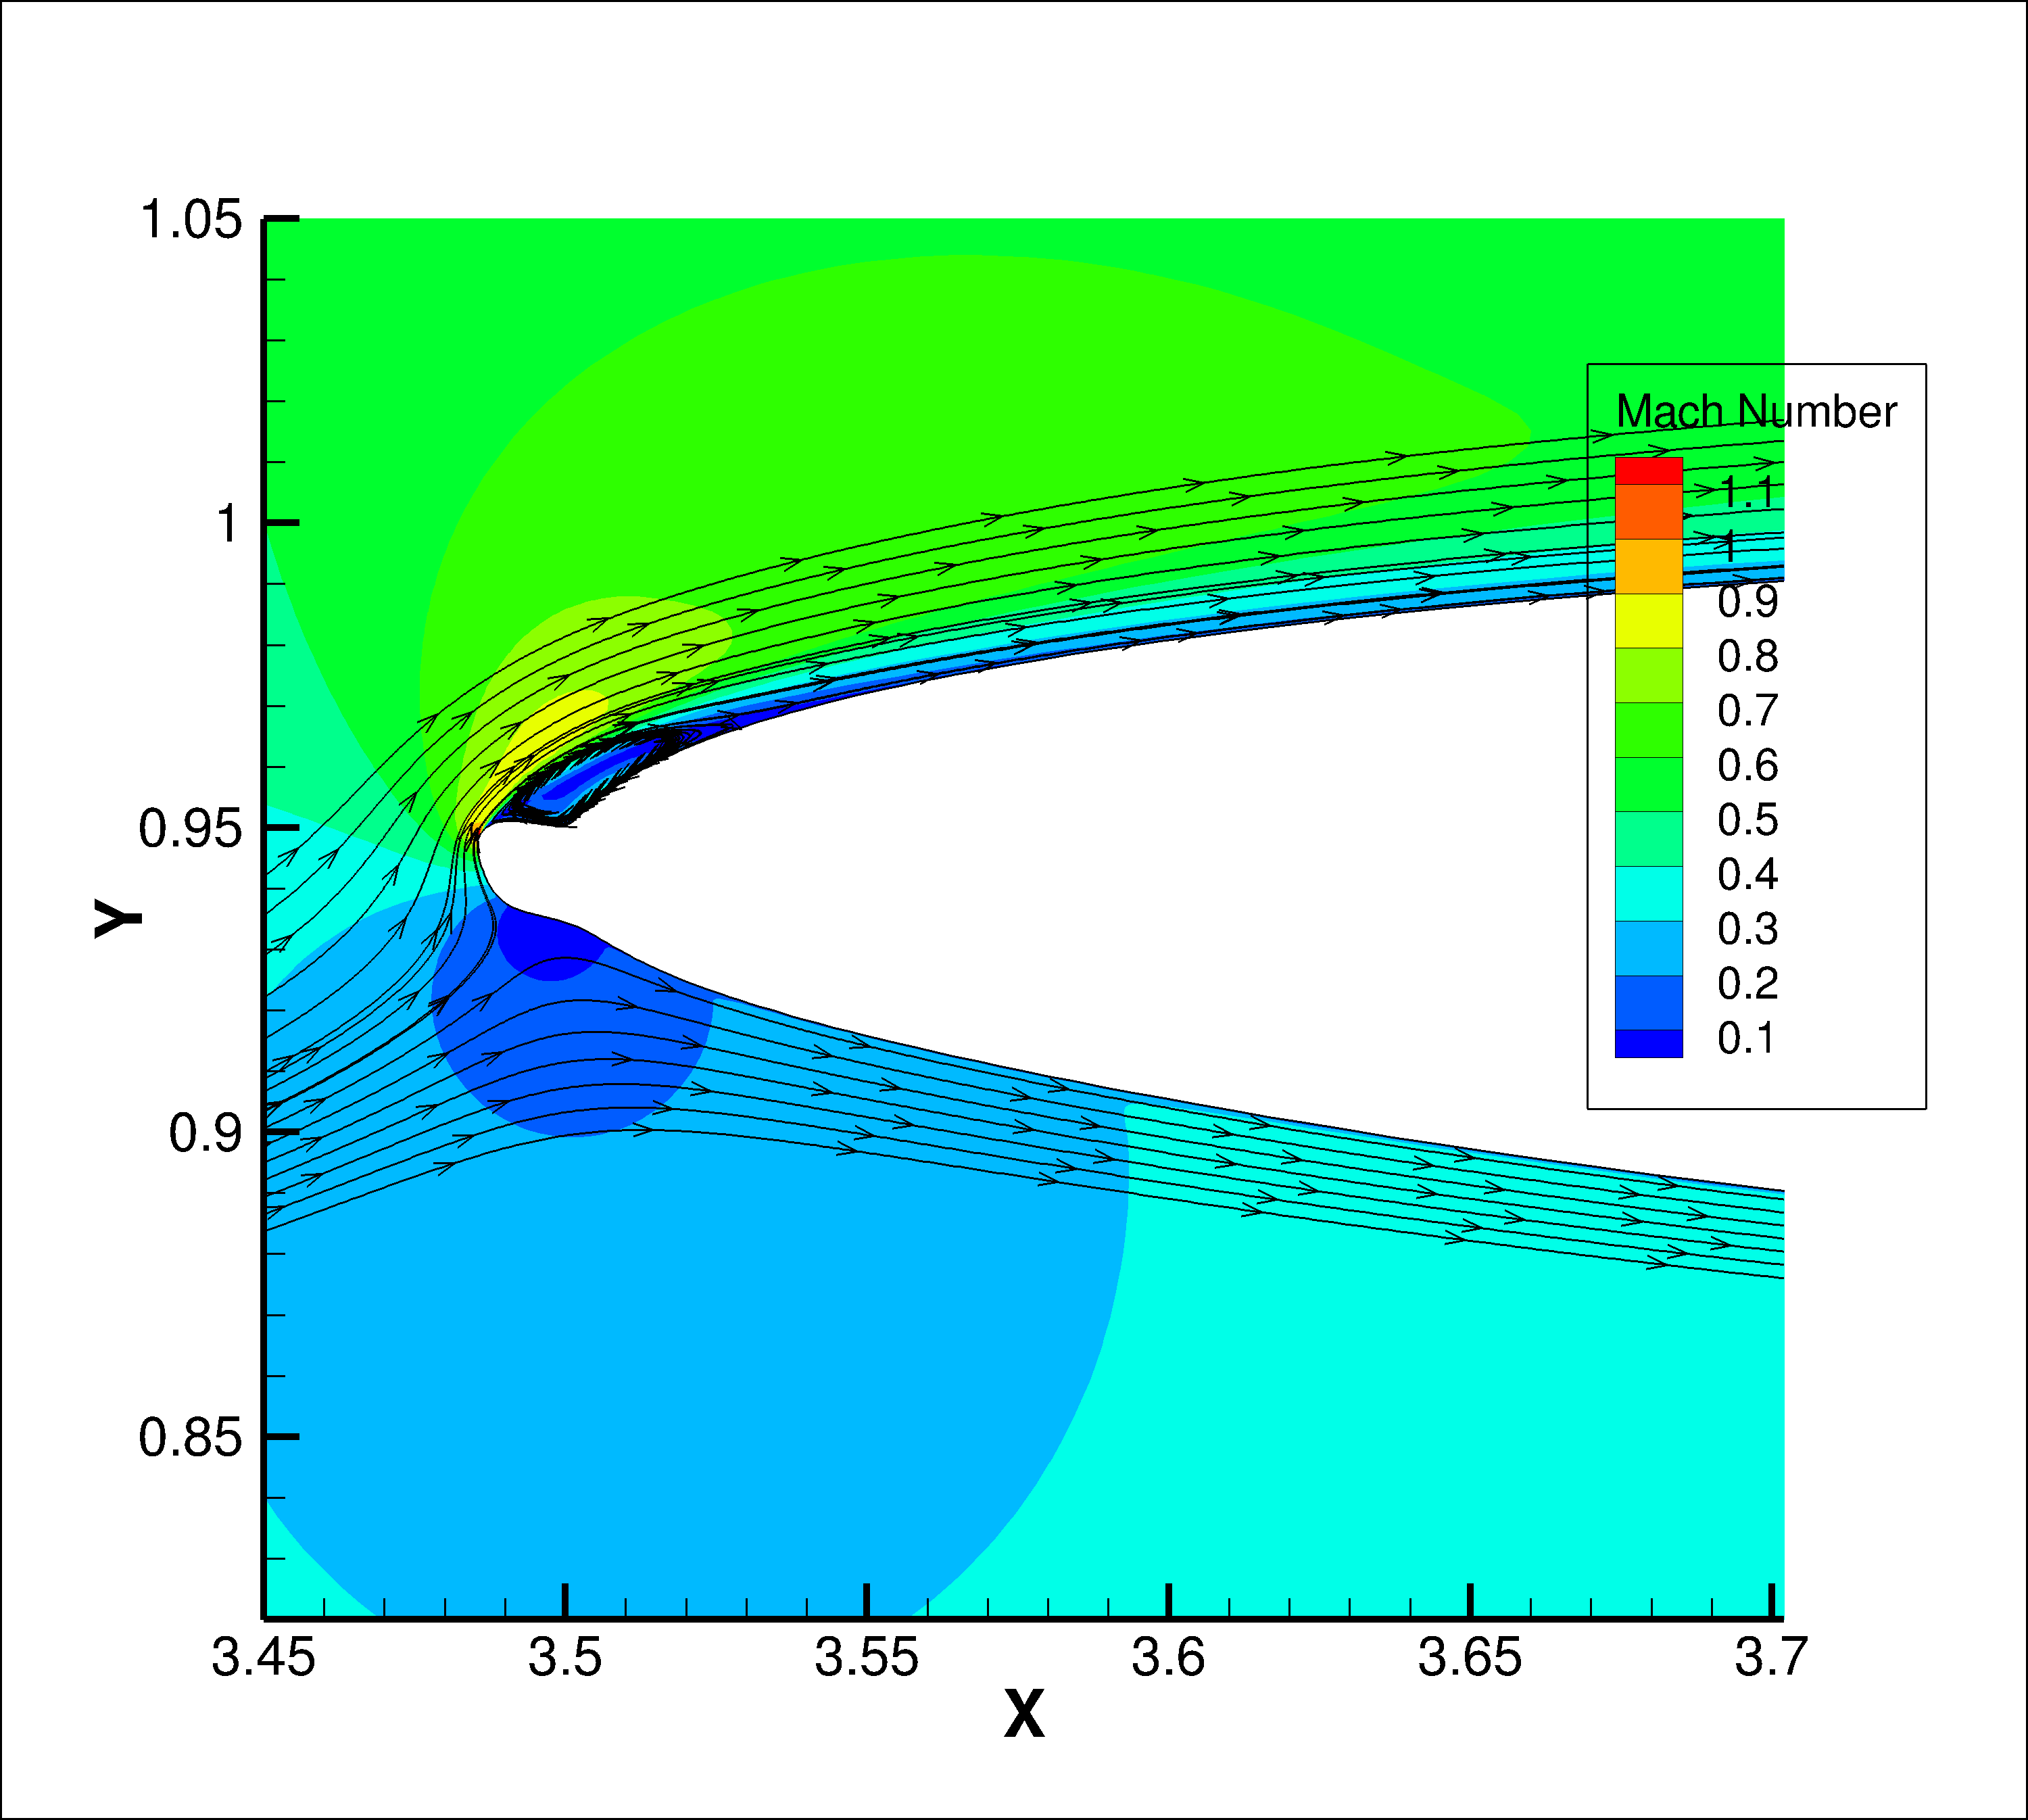
\includegraphics[width=1\textwidth]{GoodHorn.png} \\
    {\bf Favorable Position}
    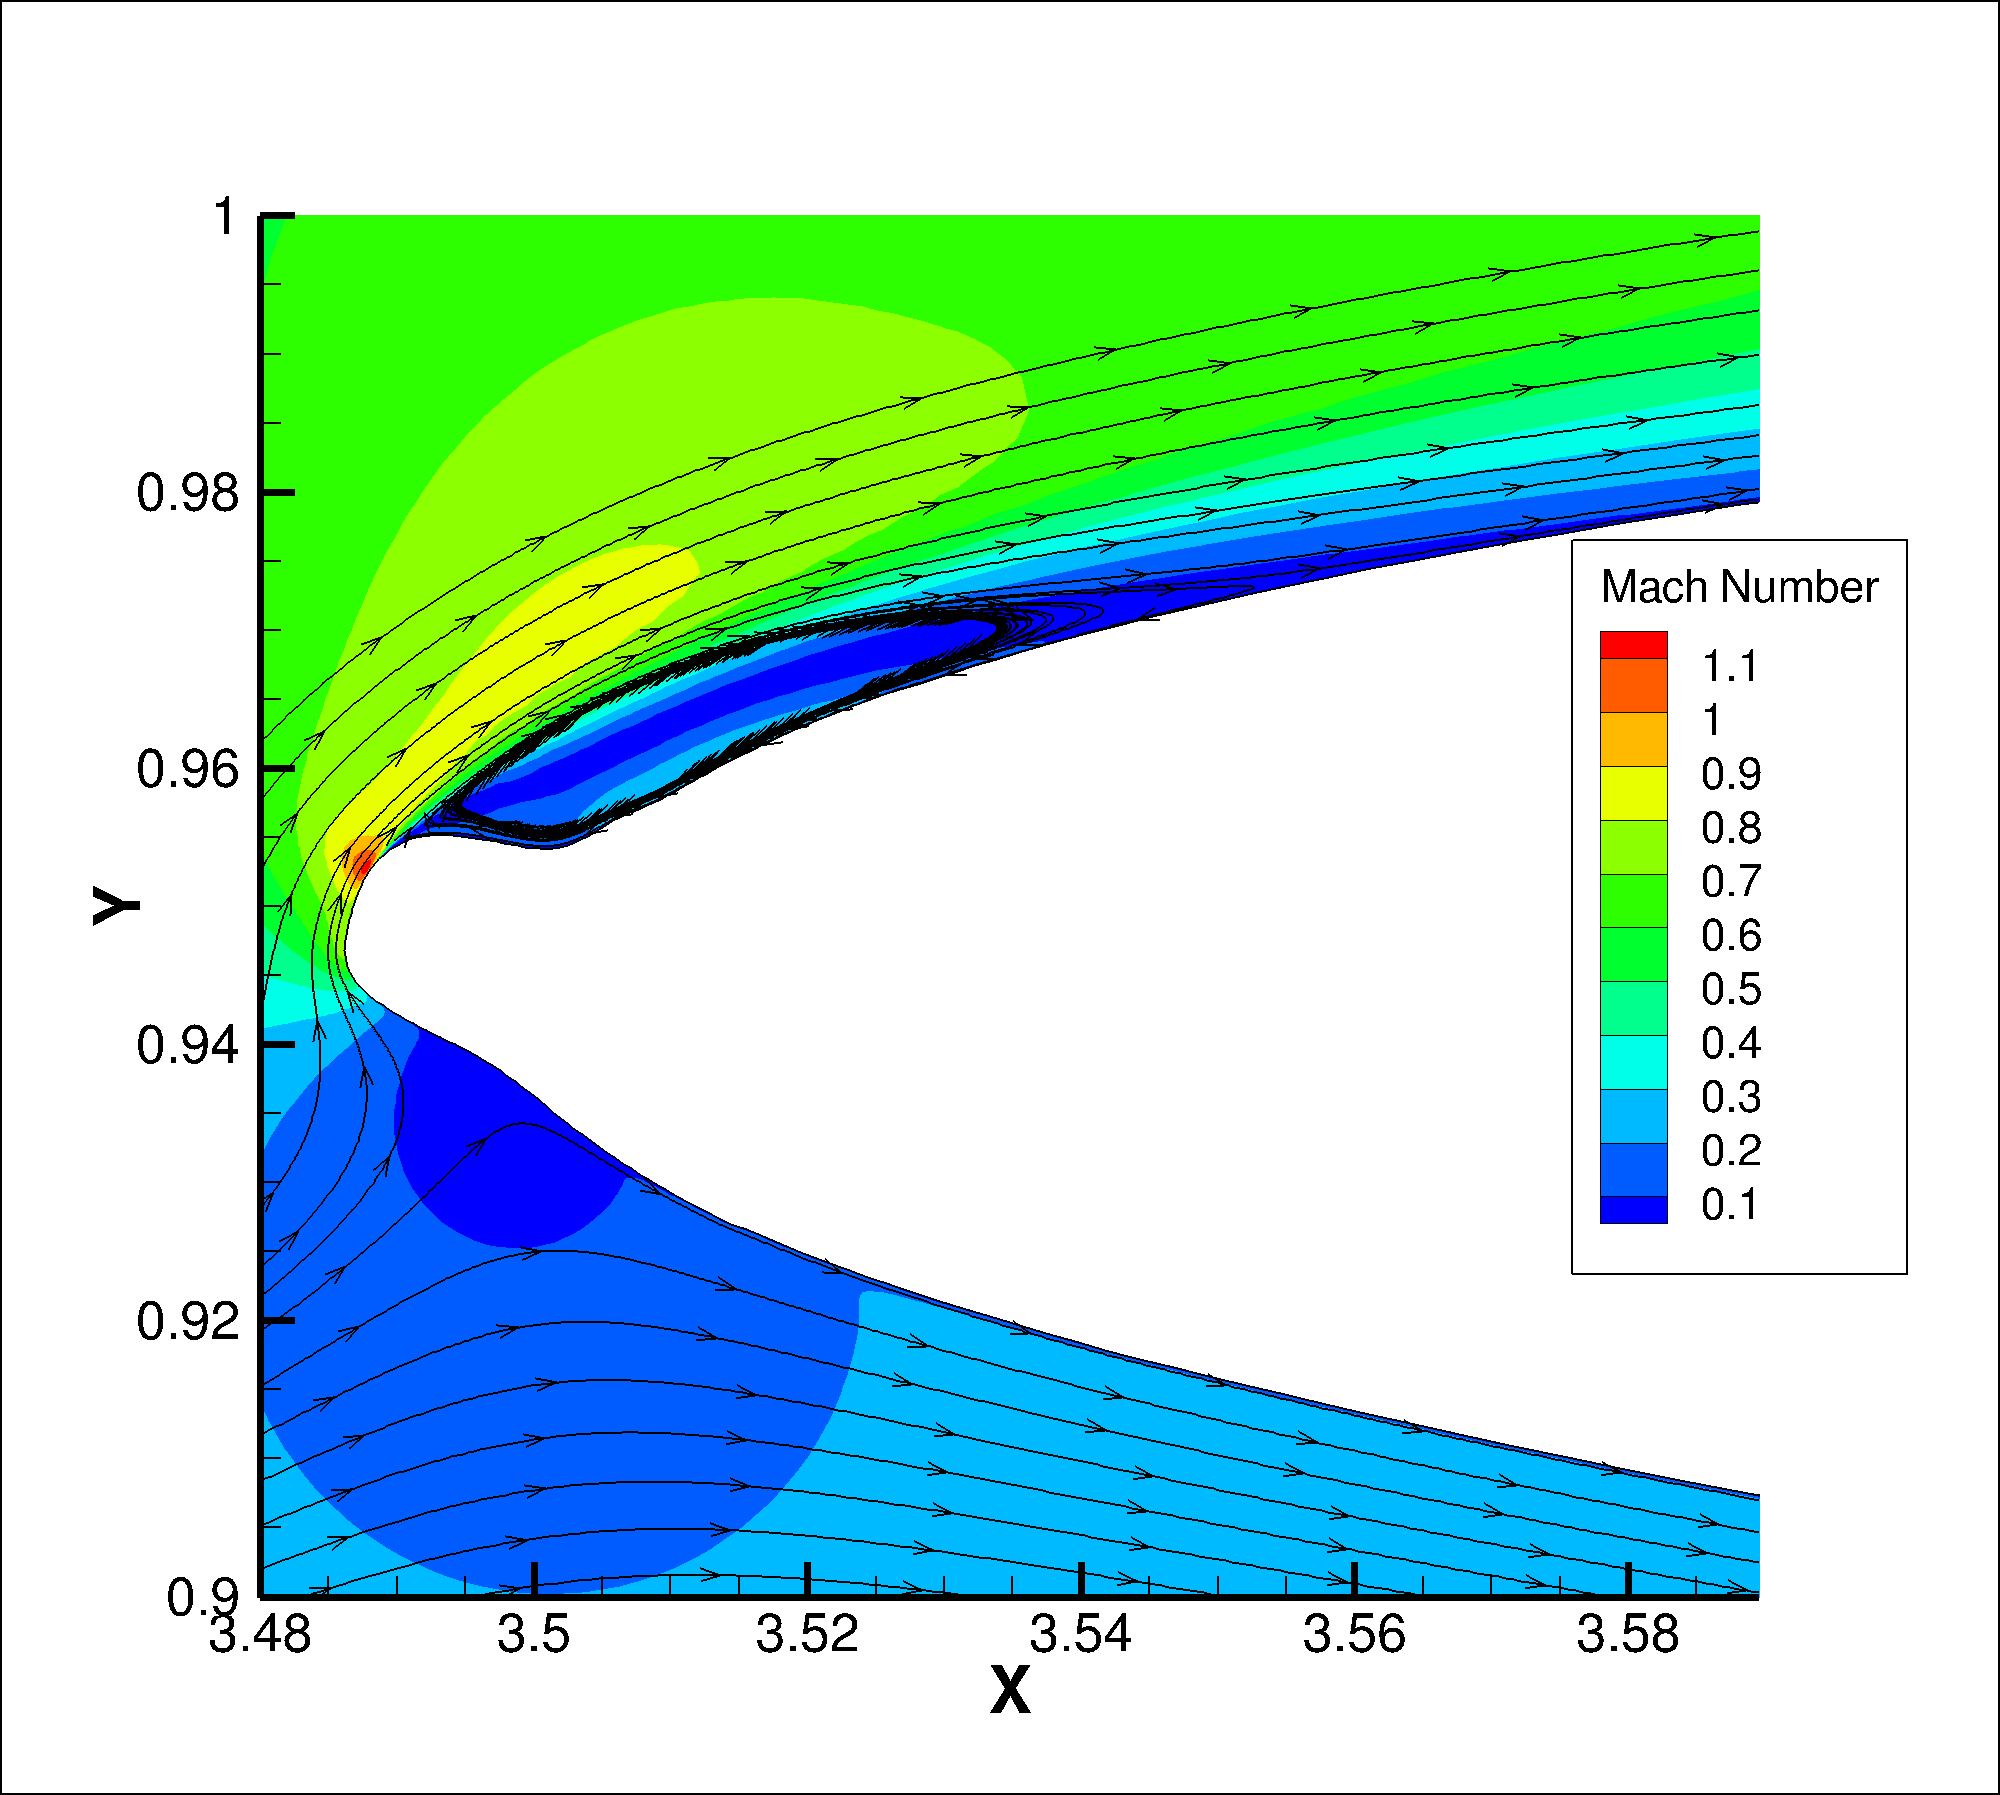
\includegraphics[width=1\textwidth]{GoodHornPOD.png} \\
    {\bf Favorable shape skew}
  \column{0.30\textwidth}
    \centering
    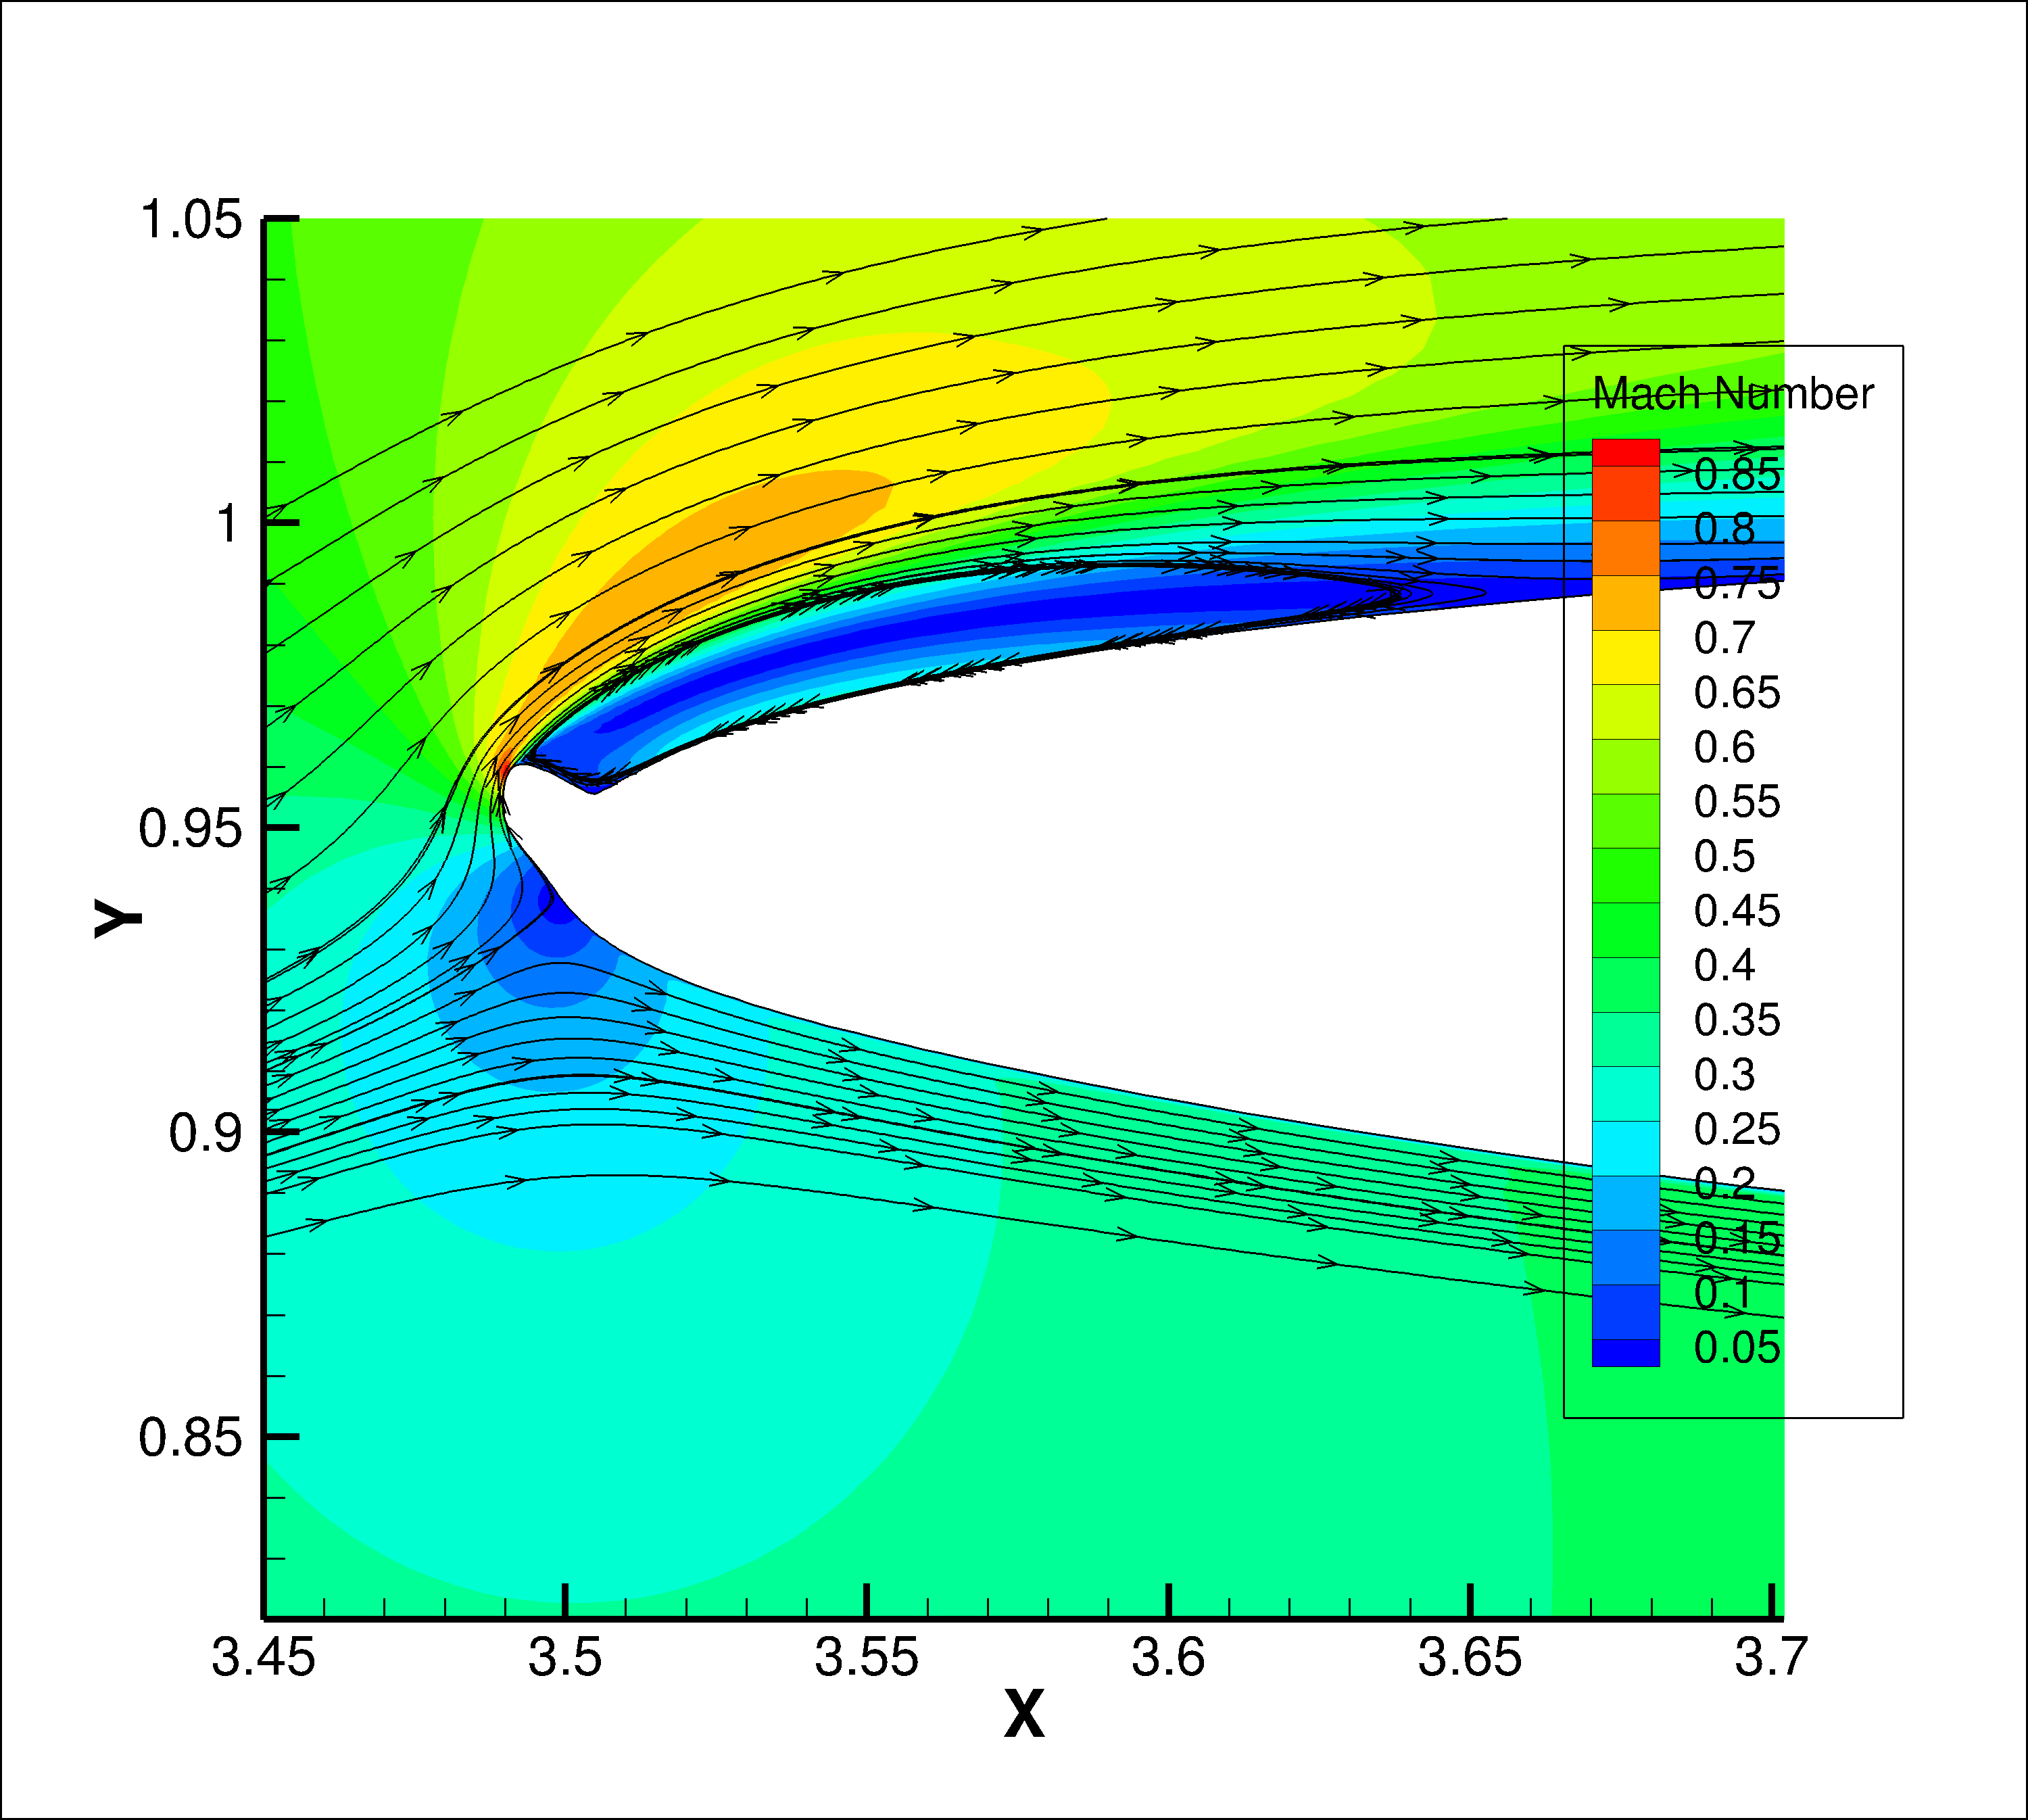
\includegraphics[width=1\textwidth]{BadHorn.png} \\
    {\bf Unfavorable Position}
    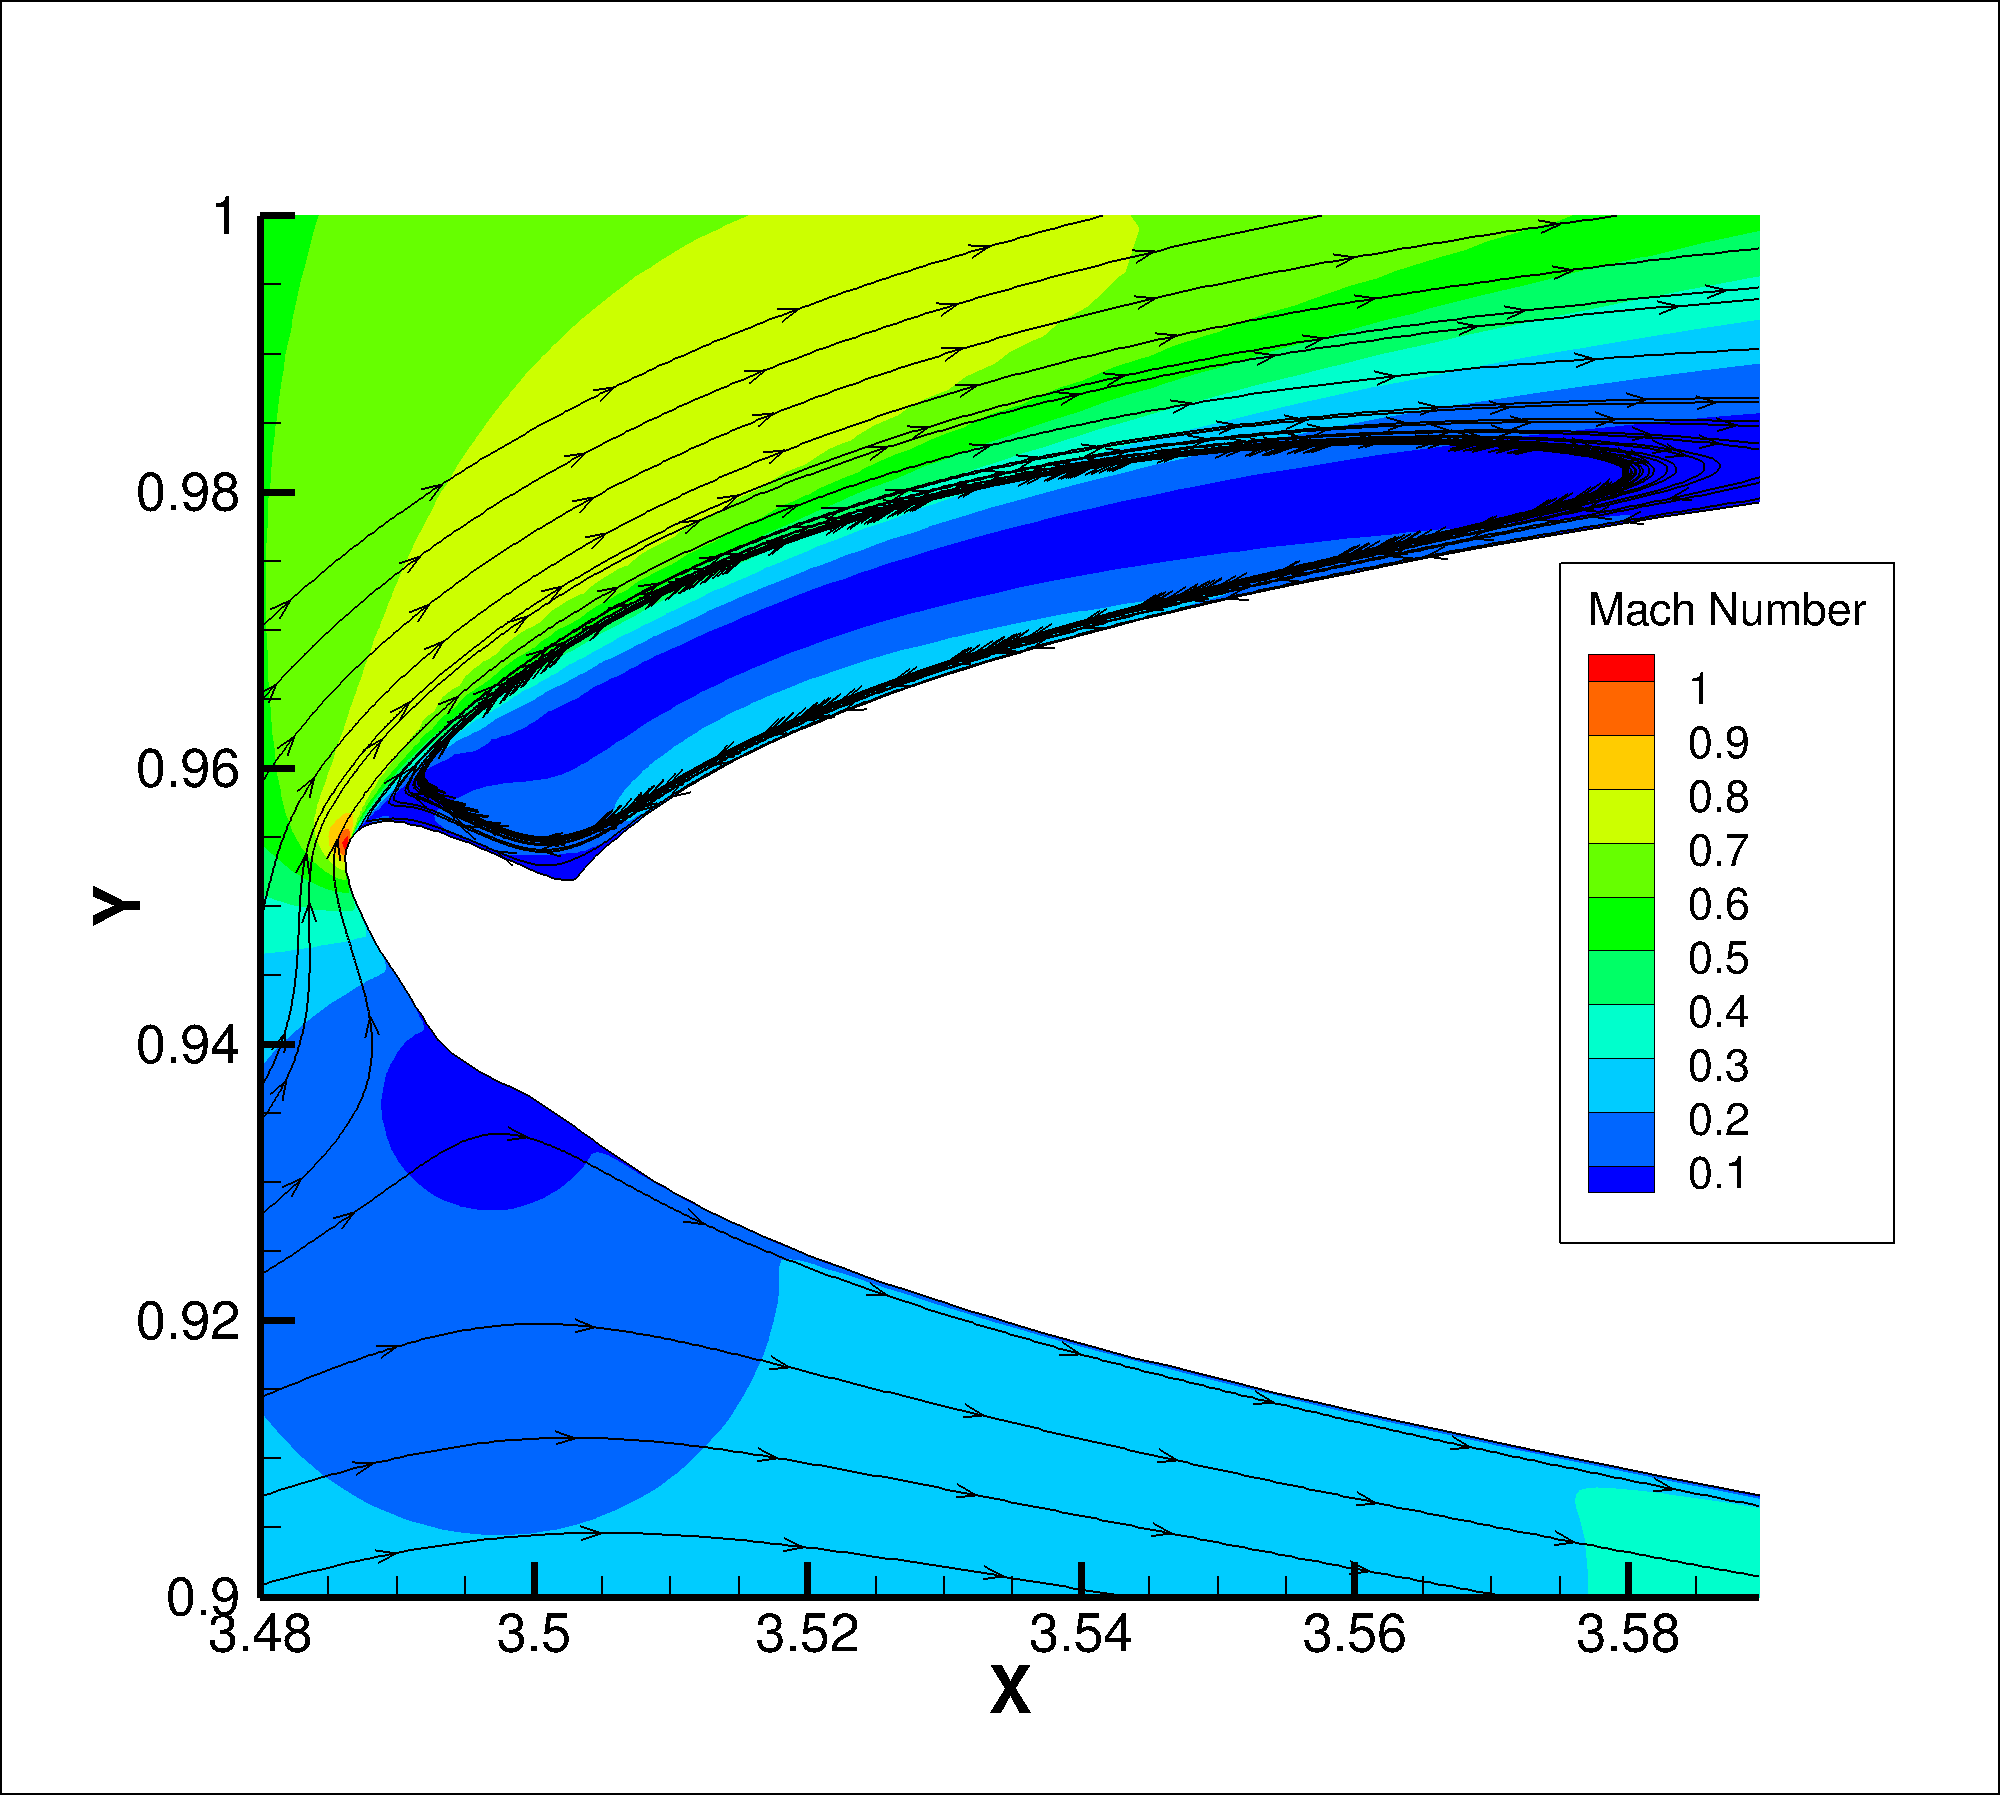
\includegraphics[width=1\textwidth]{BadHornPOD.png} \\
    {\bf Unfavorable shape skew}
\end{columns}
\end{frame}
\section{Experiment Dataset}
\label{sec-4}
\begin{frame}
\frametitle{Dataset Description}
\label{sec-4-1}


\begin{figure}
  \centering
  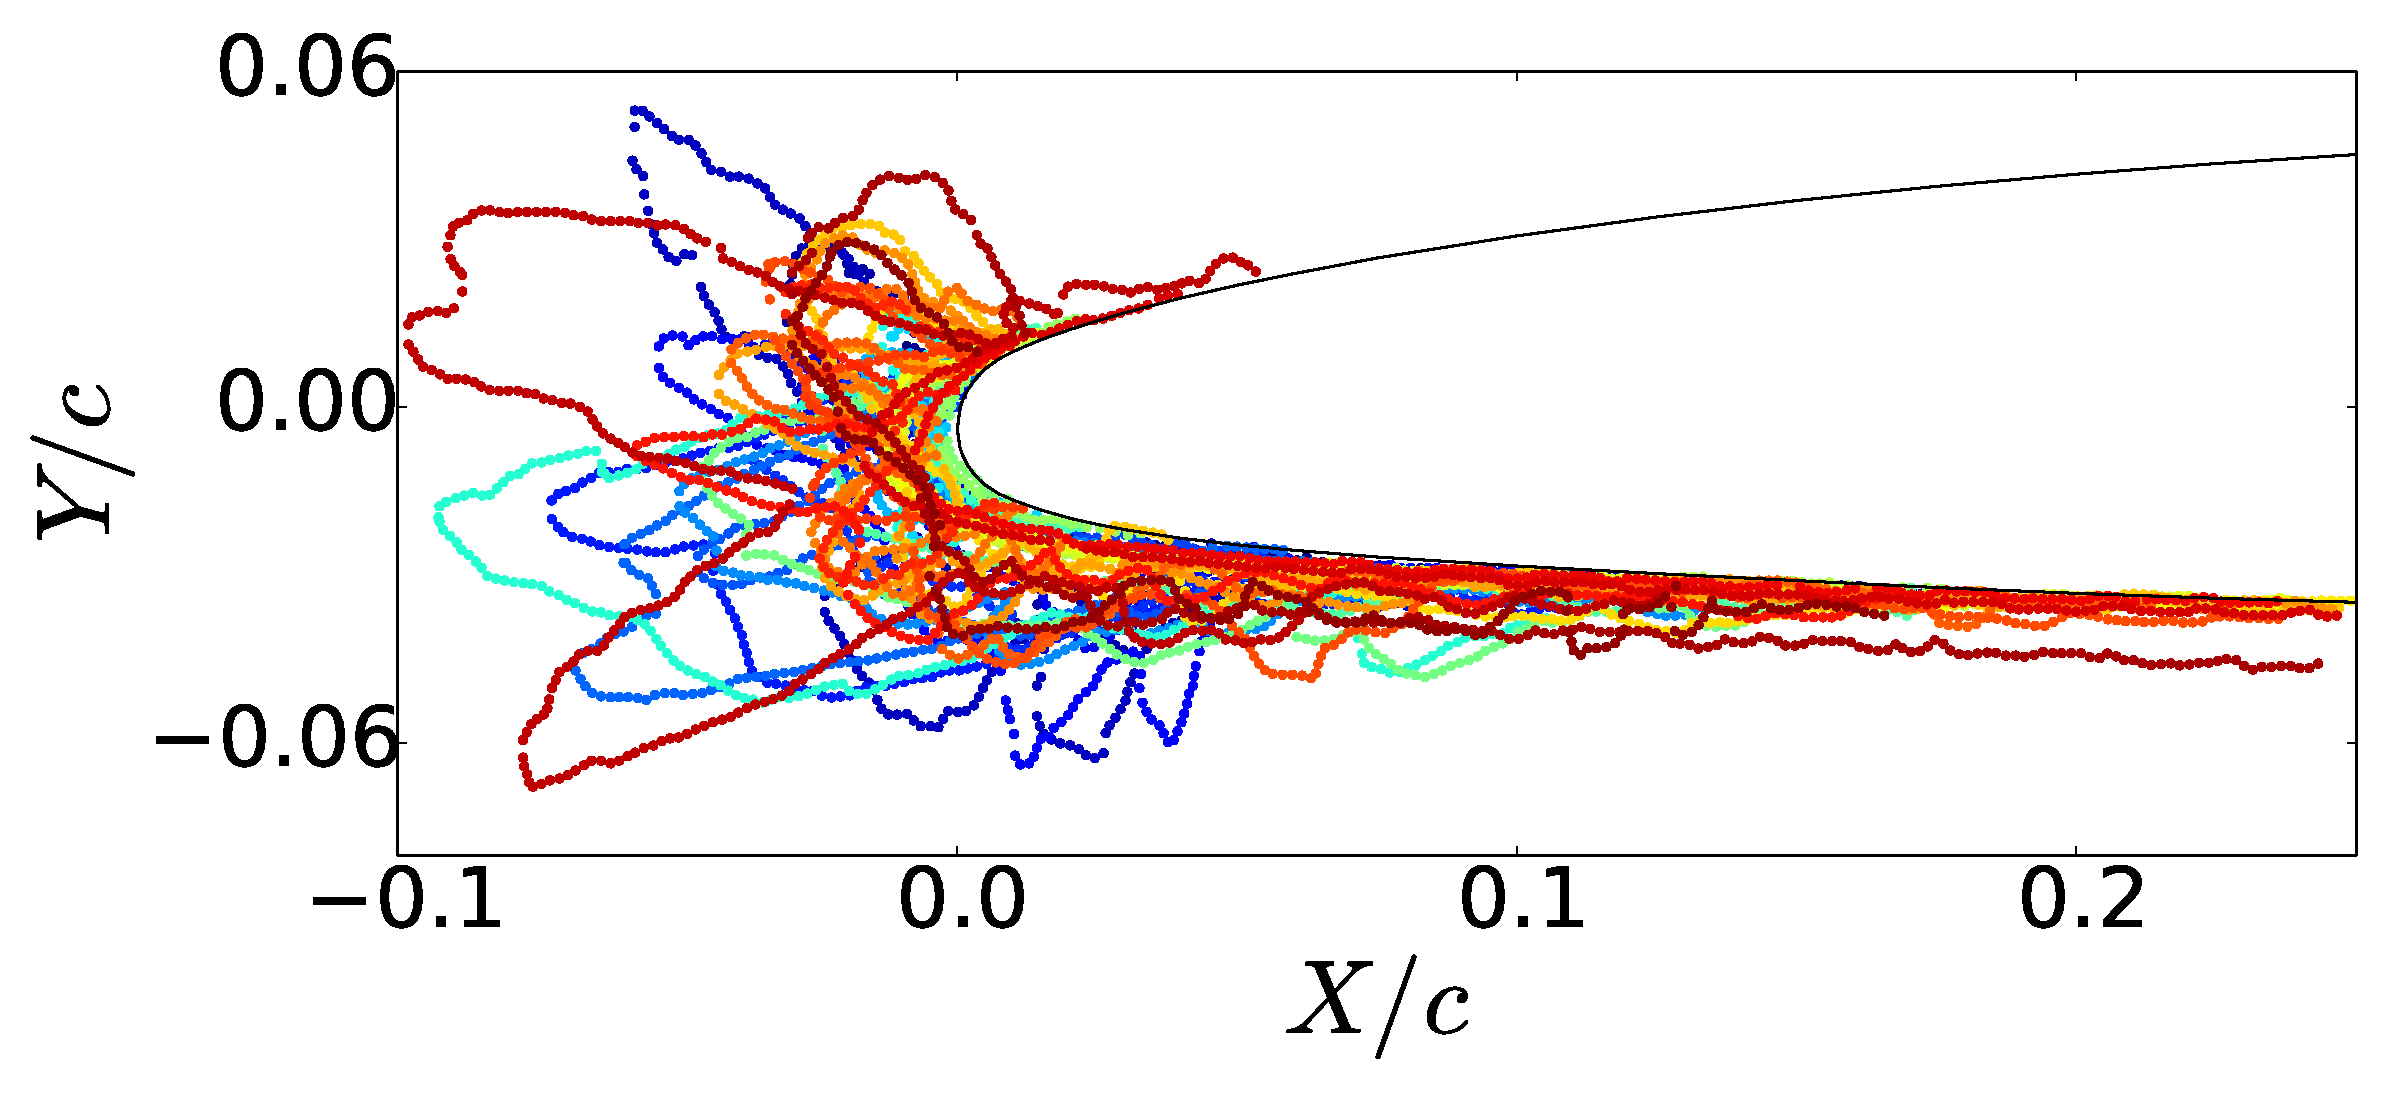
\includegraphics[width=0.7\textwidth]{Dataset}
\end{figure}

\begin{itemize}
\item Business jet clean airfoil geometry\footnote{Addy, H.E. \emph{Ice Accretions and Icing Effects for Modern Airfoils}. NASA TR 2000-210031.
 }
\item 54 ice shapes, exposed to wide range of various icing conditions
  consistent with FAA certification guidelines
\item POD dataset will consist of binary values defined on a static
  Cartesian mesh (`1' if mesh point is on the ice, `0' if not)
\end{itemize}
\end{frame}
\begin{frame}
\frametitle{Low-Dimensional Modeling of Dataset}
\label{sec-4-2}


\begin{columns}[c]
  \column{0.45\textwidth}
    \centering
    \hspace{-2.17em}
    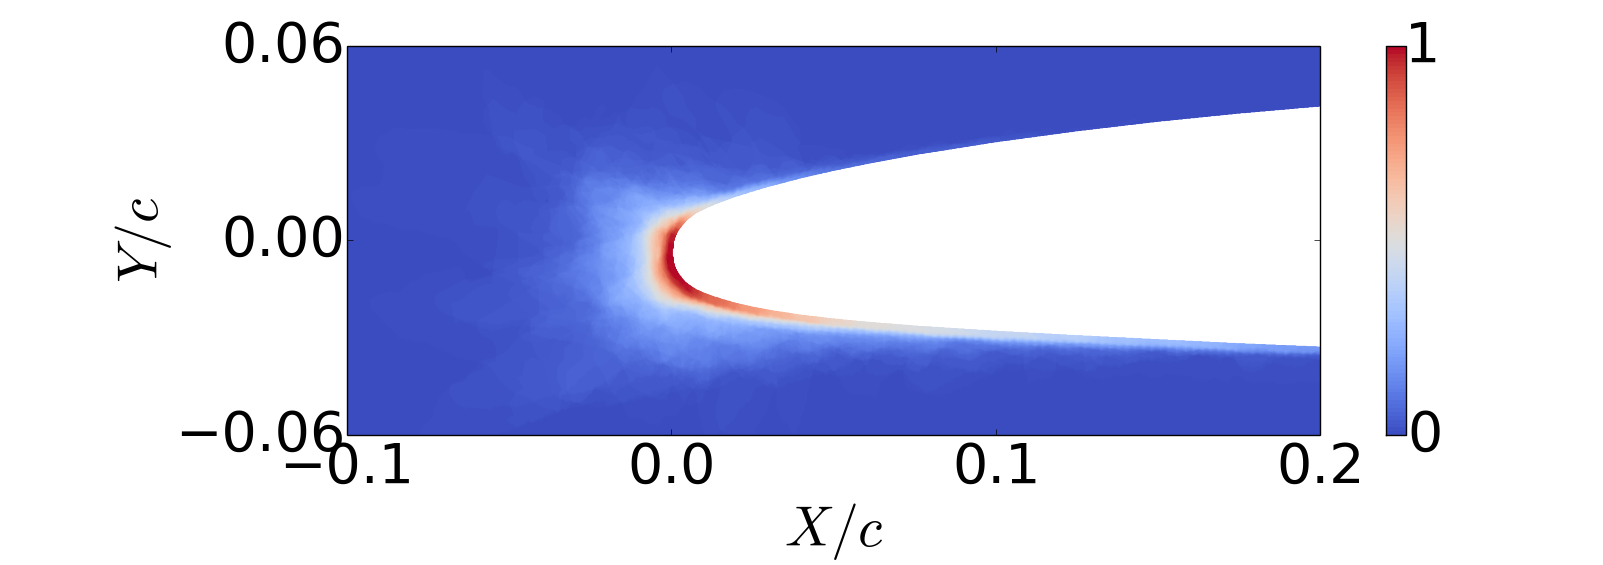
\includegraphics[width=0.9\textwidth]{MEAN.png} \\
    {\bf Mean} \\
    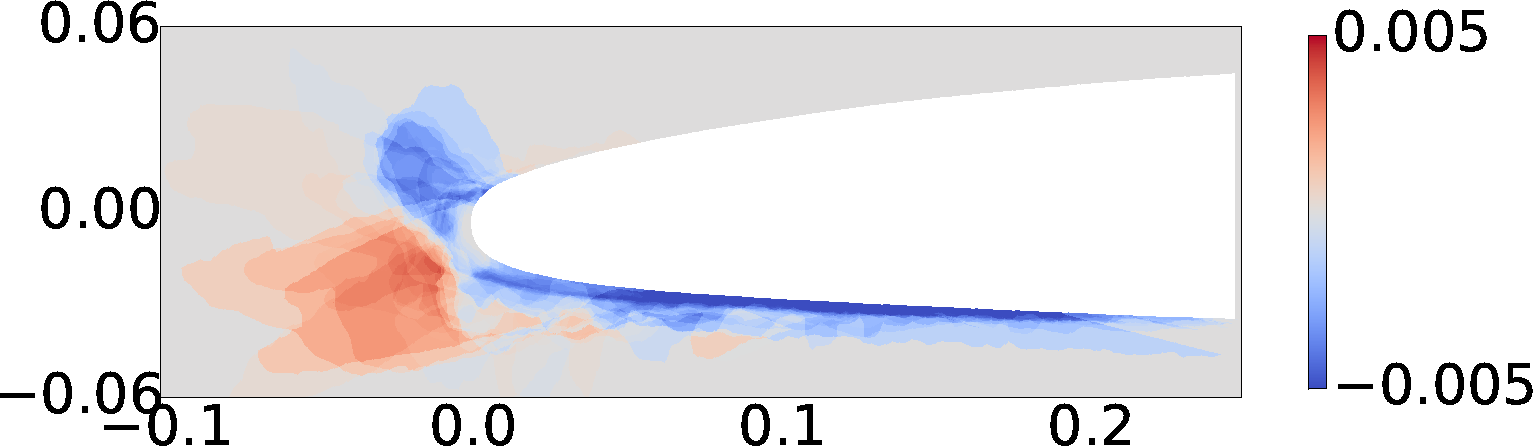
\includegraphics[width=1\textwidth]{MODE2.png} \\
    {\bf Mode 2} \\
    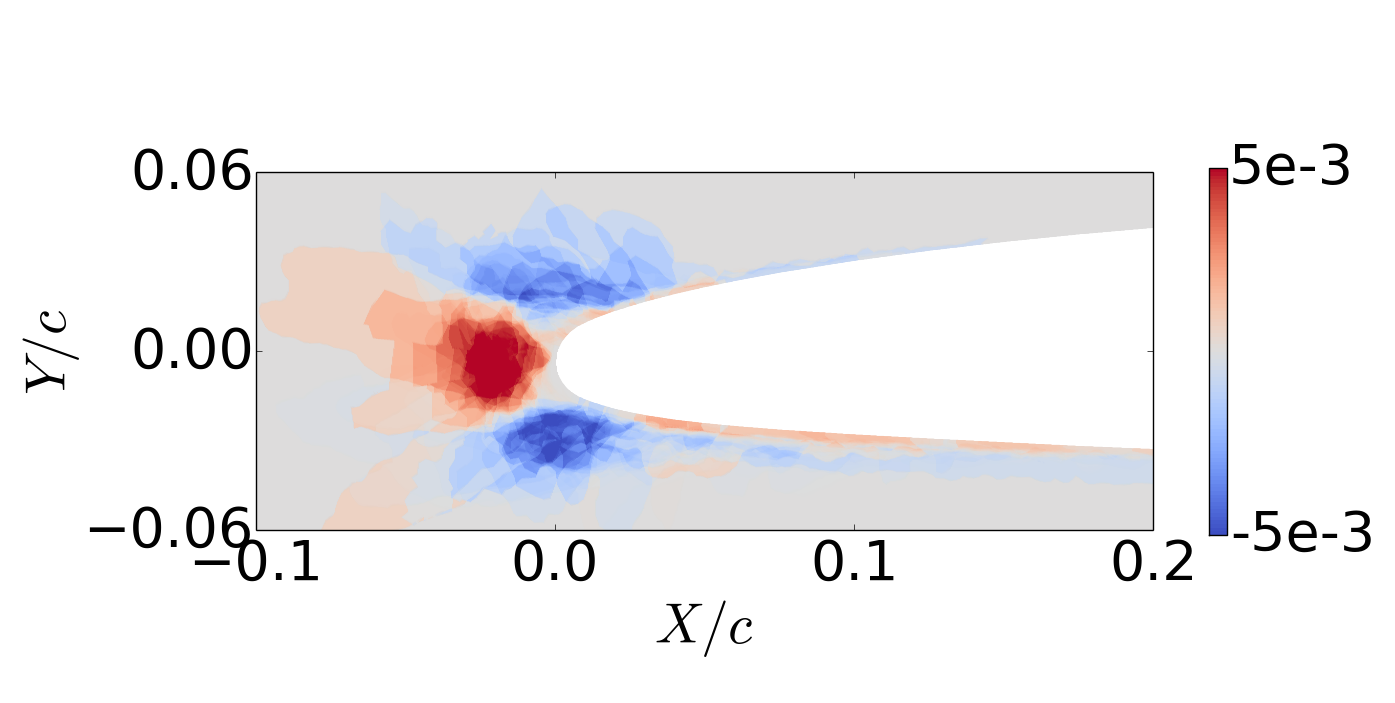
\includegraphics[width=1\textwidth]{MODE4.png} \\
    {\bf Mode 4}
  \column{0.45\textwidth}
    \centering
    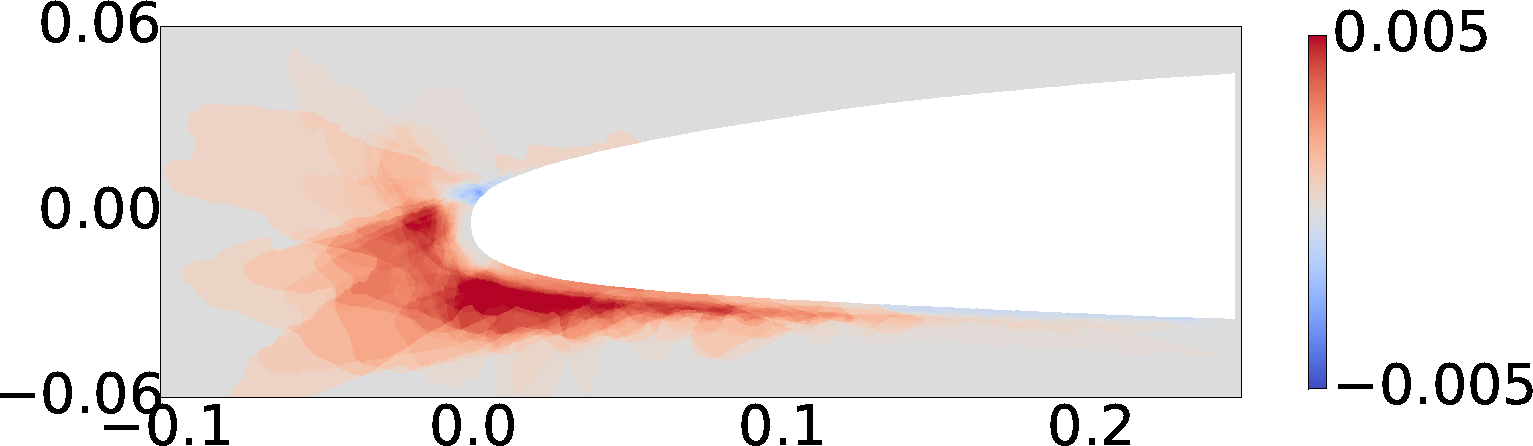
\includegraphics[width=1\textwidth]{MODE1.png} \\
    {\bf Mode 1} \\
    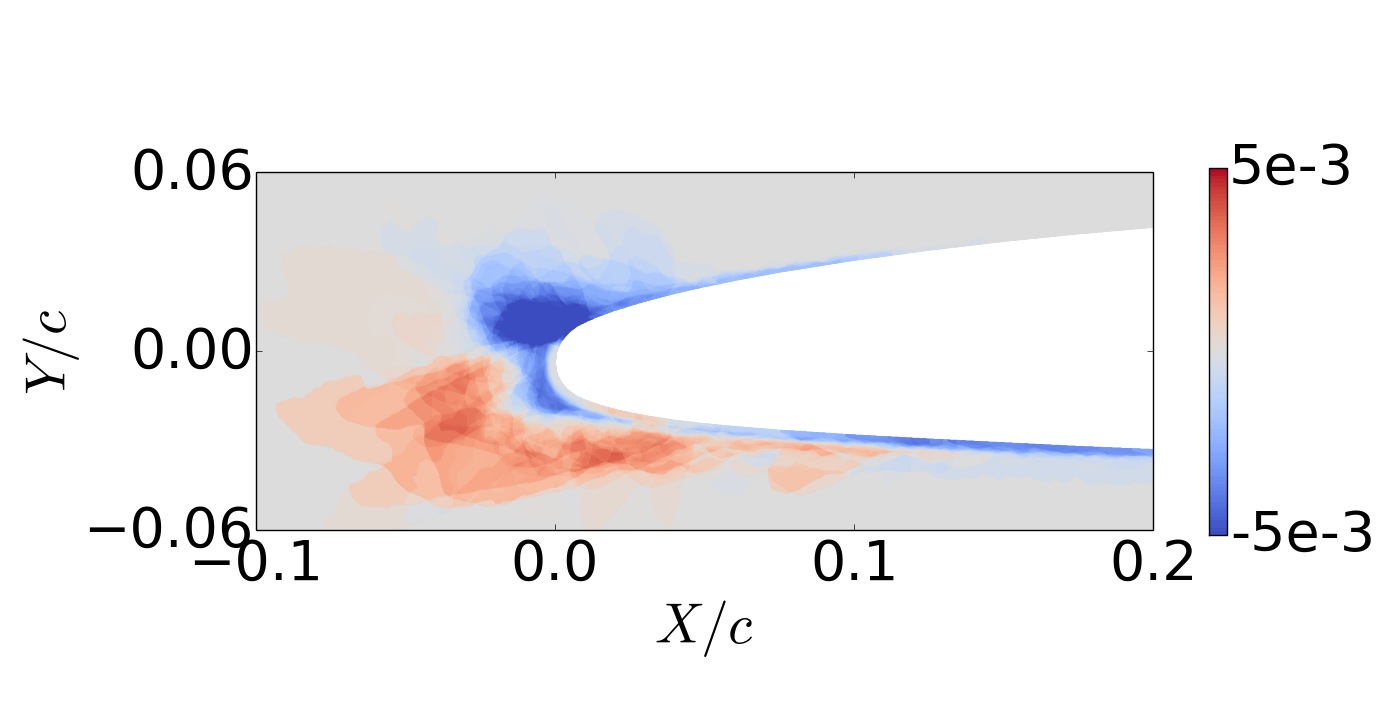
\includegraphics[width=1\textwidth]{MODE3.png} \\
    {\bf Mode 3} \\
    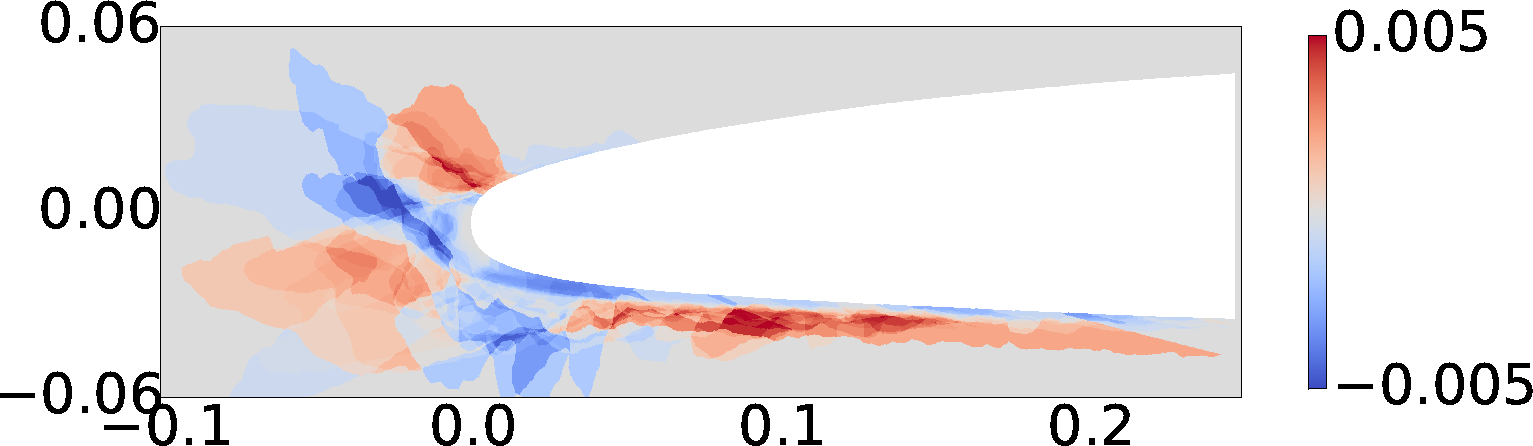
\includegraphics[width=1\textwidth]{MODE5.png} \\
    {\bf Mode 5}
\end{columns}


\begin{itemize}
\item 8 Modes retained; this is where POD eigenvalue magnitudes have
  decayed by an order of magnitude
\end{itemize}
\end{frame}
\begin{frame}
\frametitle{Ice Shape Reconstructions}
\label{sec-4-3}


\begin{columns}[c]
  \column{0.45\textwidth}
    \centering
    \hspace{-0.5em}
    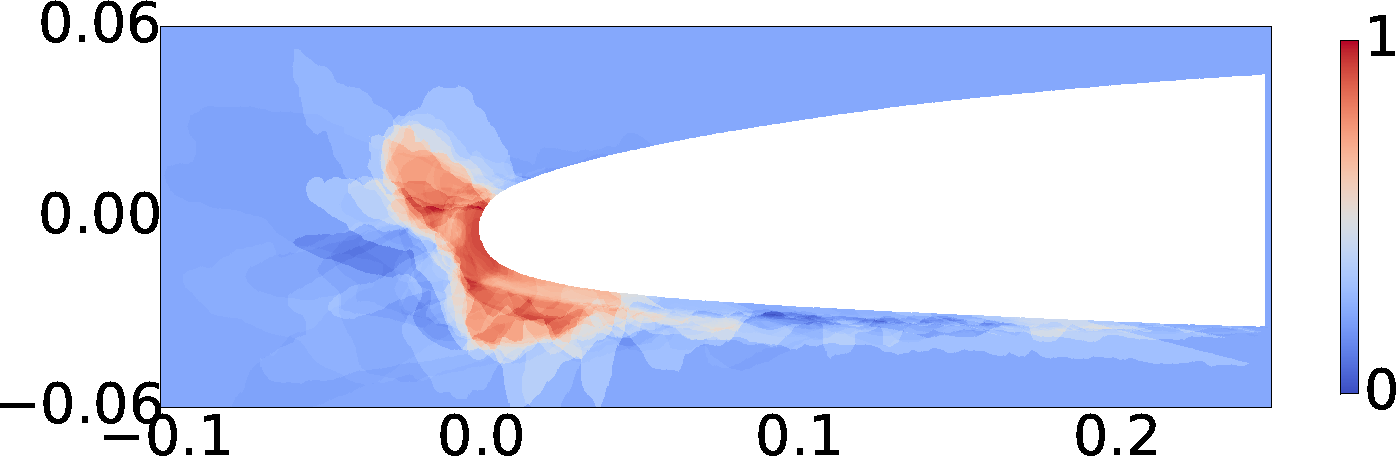
\includegraphics[width=1\textwidth]{UnfilteredReconstruction.png} \\
    {\bf Unfiltered Reconstruction} \\
    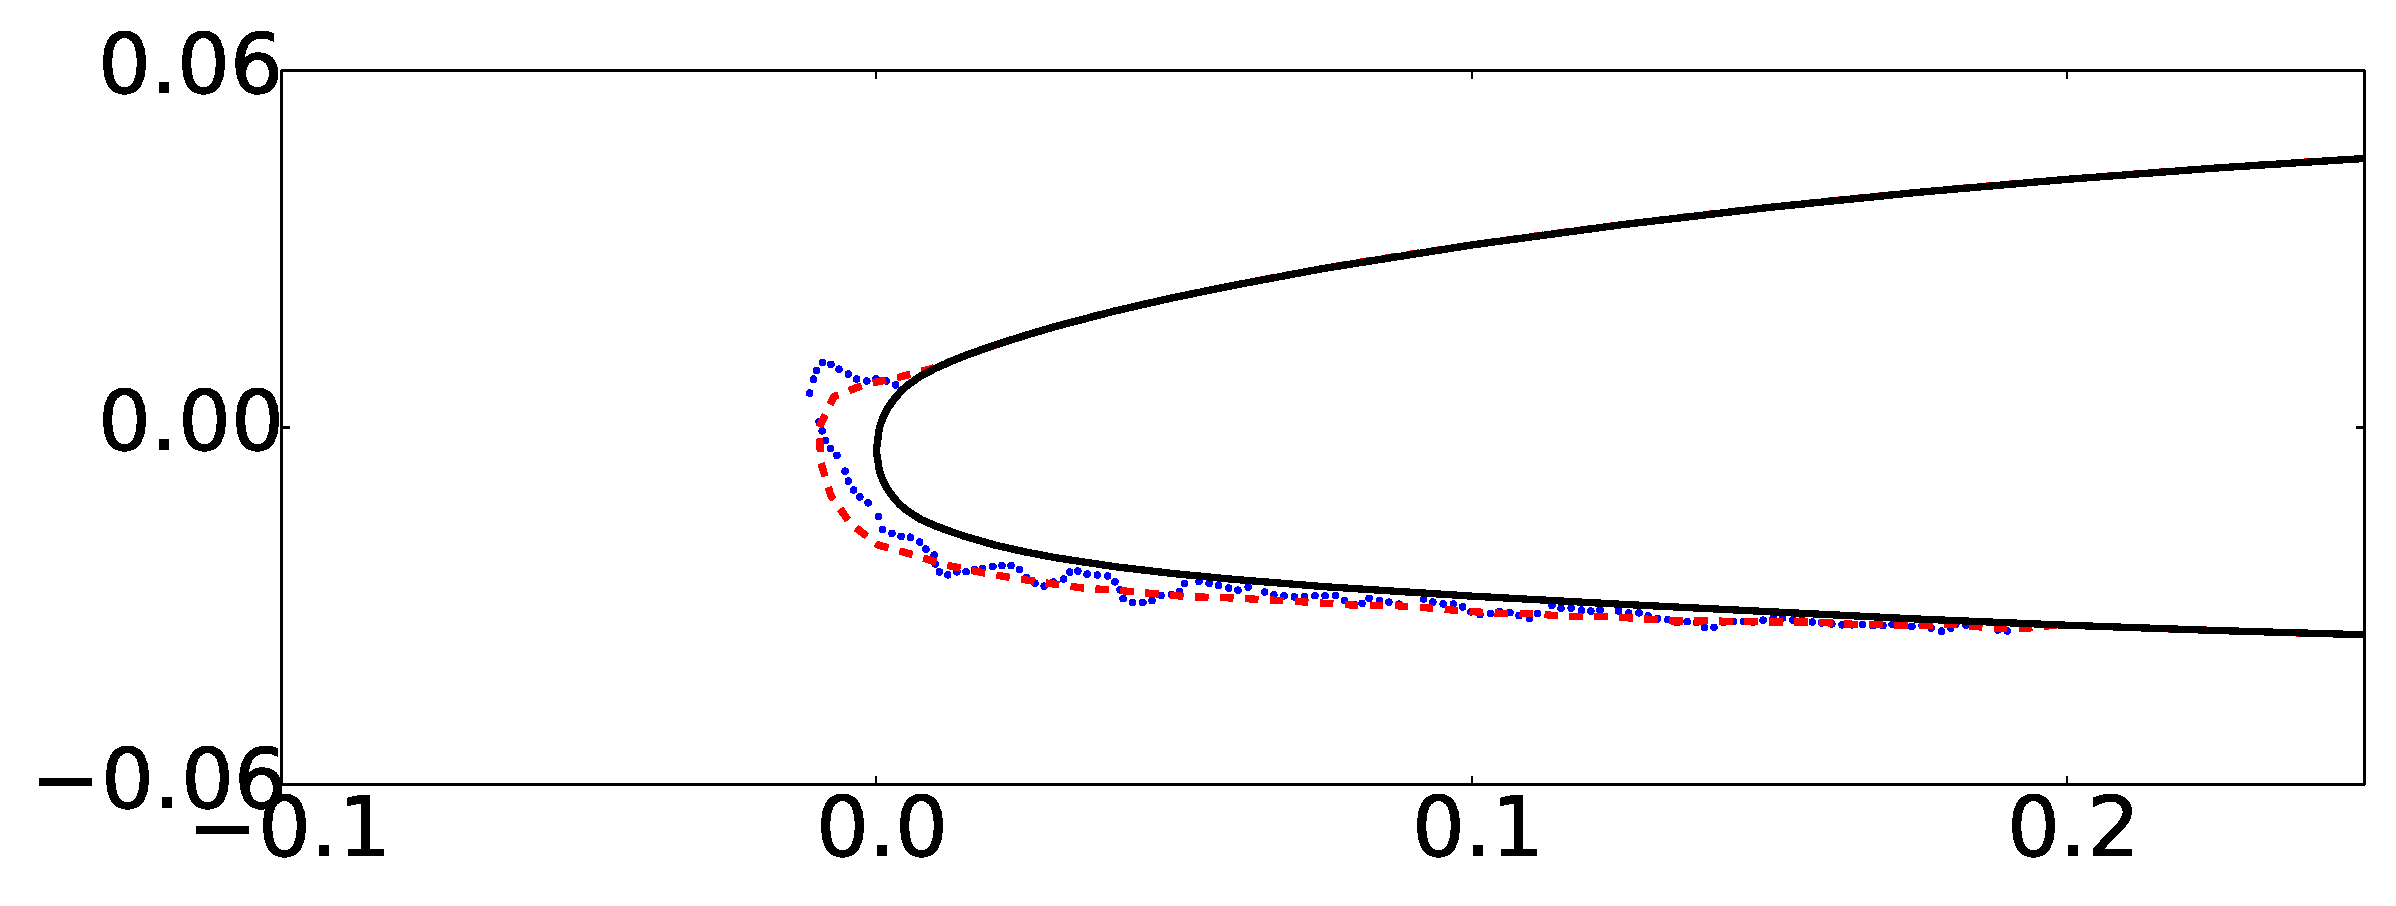
\includegraphics[width=1\textwidth]{ReconstructionE1} \\
    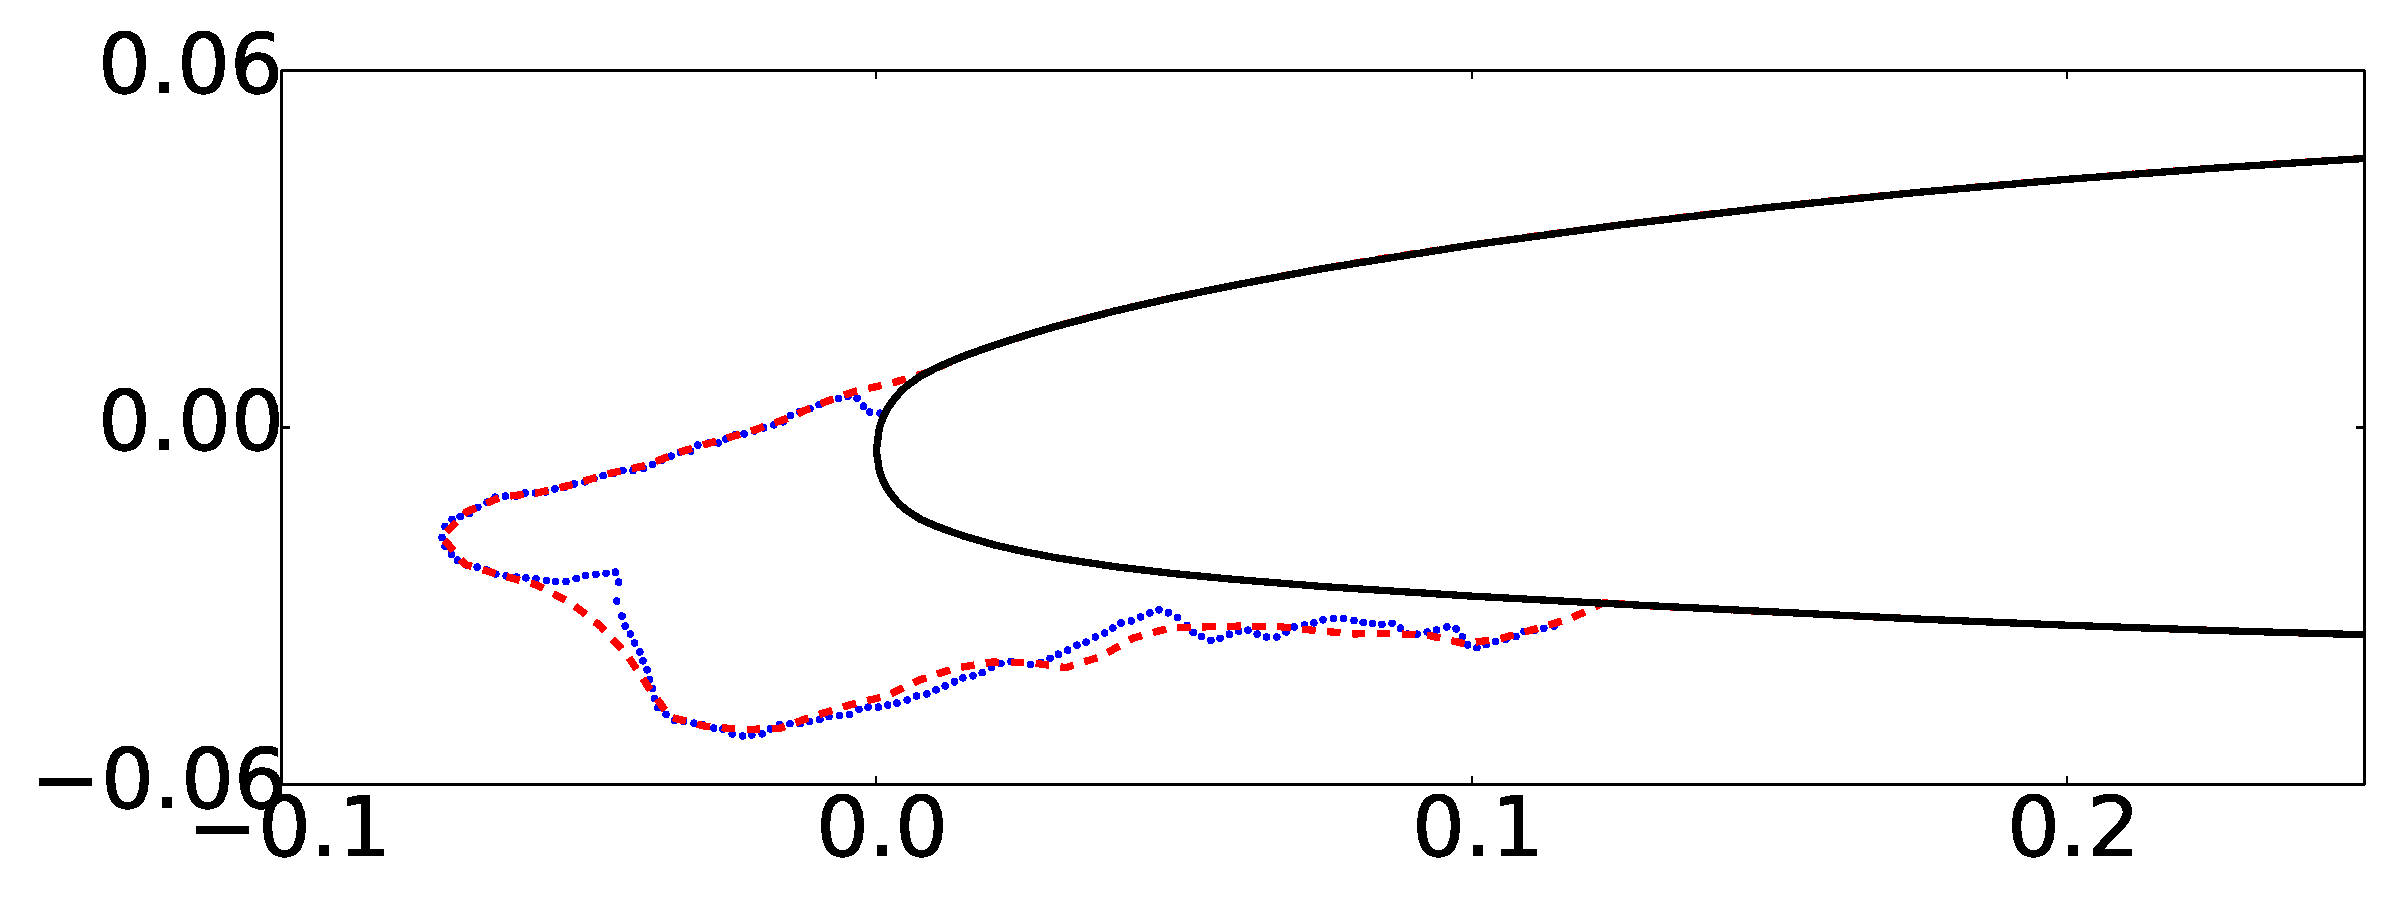
\includegraphics[width=1\textwidth]{ReconstructionE9} \\
  \column{0.45\textwidth}
    \centering
    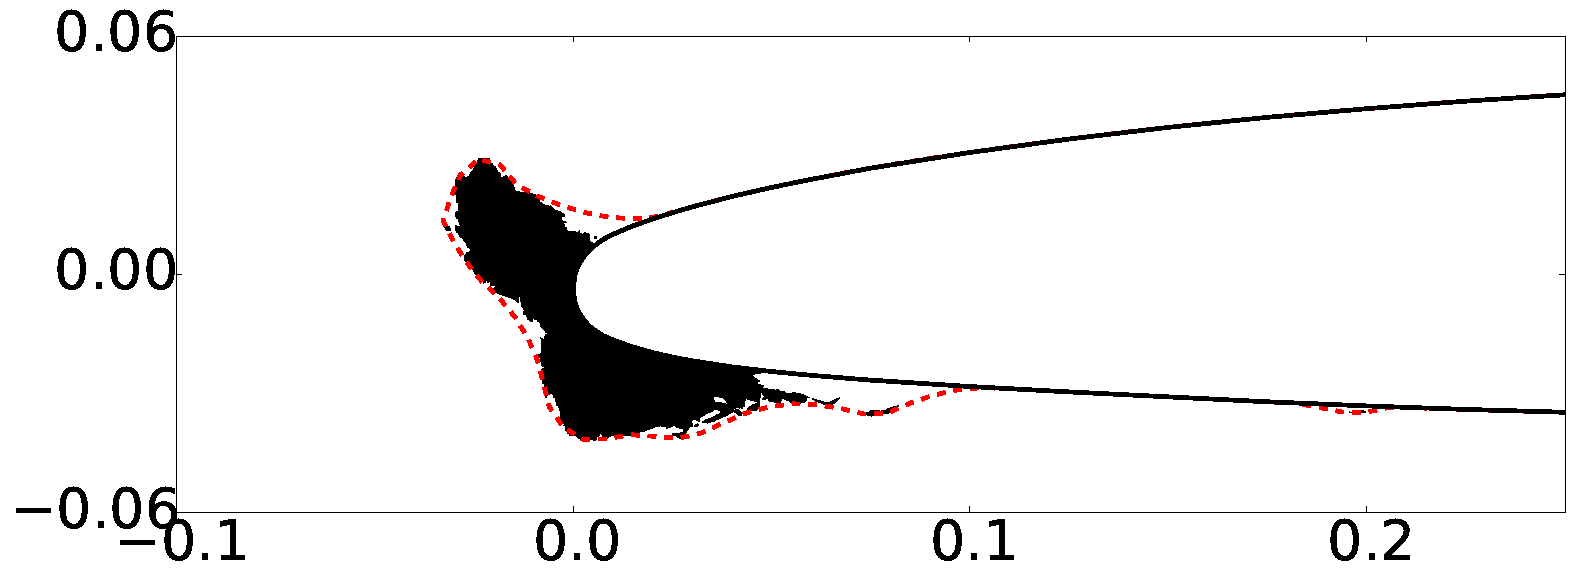
\includegraphics[width=1\textwidth]{FilteredReconstruction.png} \\
    {\bf Filtered Reconstruction} \\
    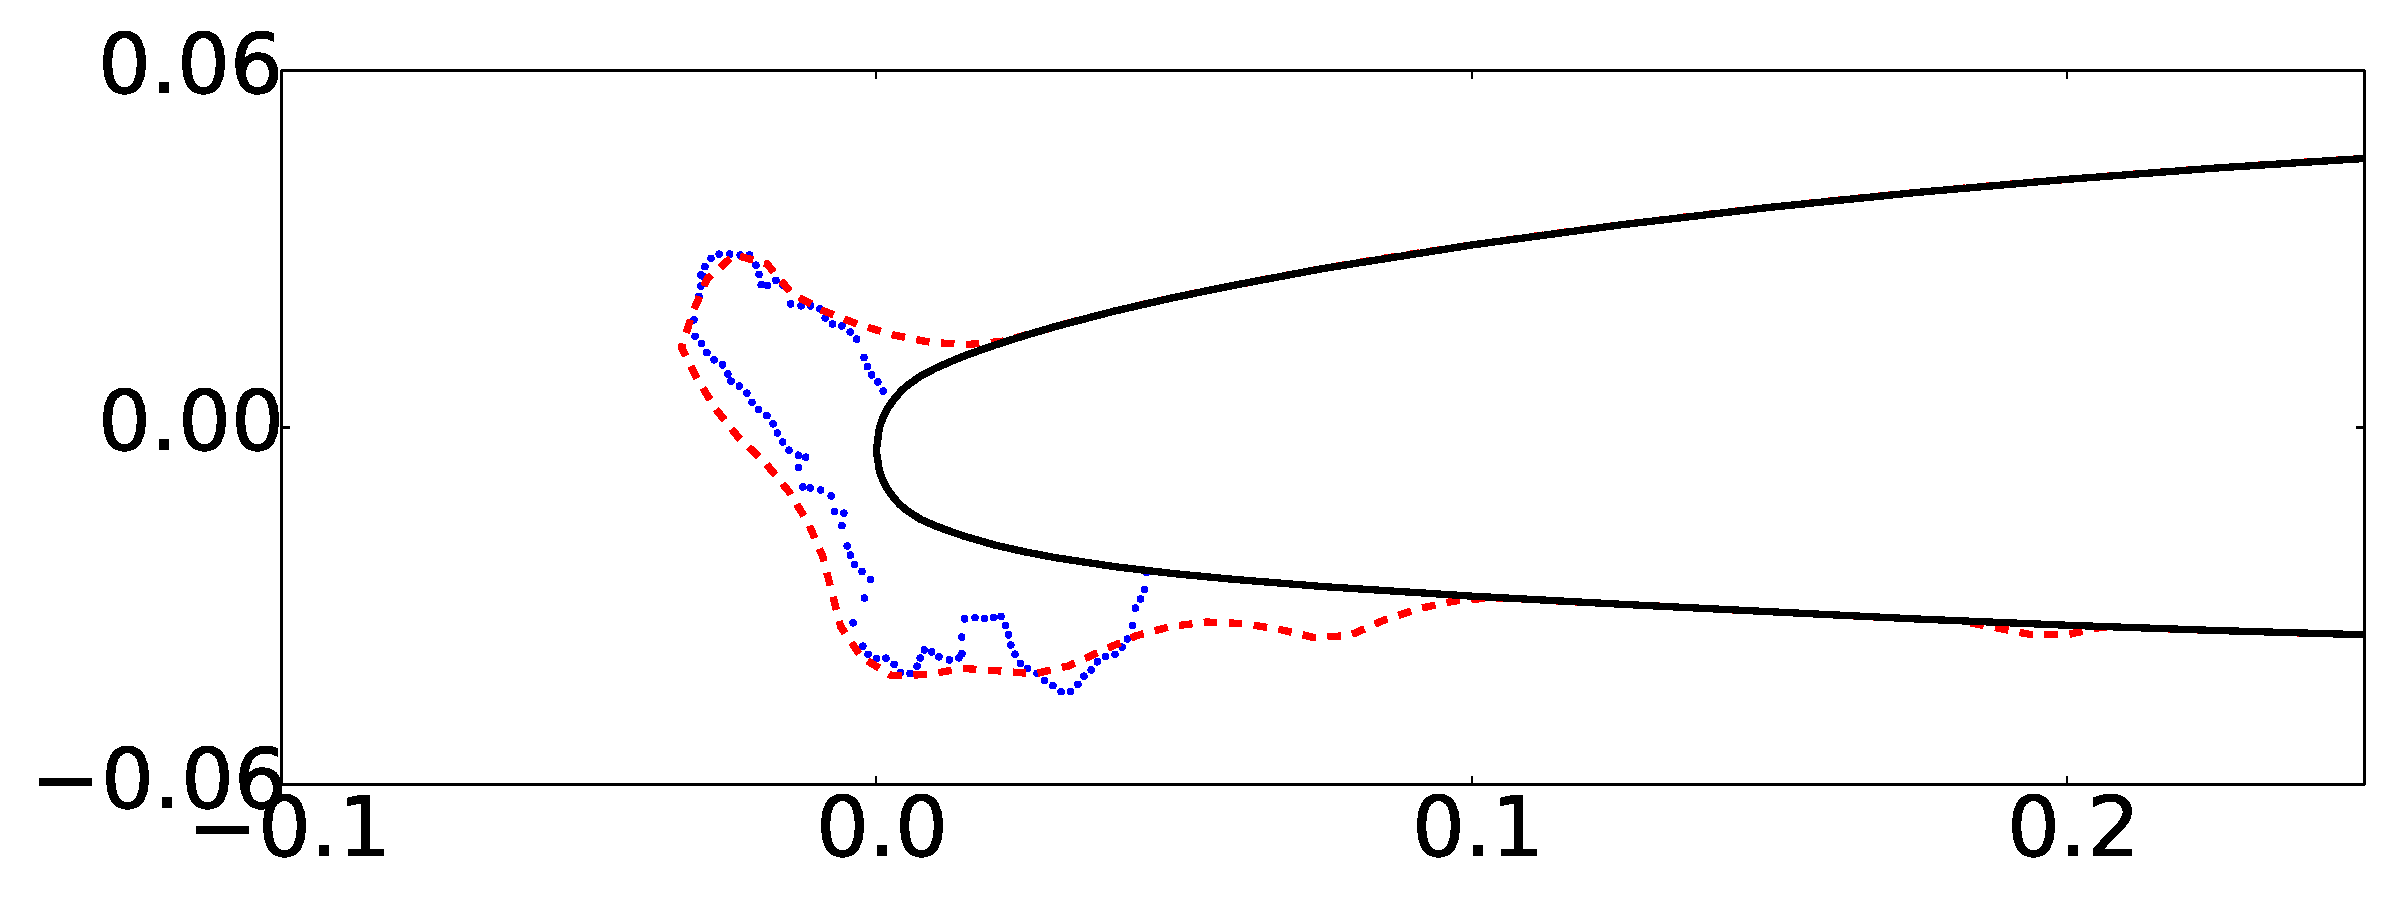
\includegraphics[width=1\textwidth]{ReconstructionE3} \\
    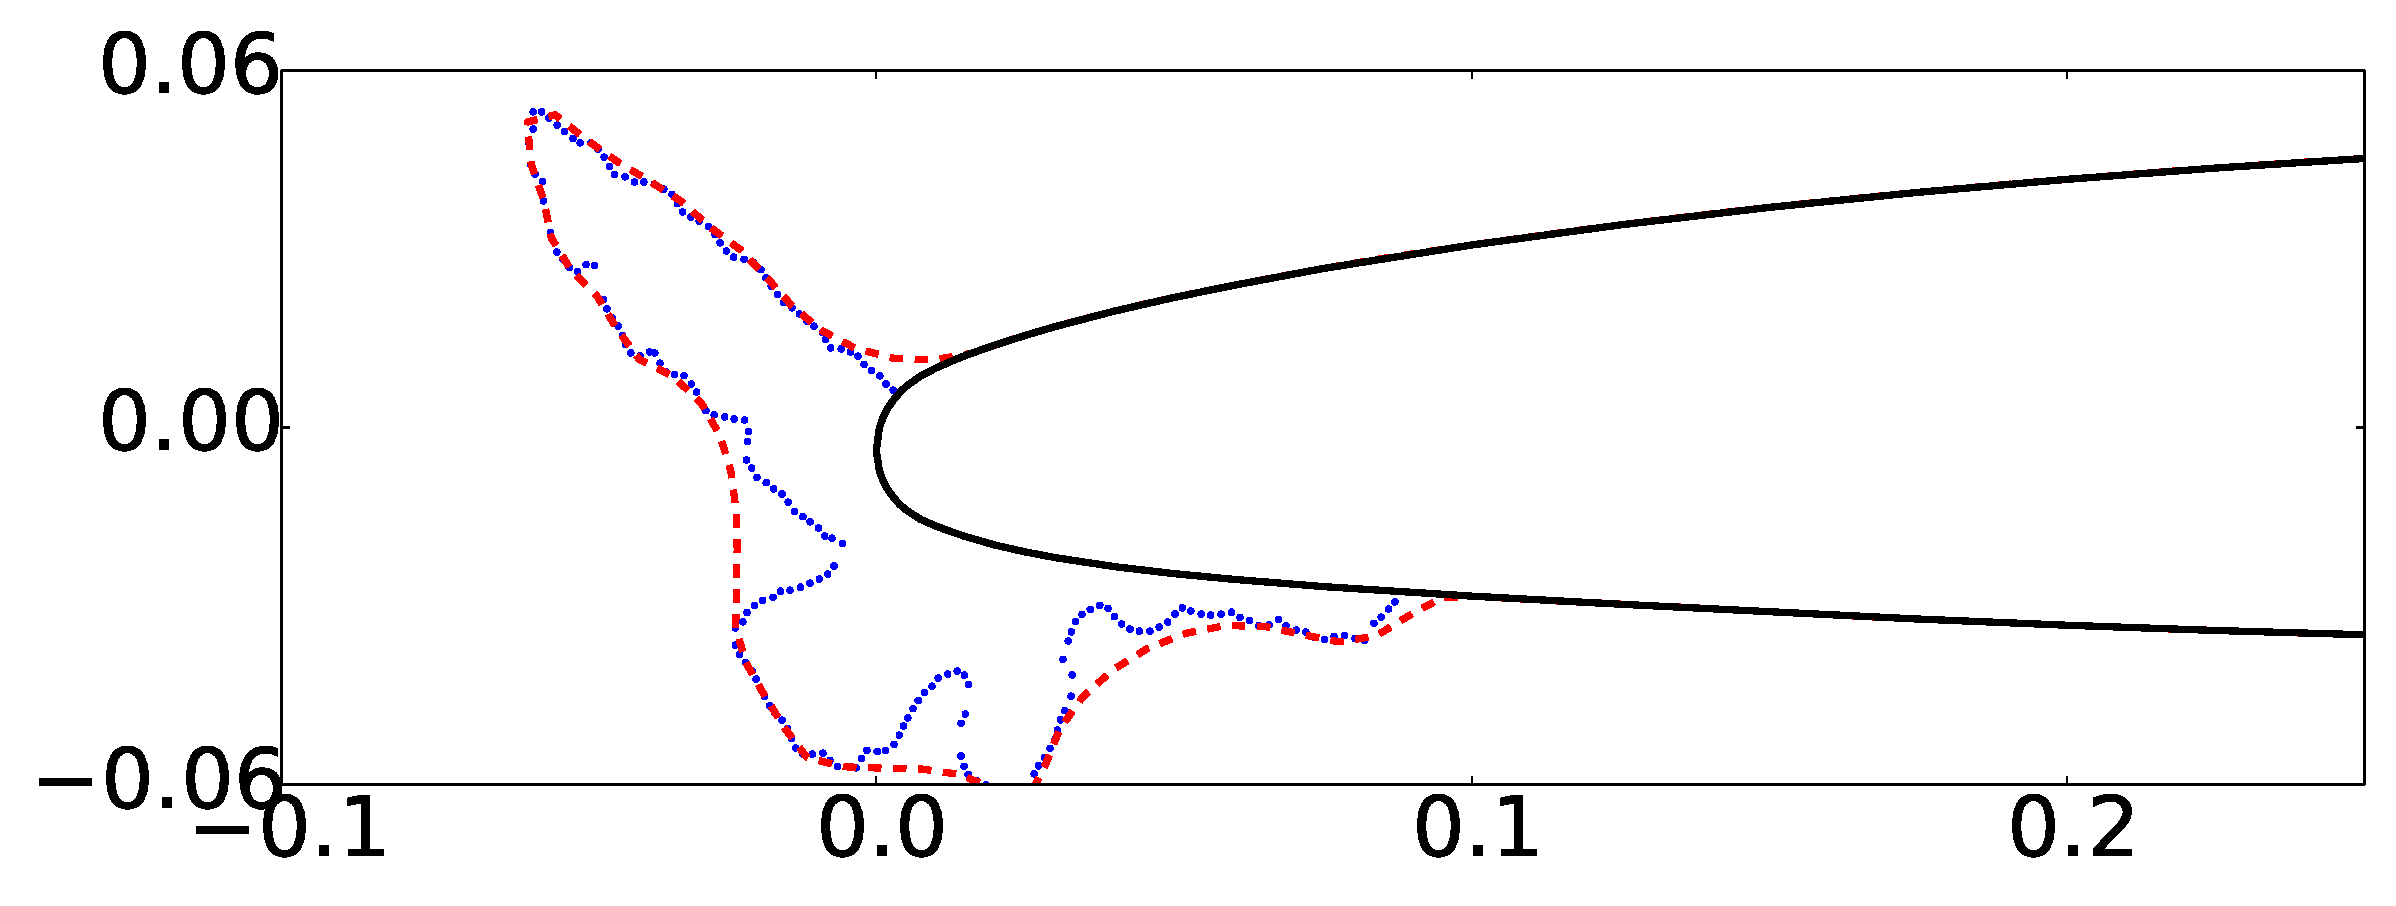
\includegraphics[width=1\textwidth]{ReconstructionE4} \\
\end{columns}
\begin{center}
{\bf Ice Reconstructions}
\end{center}
\end{frame}
\begin{frame}
\frametitle{Preliminary Findings}
\label{sec-4-4}


\begin{figure}
  \centering
  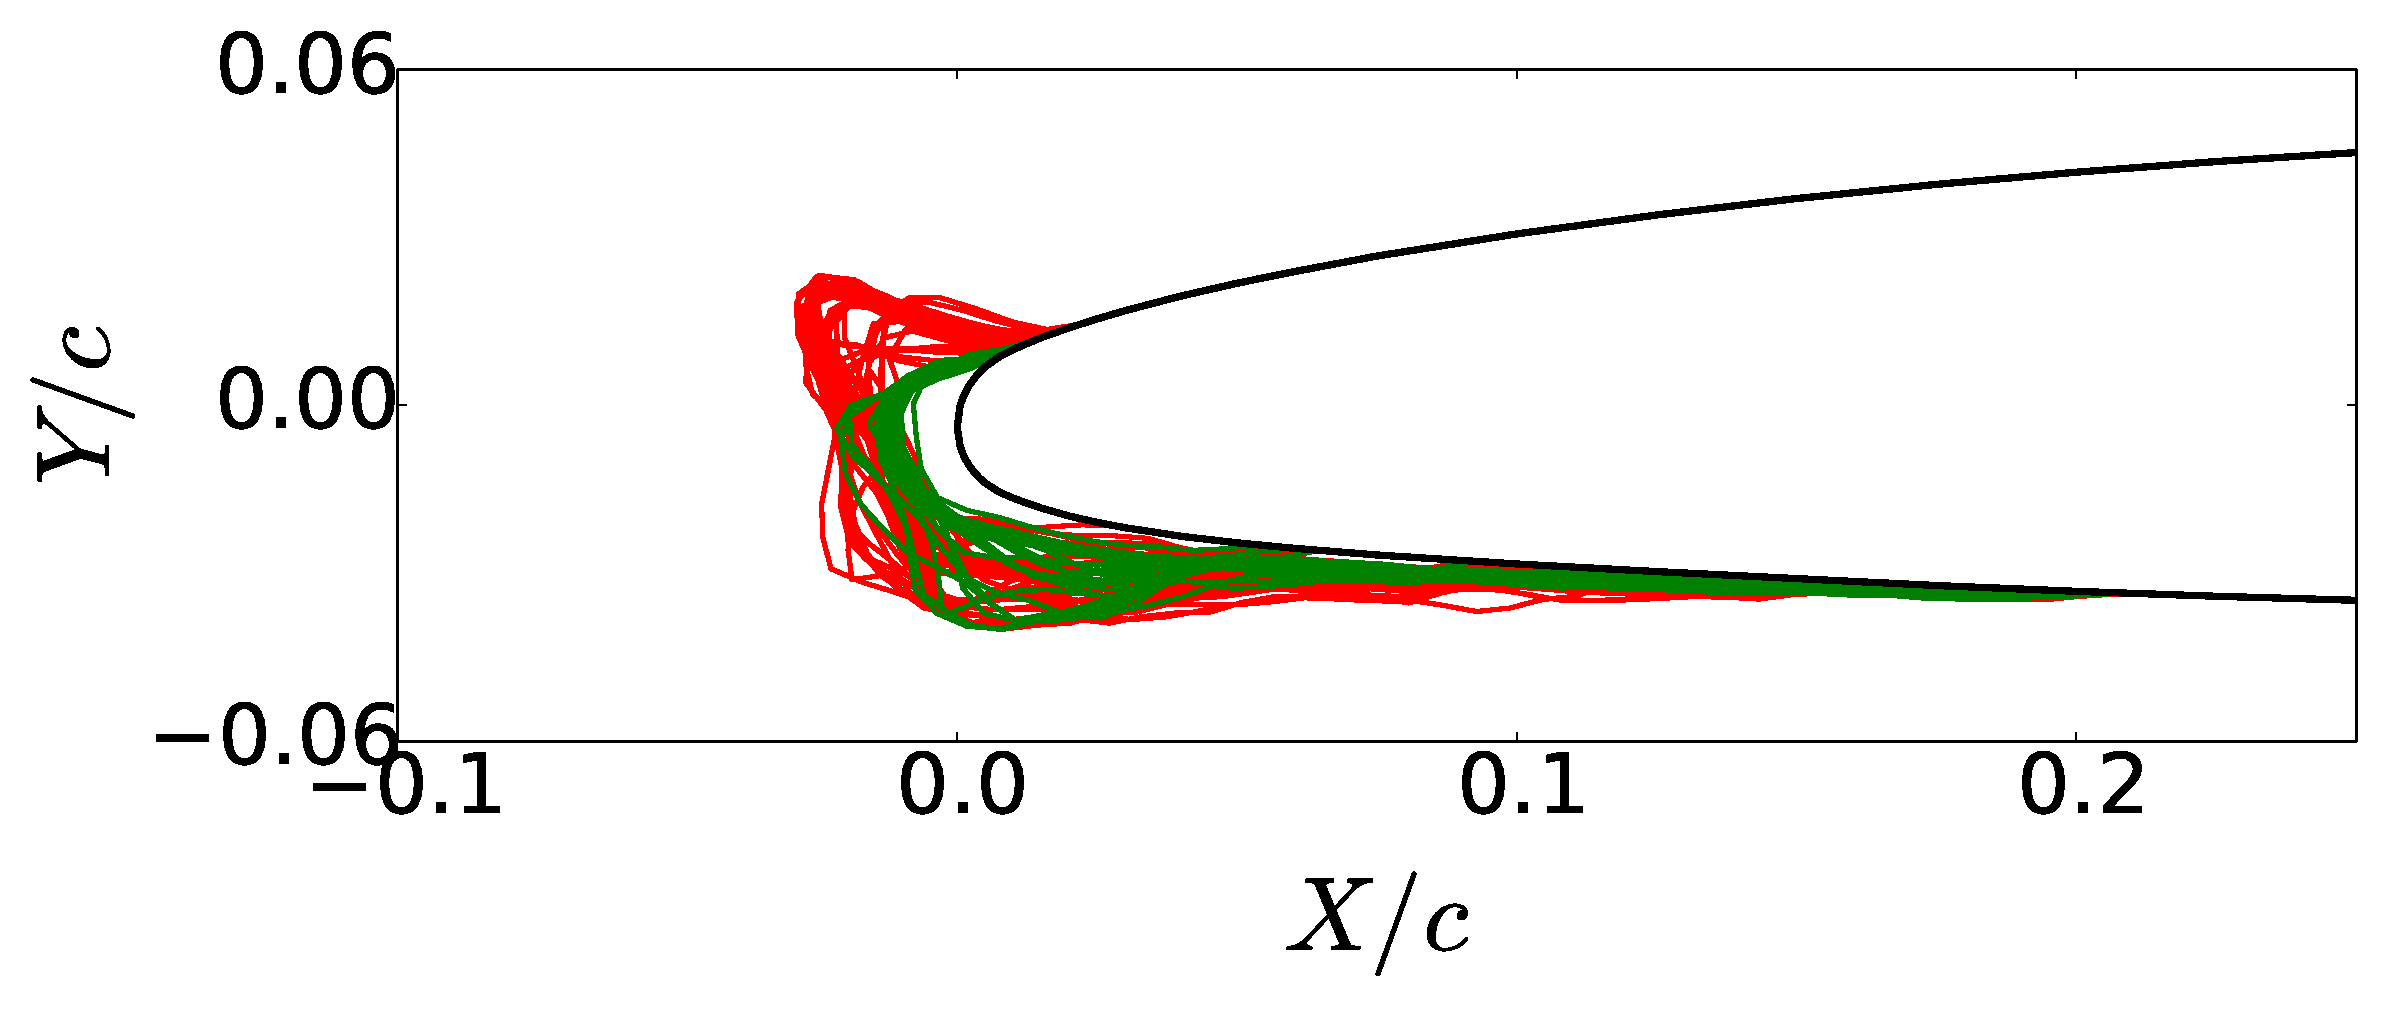
\includegraphics[width=0.7\textwidth]{GoodBadHornExamps}
\end{figure}

\begin{itemize}
\item \textbf{Green:} Horns which produce upper 10$\%$ of $C_L$
\begin{itemize}
\item Lower amounts of ice accumulation
\item Ice mass concentrated on lower surface
\end{itemize}
\item \textbf{Red:} Horns which produce lower 10$\%$ of $C_L$
\begin{itemize}
\item Higher amounts of ice accumulation
\item Ice mass forms sharp upper surface horn
\end{itemize}
\item Results derived from $\sim 5,500$ sparse grid evaluations
\item More sparse grid evaluations are currently underway to produce a
  faithful, converged PCE surrogate
\end{itemize}
\end{frame}
\section{Computational-Based UQ}
\label{sec-5}
\begin{frame}
\frametitle{Motivation}
\label{sec-5-1}

\begin{itemize}
\item \textbf{Investigate uncertainty in the physical process of icing}
\begin{itemize}
\item Distribution of droplet diameters affects collection efficiency
\begin{itemize}
\item How sensitive is collection efficiency to perturbations in MVD distribution?
\end{itemize}
\item Surface tension of SLDs varies with their temperature
\begin{itemize}
\item Can affect impingement details $\rightarrow$ collection efficiency
\item Can affect surface roughness
\end{itemize}
\item Surface roughness could vary as SLDs impinge and freeze
\begin{itemize}
\item Can affect local convective heat transfer
\item Can influence local rate of ice accretion
\end{itemize}
\end{itemize}
\end{itemize}
\end{frame}
\begin{frame}
\frametitle{Droplet Diameter Distribution}
\label{sec-5-2}

\begin{columns}[c]
  \column{0.5\textwidth}
    \centering
    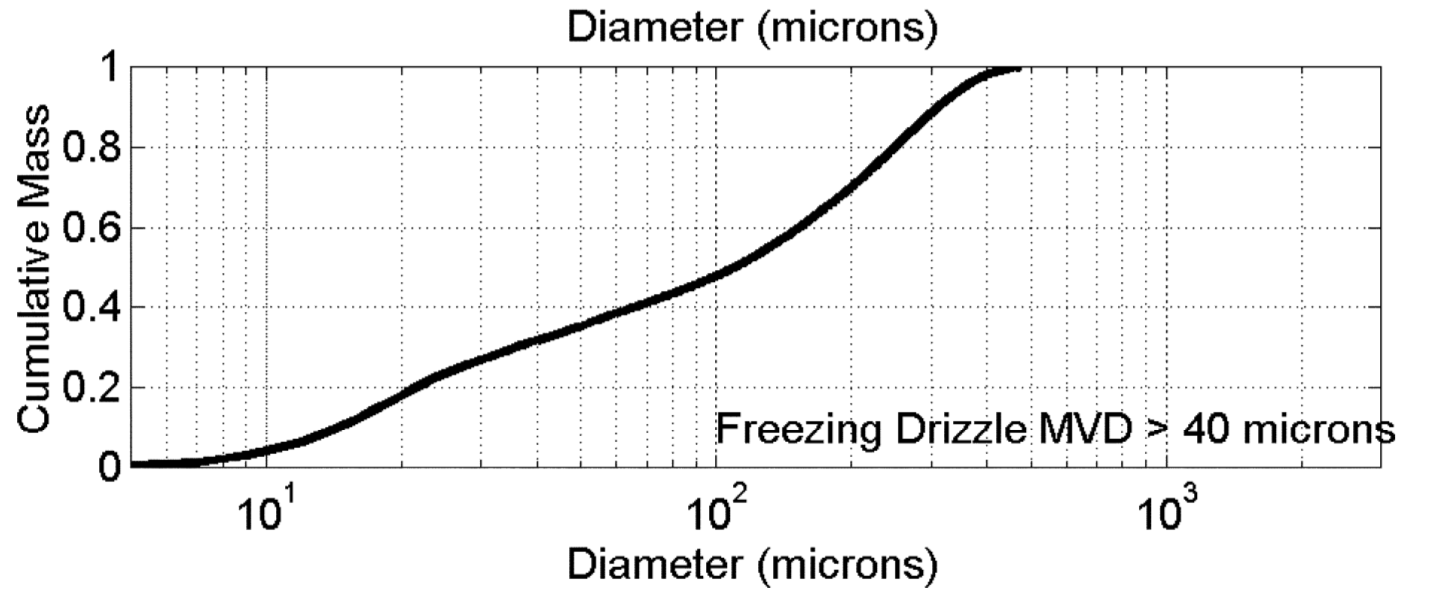
\includegraphics[width=1\textwidth]{FAADropletDist1} \\
    {\bf Freezing Drizzle MVD PDF}
  \column{0.5\textwidth}
    \centering
    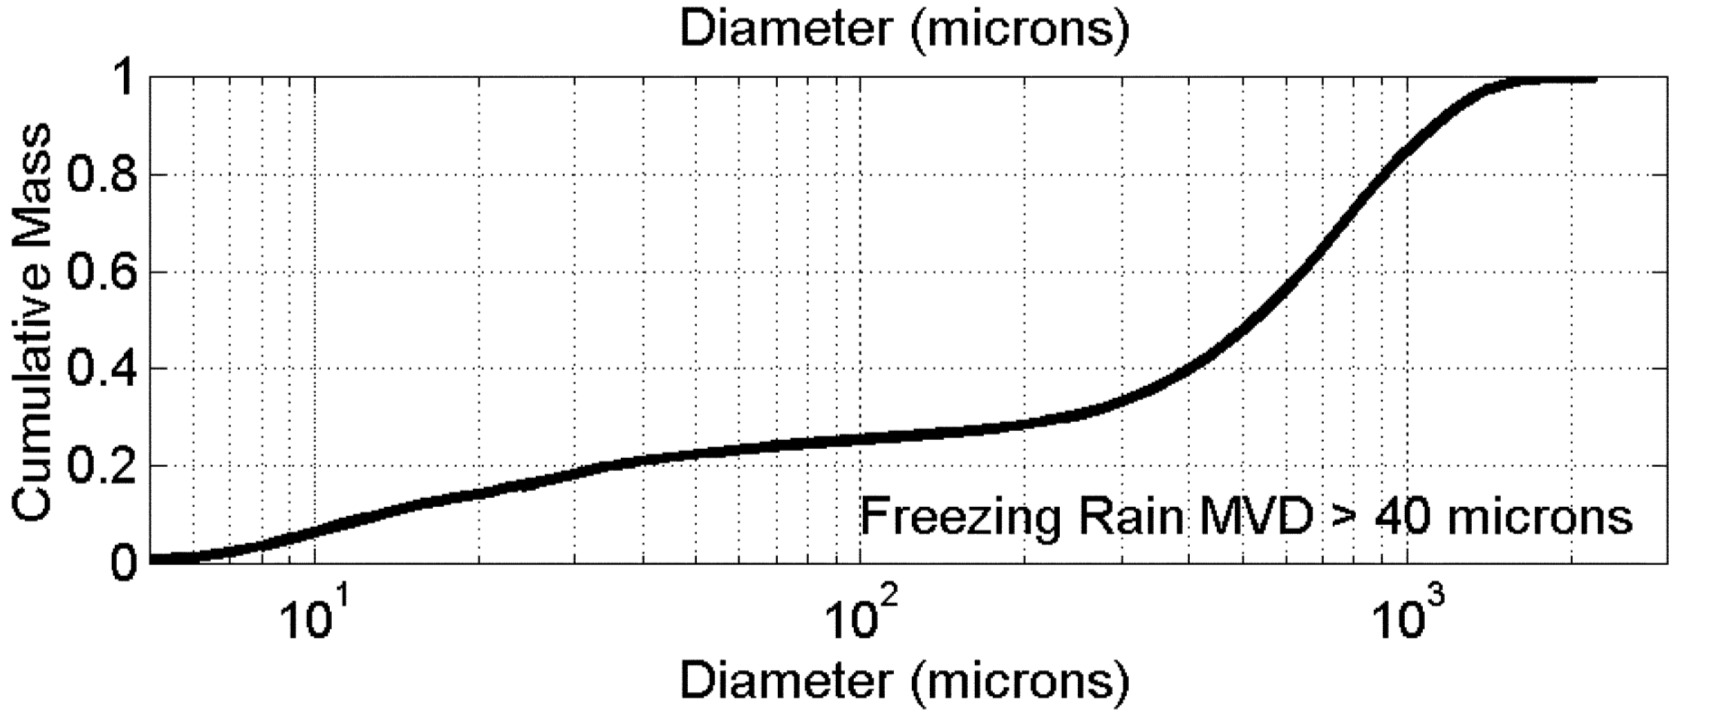
\includegraphics[width=1\textwidth]{FAADropletDist2} \\
    {\bf Freezing Rain MVD PDF}
\end{columns}

\begin{itemize}
\item Several MVD distributions exist for different flight conditions \footnote{Airplane and Engine Certification Requirements in
Supercooled Large Drop, Mixed Phase, and Ice Crystal Icing Conditions;
Final Rule. Federal Register, Vol. 79, No. 213.
 }
\item Each gives a different collection efficiency
\item How sensitive are collection efficiency and ice shape to perturbations in MVD distribution?
\end{itemize}
\end{frame}
\begin{frame}
\frametitle{Surface Tension vs. Temperature}
\label{sec-5-3}

\begin{figure}
  \centering
  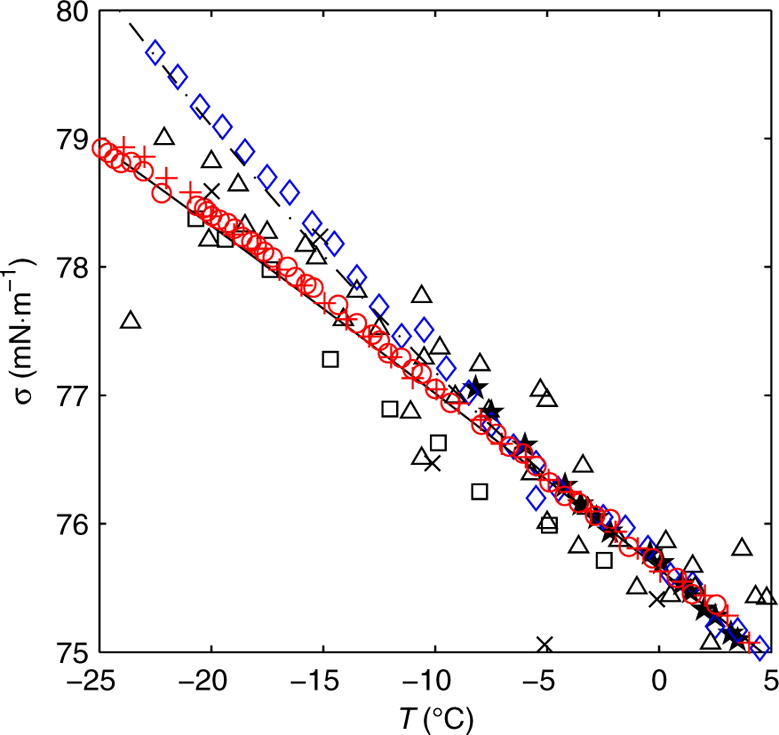
\includegraphics[width=0.33\textwidth]{SurfaceTensionVsTemp.jpeg} \\
  {\bf Surface Tension vs. Temperature}
\end{figure}

\begin{itemize}
\item Surface tension of SLDs varies with temperature \footnote{Hruby, J. et. al. Surface Tension of Supercooled Water:
No Inflection Point down -25 Degrees
Celsius. J. Phys. Chem. Lett. 2014, 5, 425-28.
 }
\item Varying surface tension can affect collection efficiency
\item Higher surface tension may give rise to ``beading'' on surface
  (vs. deposition into film), which could affect surface roughness
\end{itemize}
\end{frame}
\begin{frame}
\frametitle{Roughness Variations}
\label{sec-5-4}

\begin{figure}
  \centering
  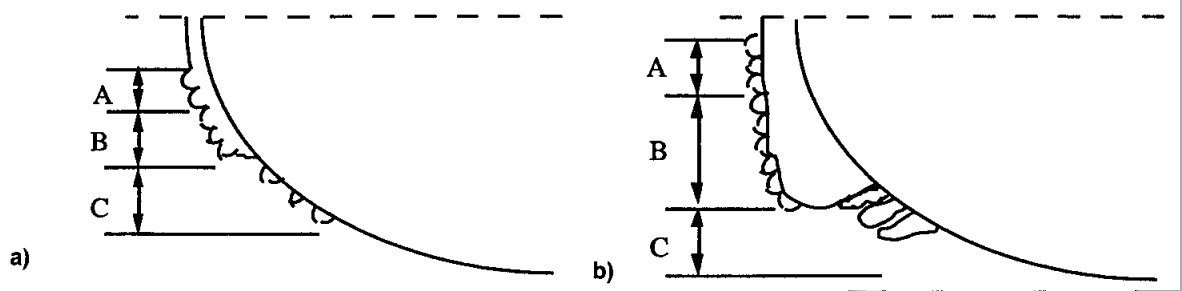
\includegraphics[width=1\textwidth]{IcingRoughness.png} \\
  {\bf Roughness Growth}
\end{figure}

\begin{itemize}
\item \textbf{Surface roughness varies with parameters} \footnote{Shin, J. Characteristics of Surface Roughness Associated
with Leading-Edge Ice Accretion. Journal of Aircraft, Vol. 33, No.2,
April 1996.
 }
\begin{itemize}
\item Roughness height increases with temperature and LWC
\item Beginning of roughness varies with temperature, speed, LWC
\end{itemize}
\item \textbf{Surface roughness affects shape/aerodynamics} \footnotemark[12]
\begin{itemize}
\item Roughness elements probably protrude out of boundary layer and cause transition
\item Irregularity of shape should be calculated by ice accretion code, not treated as part of roughness model
\end{itemize}
\end{itemize}
\end{frame}
\begin{frame}
\frametitle{Airfoil Icing Code Flowchart}
\label{sec-5-5}

\fontsize{7}\selectfont
% Define the layers to draw the diagram
\pgfdeclarelayer{background}
\pgfdeclarelayer{foreground}
\pgfsetlayers{background,main,foreground}

% Define block styles used later

\tikzstyle{sensor}=[draw, fill=blue!20, text width=5em, 
    text centered, minimum height=2.5em,drop shadow]
\tikzstyle{ann} = [above, text width=5em, text centered]
\tikzstyle{wa} = [sensor, text width=7.5em, fill=blue!20, 
    minimum height=3em, rounded corners, drop shadow]

% Define distances for bordering
\def\blockdist{2.3}
\def\edgedist{2.5}

\begin{tikzpicture}
    \node (CleanAirfoil) [wa]  {Clean Airfoil Geometry};
    \path (CleanAirfoil)+(4,2.5) node (FlowSolver) [wa] {Mesh/Flow Solver};
    \path (FlowSolver)+(0,-1.25) node (Droplet) [wa] {Droplet\\Advection Module};
    \path (Droplet)+(0,-1.25) node (ThermoModule) [wa] {Thermodynamic Module};
    \path (ThermoModule)+(0,-1.25) node (IcedAirfoil) [wa] {Iced Airfoil Geometry};
    \path (CleanAirfoil)+(8,0) node (FinalAirfoil) [wa] {Final Iced Airfoil Geometry};

    \path [draw, ->, thick] (CleanAirfoil.north) |- node [above] {} (FlowSolver.west);
    \path [draw, ->, thick] (FlowSolver.south) -- node [below] {} (Droplet.north);
    \path [draw, ->, thick] (Droplet.south) -- node [below] {} (ThermoModule.north);
    \path [draw, ->, thick] (ThermoModule.south) -- node [below] {} (IcedAirfoil.north);
    \path [draw, ->, thick] (IcedAirfoil.east) -| node [above] {} (FinalAirfoil.south);
    \path [draw, ->, thick] (IcedAirfoil.east) -- ++(0.75,0cm) |- node [above]
                      {} (FlowSolver.east);

    \begin{pgfonlayer}{background}
        \path (FlowSolver.west)+(-1,1) node (a) {};
        \path (IcedAirfoil.east)+(1,-1) node (b) {};
        \path[fill=orange!20,rounded corners, draw=black!50, dashed] (a) rectangle (b);
            
    \end{pgfonlayer}

\end{tikzpicture}
\end{frame}
\begin{frame}
\frametitle{Droplet Advection}
\label{sec-5-6}

\begin{equation*}
  \begin{align}
    \frac{d \bv{x}}{d t} &= \bv{v} \\
    m \frac{d \bv{v}}{d t} &= \frac{1}{2} \rho_g C_D \pi r^2 ||\bv{v_g} - \bv{v}|| (\bv{v_g} - \bv{v}) + m \bv{g}
  \end{align}
\end{equation}

\begin{columns}[c]
  \column{0.5\textwidth}
    \centering
    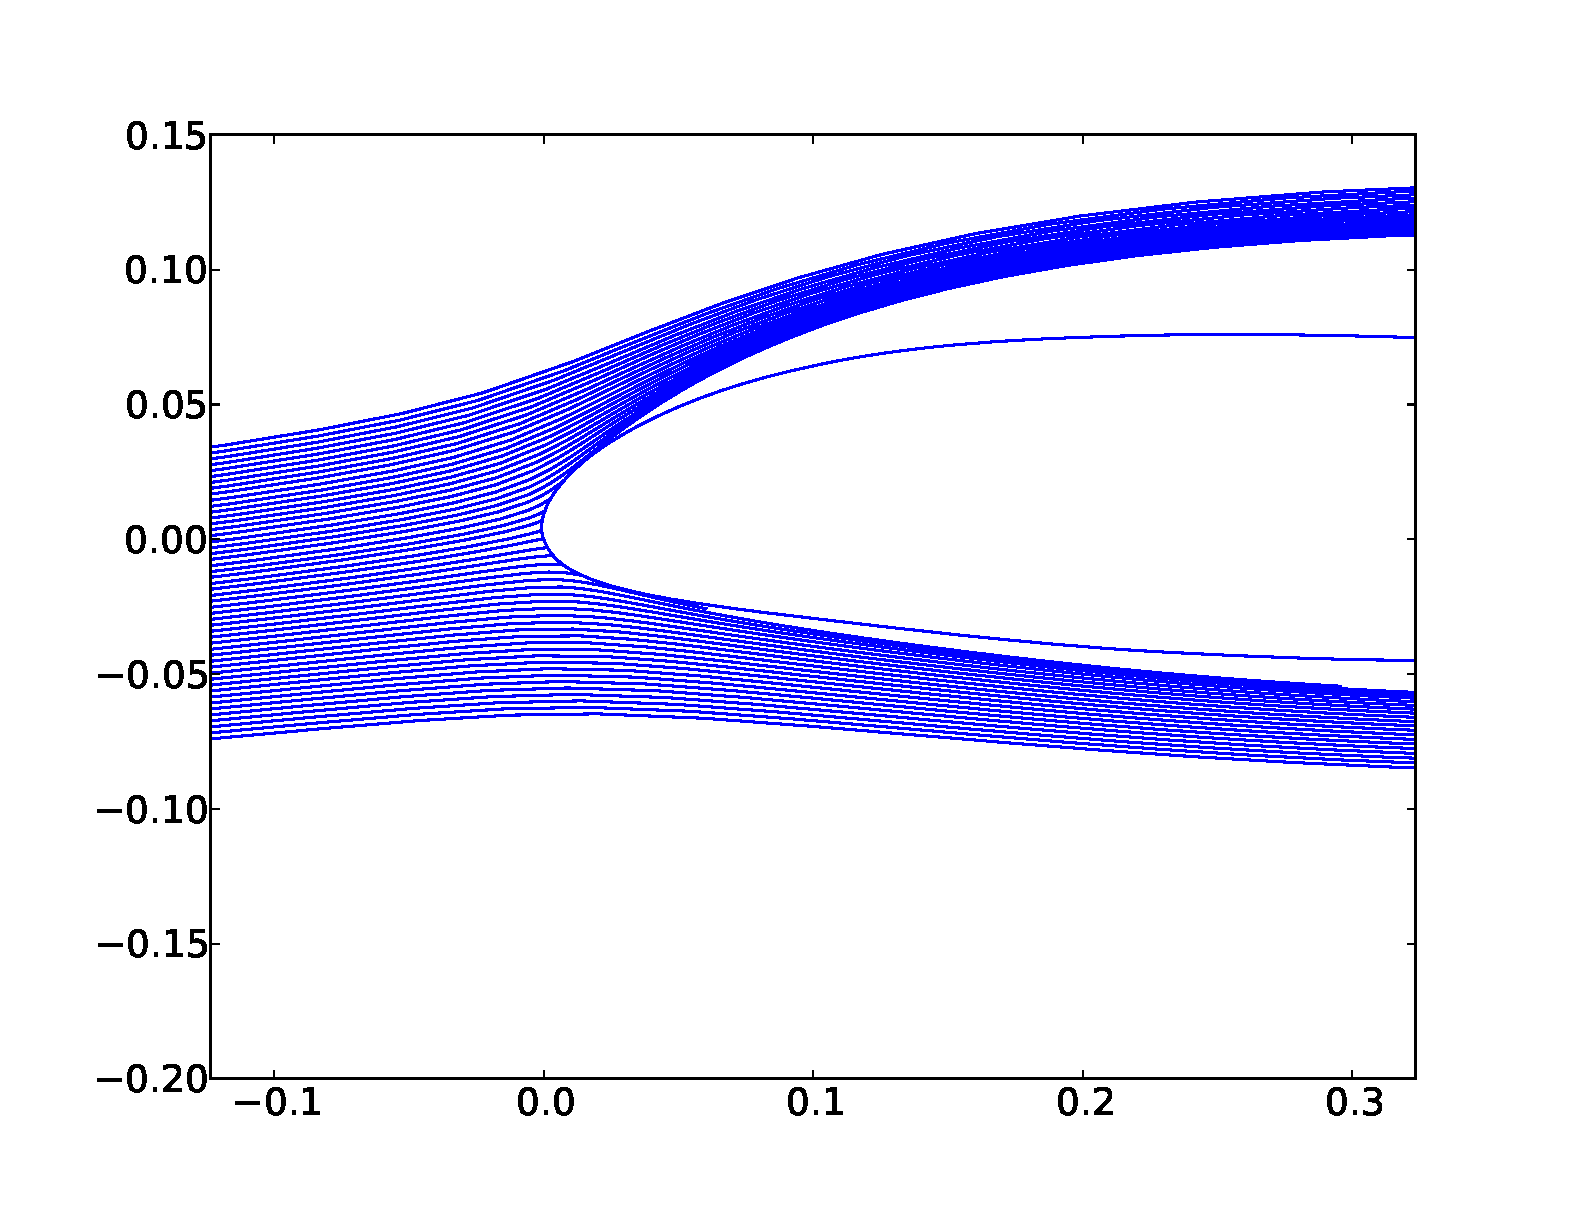
\includegraphics[width=1\textwidth]{ExampleR10em6} \\
    {\bf R = 10$\mu$m}
  \column{0.5\textwidth}
    \centering
    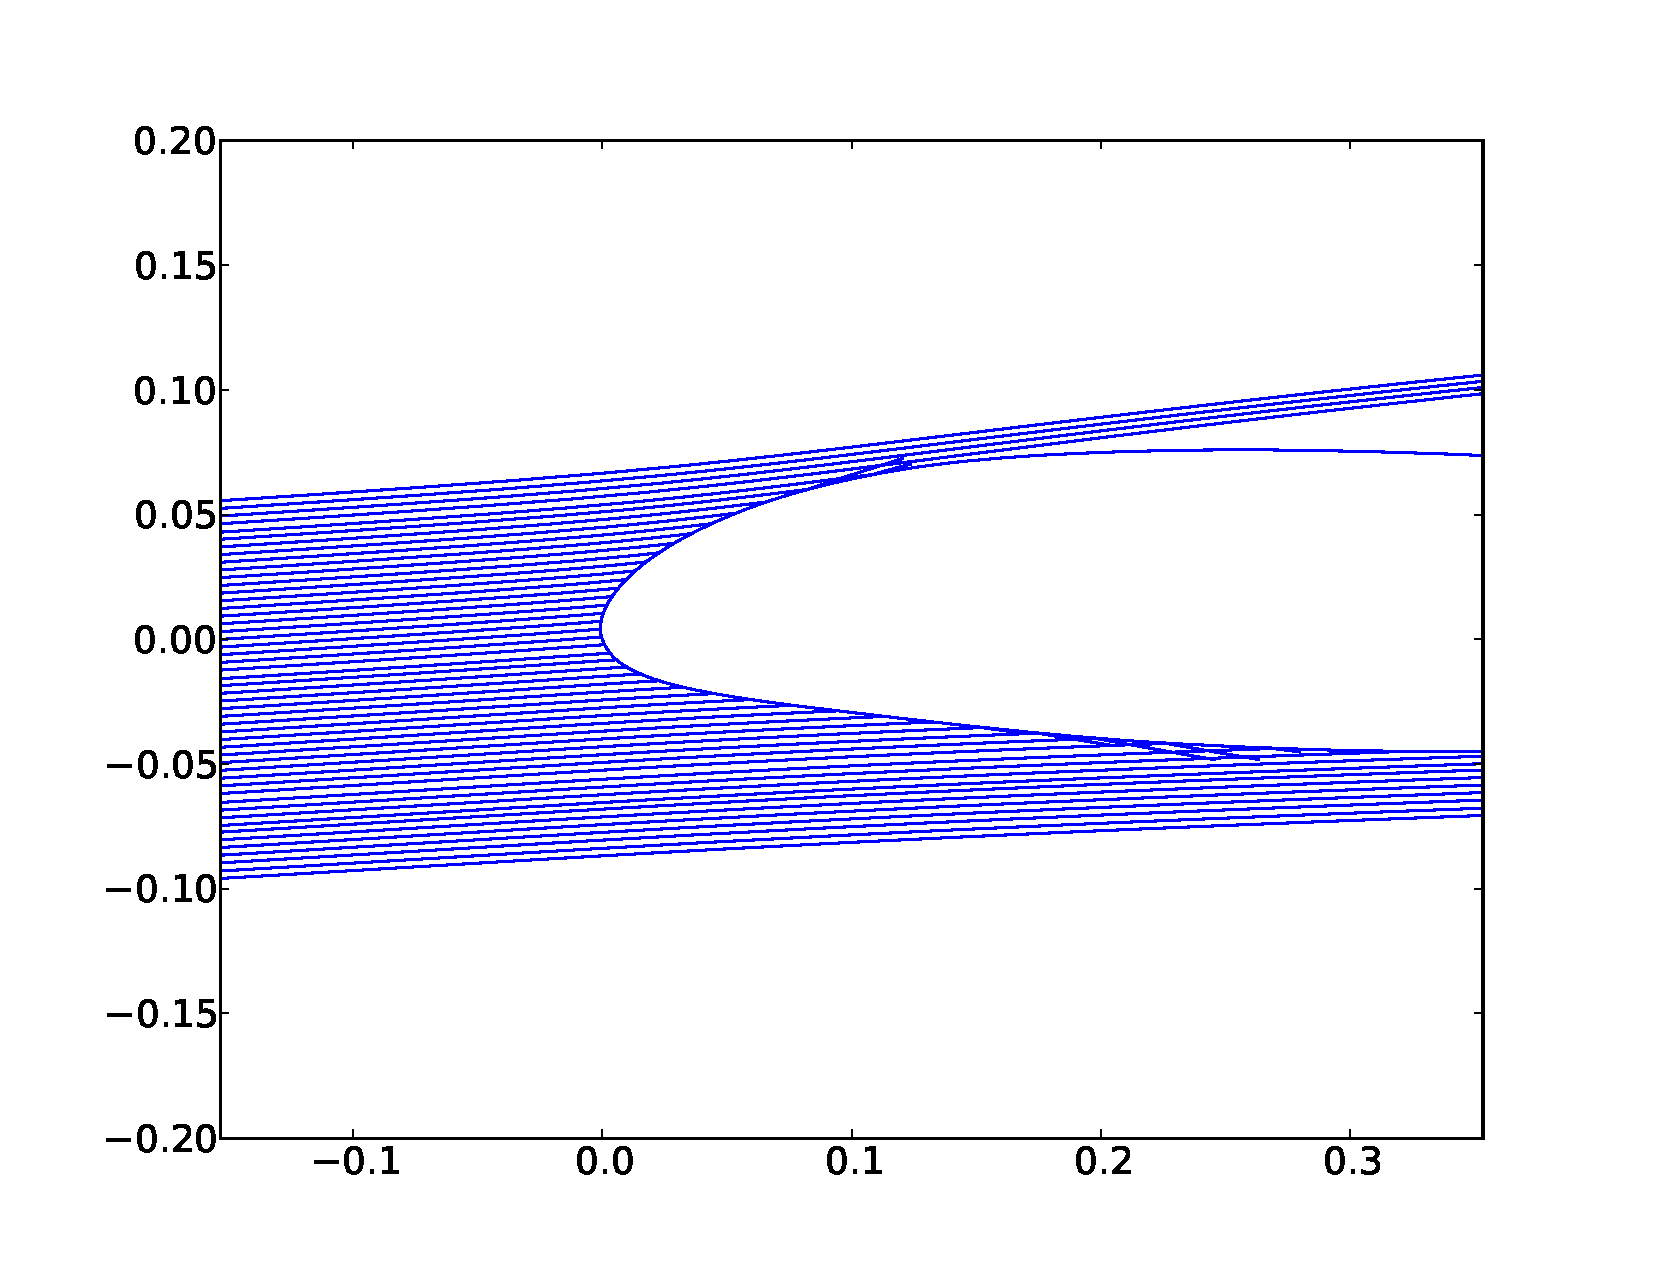
\includegraphics[width=1\textwidth]{ExampleR100em6} \\
    {\bf R = 100$\mu$m}
\end{columns}
\end{frame}
\begin{frame}
\frametitle{Preliminary Intermediate Results: Mass Flux}
\label{sec-5-7}


\begin{columns}[c]
  \column{0.5\textwidth}
    \centering
    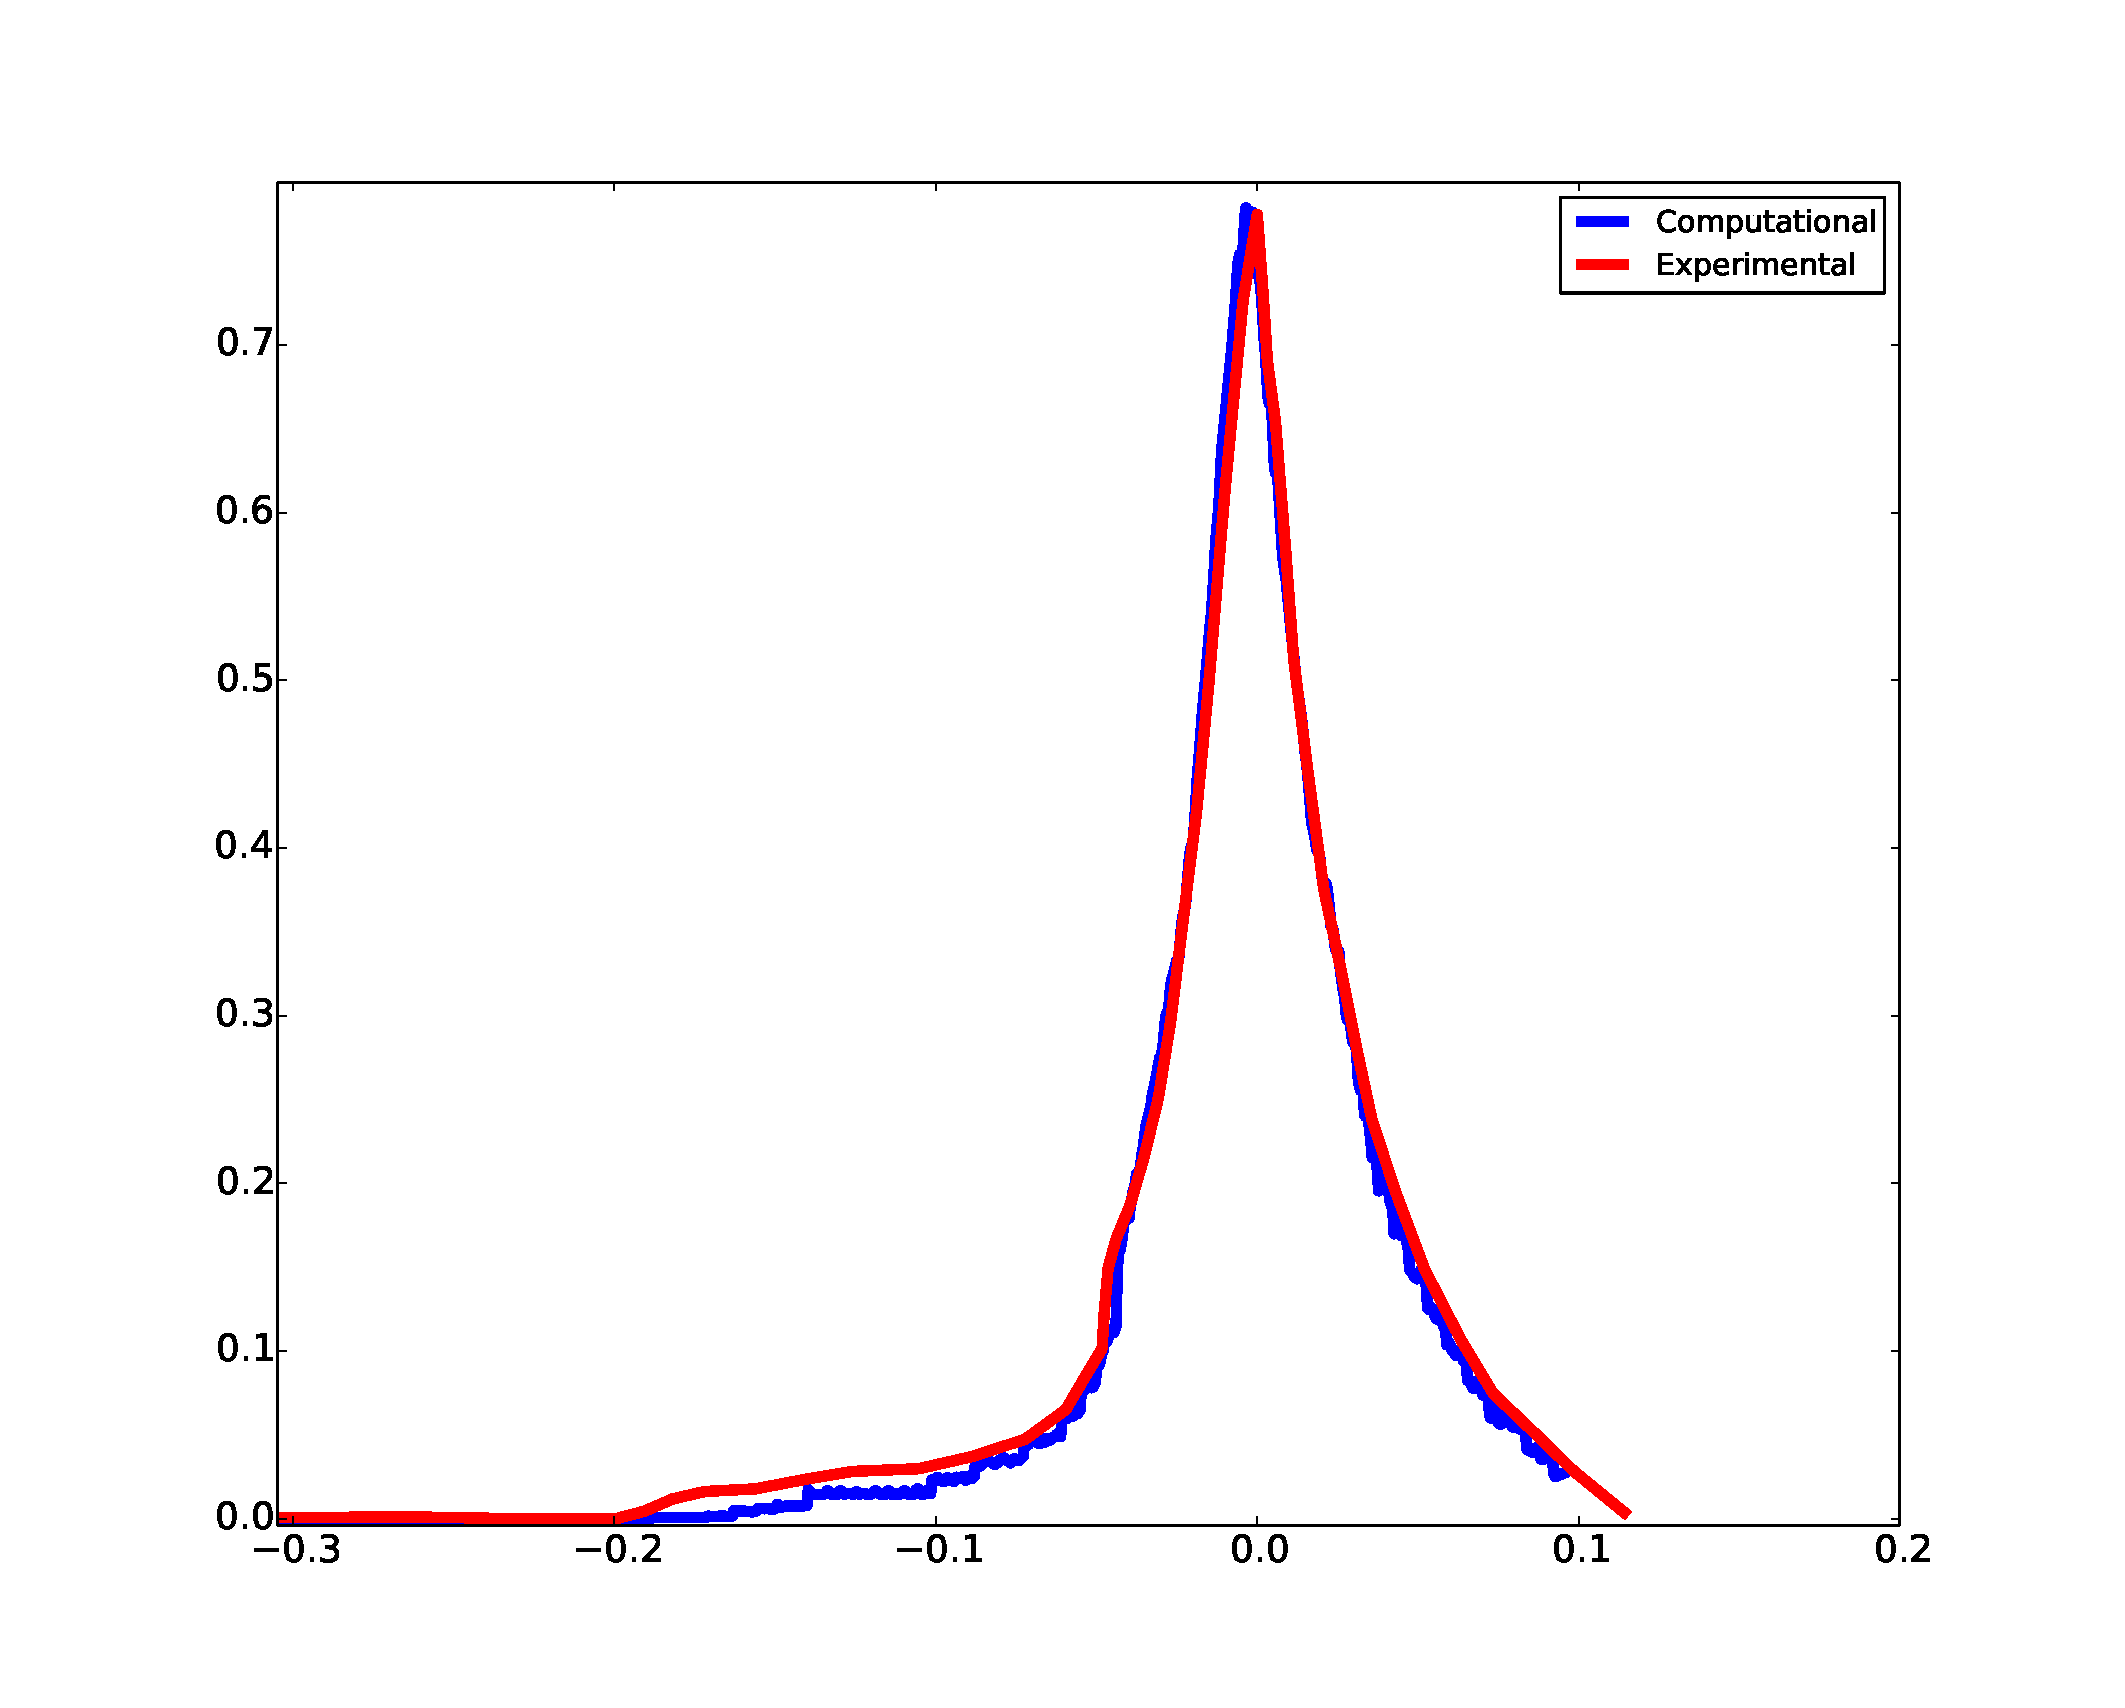
\includegraphics[width=0.65\textwidth]{MVD52} \\
    {\bf MVD 52} \\
    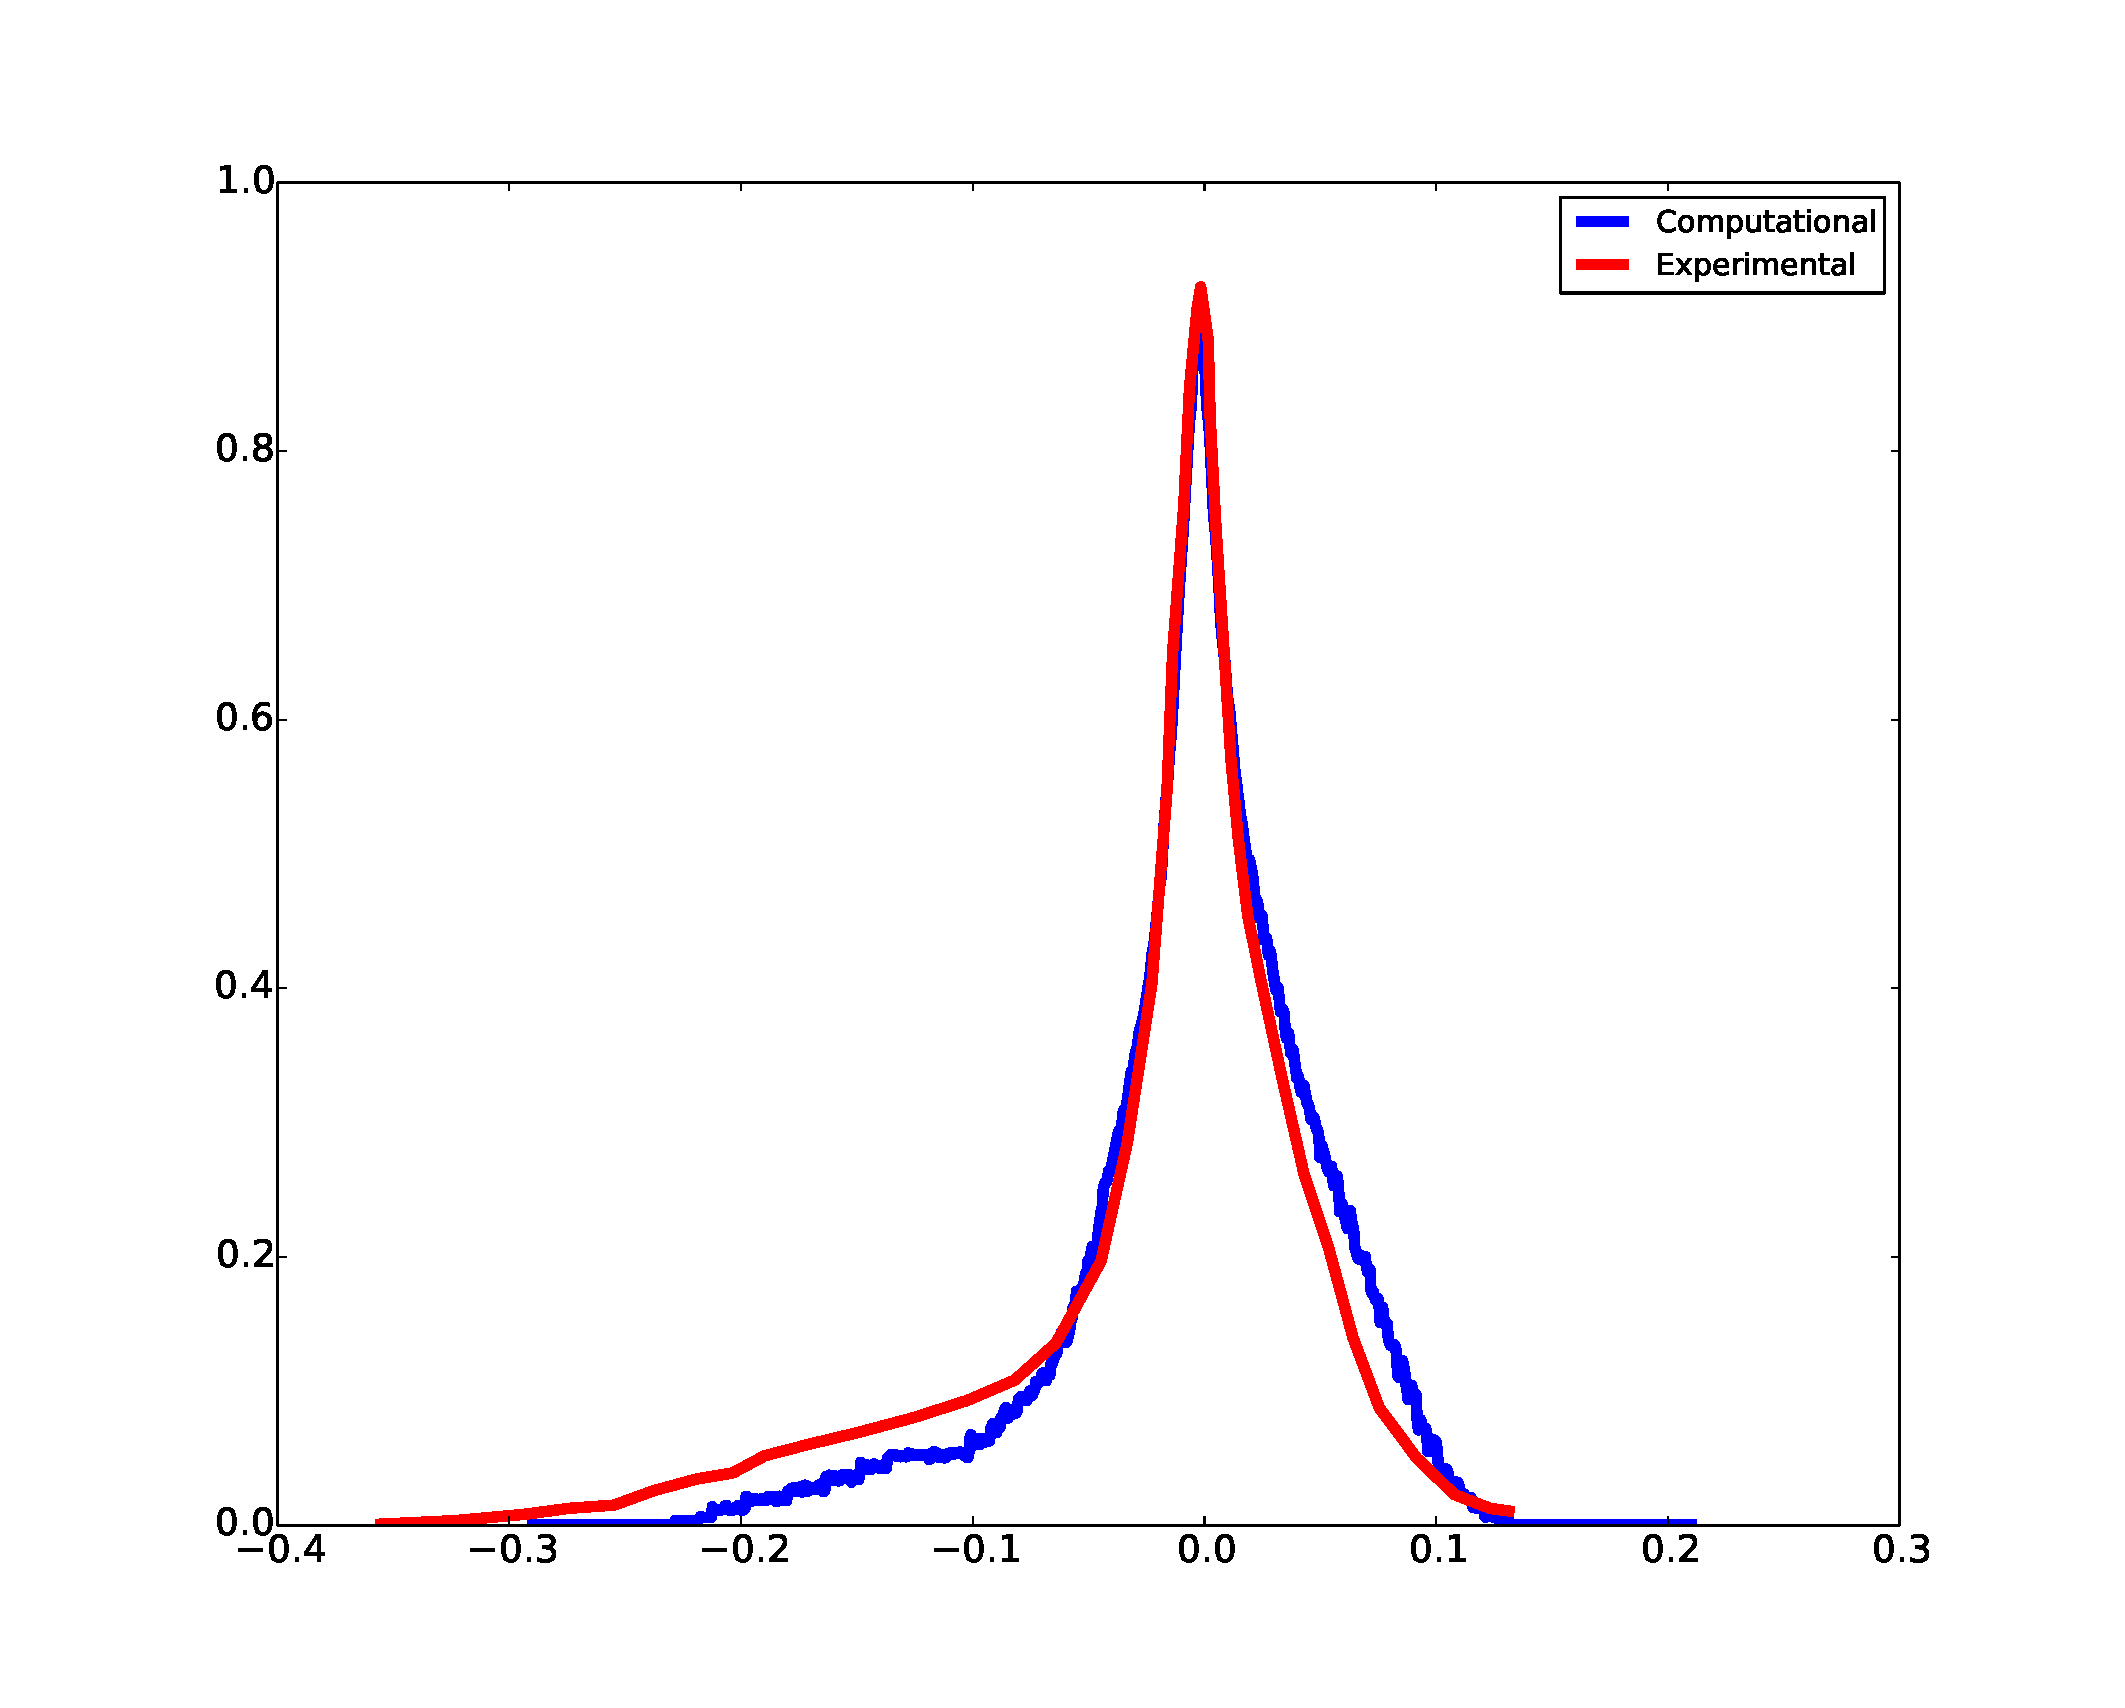
\includegraphics[width=0.65\textwidth]{MVD154} \\
    {\bf MVD 154}
  \column{0.5\textwidth}
    \centering
    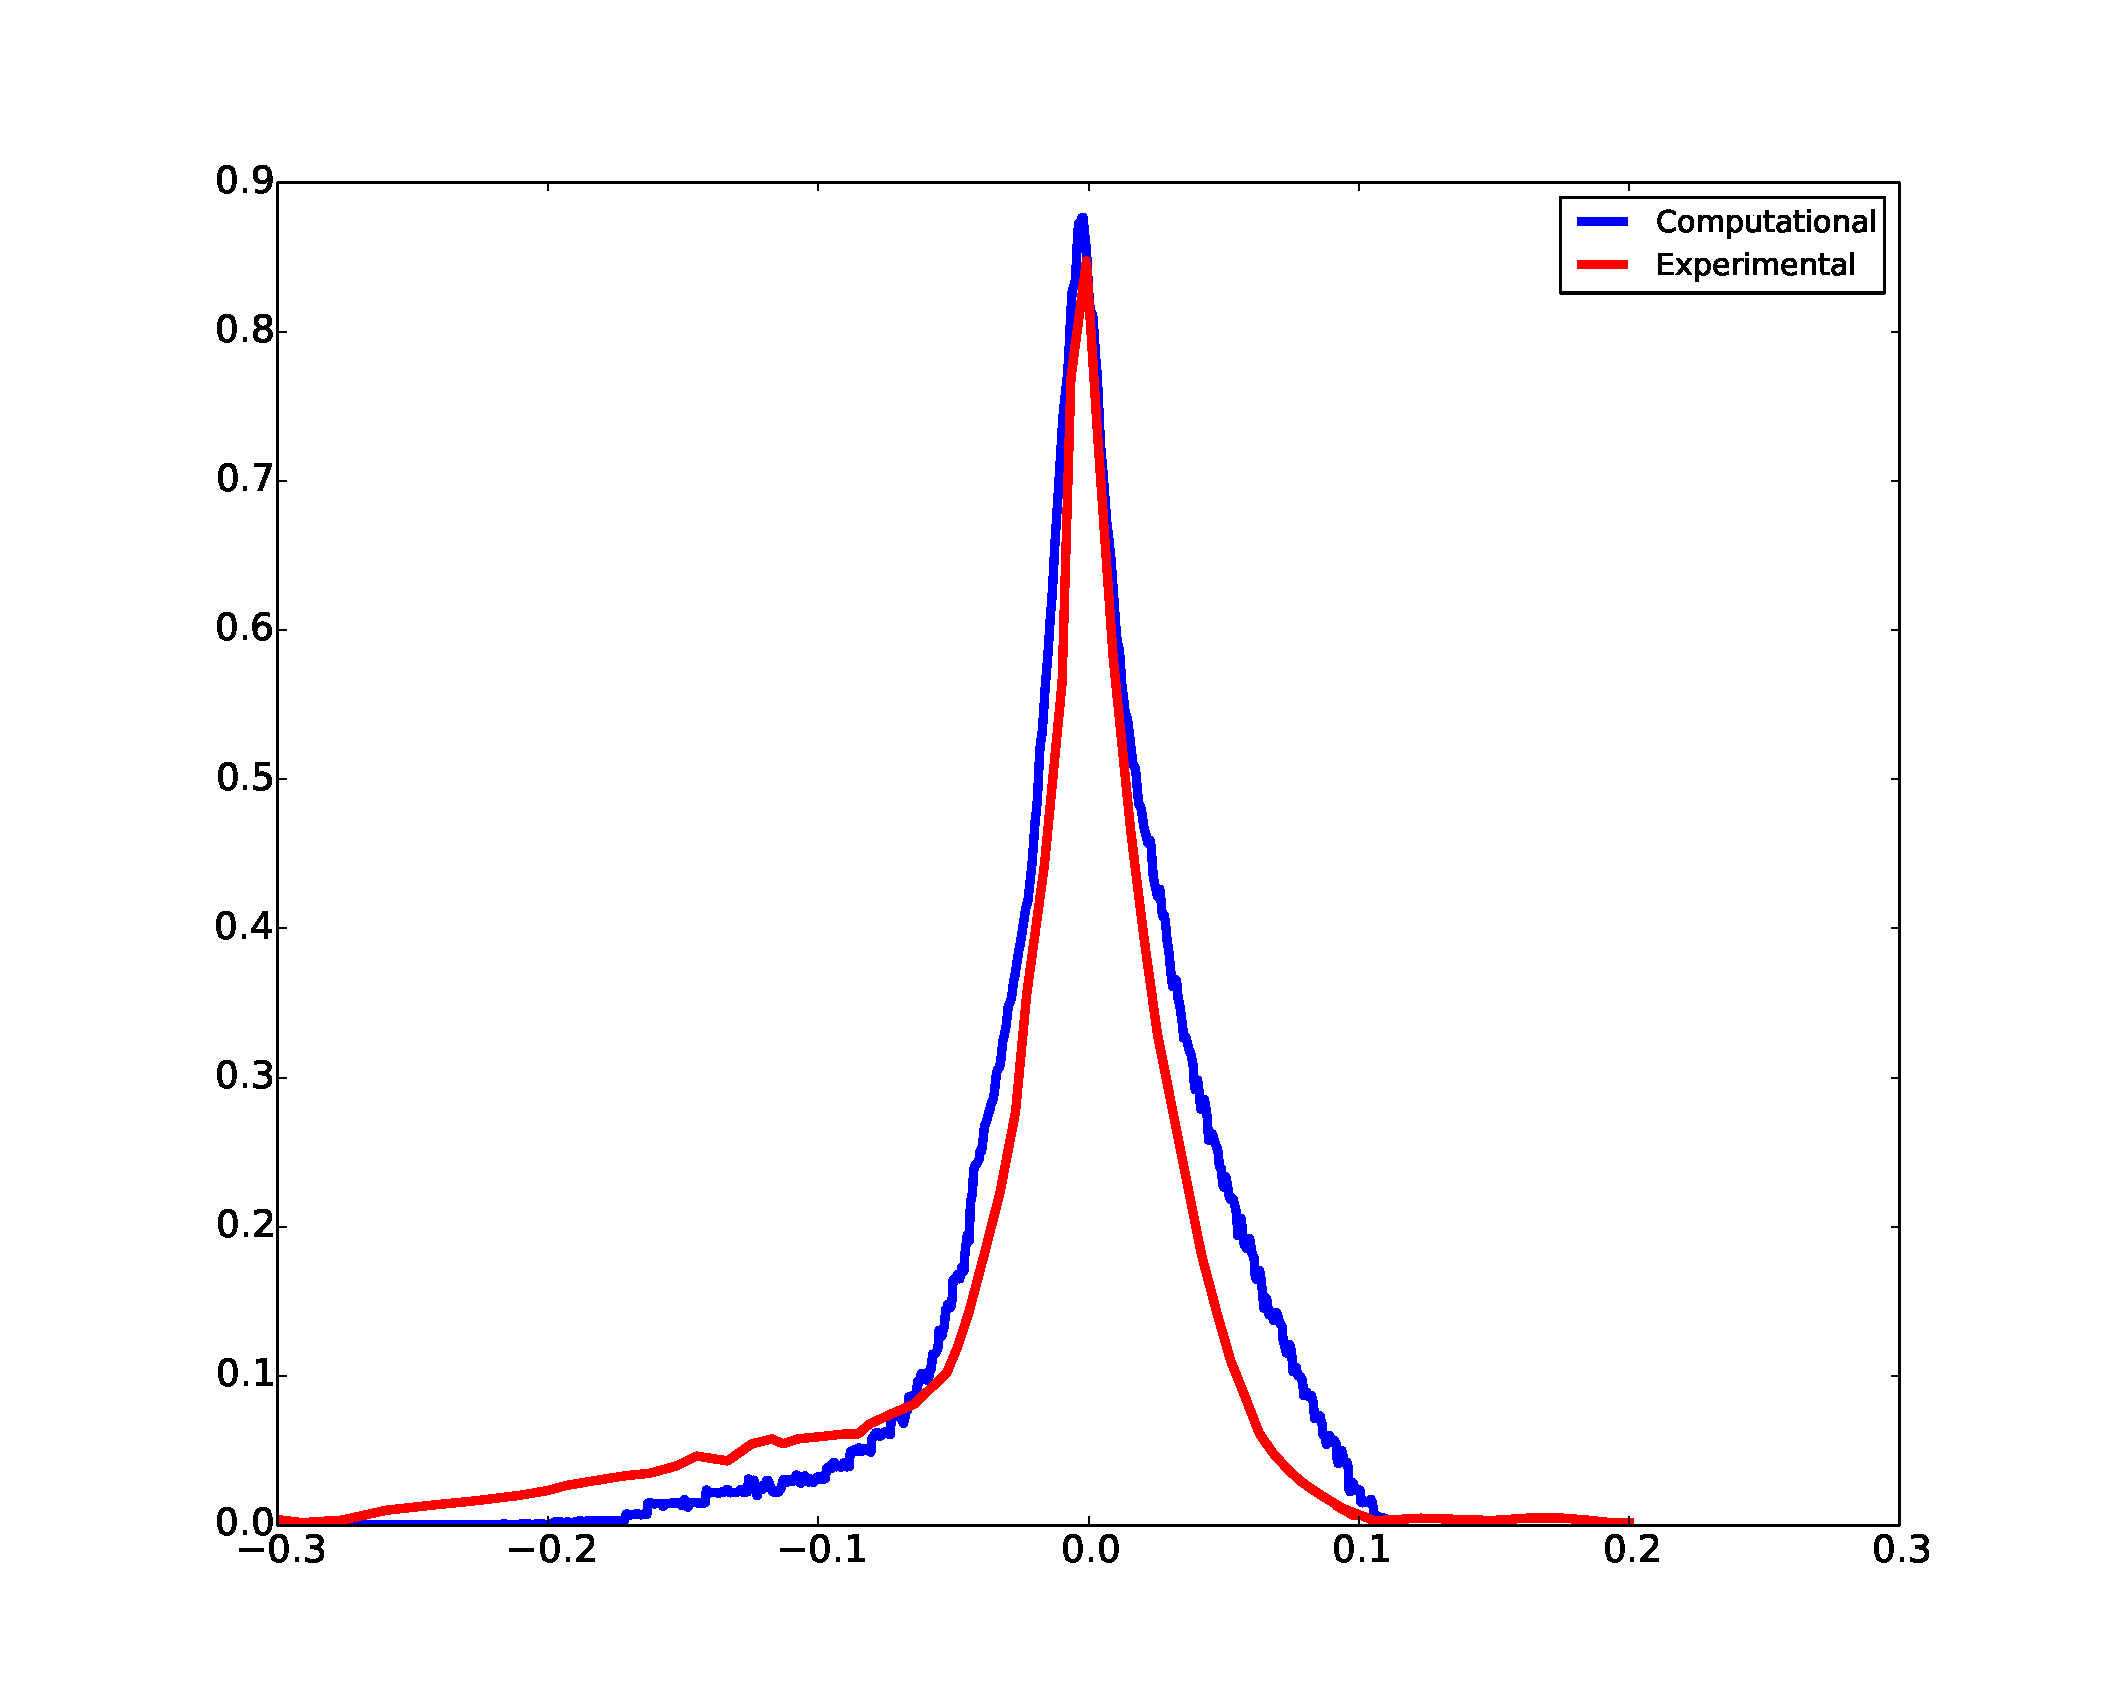
\includegraphics[width=0.65\textwidth]{MVD111} \\
    {\bf MVD 111} \\
    \includegraphics[width=0.65\textwidth]{MVD236} \\
    {\bf MVD 236}
\end{columns}

\begin{itemize}
\item Collection efficiency is the ratio of surface to free-stream water flux
\end{itemize}
\end{frame}
\begin{frame}
\frametitle{Thermodynamics}
\label{sec-5-8}

\begin{equation*}
  \begin{align}
    \rho_w \left \lbrace \frac{\partial h_f}{\partial t} + \nabla \cdot (\bv{u_f} h_f) \right \rbrace &= \dot{m}_{imp} {\color{red} - \dot{m}_{evap}} - \dot{m}_{ice} \\
    \rho_w \left \lbrace \frac{\partial (h_f c_W T)}{\partial t} + \nabla \cdot (\bv{u_f} h_f c_W T) \right \rbrace &= \left [ c_W T_d + \frac{u_d^2}{2} \right ] \dot{m}_{imp} \\
    & {\color{red} -0.5(L_{evap} + L_{sub})\dot{m}_{evap}} \\
    & +(L_{fus} - c_{ice}T)\dot{m}_{ice} \\
    & {\color{red} + \epsilon \sigma (T_{\infty}^4 - T^4)} \\
    & + c_H (T_{\infty} - T)
  \end{align}
\end{equation}

\begin{itemize}
\item \textbf{Mass}
\begin{itemize}
\item Enters through impinging droplets
\item Exits via evaporation/sublimation and freezing
\end{itemize}
\item \textbf{Energy}
\begin{itemize}
\item Enters through impinging droplets, freezing of ice
\item Exits via evaporation/sublimation, radiation, convection
\end{itemize}
\item Solved explicitly using finite volume discretization with Roe scheme upwinding
\end{itemize}
\end{frame}
\begin{frame}
\frametitle{Preliminary Intermediate Results: Ice Shapes}
\label{sec-5-9}

    \centering
    \includegraphics[width=0.65\textwidth]{IceShapeTempSweep}

\begin{itemize}
\item NACA0012, $\alpha = 4^o$, $U_{\infty}$ = 103 m/s, MVD = 20 $\mu m$, LWC = 0.55 g/m$^3$, Re = 4.14 million, T = 7 min
\item Low temperatures: convective heat transfer high enough to freeze all incoming droplets instantly (rime)
\item High temperatures: low amount of ice accretion with liquid film on top (glaze)
\item Intermediate temperatures (glaze/rime mix)
\begin{itemize}
\item Convective heat transfer is minimal at stagnation point and then rises sharply before decaying
\item Results in familiar horn shapes
\end{itemize}
\end{itemize}
\end{frame}
\begin{frame}
\frametitle{Sources of Error}
\label{sec-5-10}

\begin{itemize}
\item \textbf{Convective Heat Transfer}
\begin{itemize}
\item Convective heat transfer calculation is lower than published benchmark test results
\item Habashi,2006 uses rough-wall modification of Spalart-Almaras turbulence model (specifically developed for icing applications)
\item Ice shapes are very sensitive to heat transfer by convection
\end{itemize}
\end{itemize}
    \centering
    \includegraphics[width=0.65\textwidth]{HeatTransferComparison}
\begin{itemize}
\item \textbf{Neglected Thermodynamic Mechanisms}
\begin{itemize}
\item Neglected mass/energy transfer via evaporation/sublimation and radiation
\end{itemize}
\end{itemize}
\end{frame}
\begin{frame}
\frametitle{Work In-Progress}
\label{sec-5-11}

\begin{itemize}
\item Implement rough-wall extension in Spalart-Almaras turbulence model
\item Implement neglected mass/energy transfer mechanisms
\item Verify icing calculations against published results
\item Perform UQ studies, investigate sensitivity to physical parameters
\begin{itemize}
\item Temperature, convective heat transfer coefficient, Reynolds number, MVD, LWC, angle of attack, etc.
\end{itemize}
\end{itemize}
\end{frame}
\begin{frame}
\frametitle{Conclusions/Future Work}
\label{sec-5-12}


\textbf{Conclusions}
\begin{itemize}
\item Airfoil icing is a process subject to much uncertainty
\begin{itemize}
\item Wide variation in ice shapes
\item Sensitivity to perturbations in physical conditions
\end{itemize}
\item We have briefly demonstrated three approaches to quantifying
  uncertainty in this problem
\begin{itemize}
\item Heuristic parameterization
\item Data-based parameterization
\item Computational-based UQ
\end{itemize}
\end{itemize}
\textbf{Future Work}
\begin{itemize}
\item Parameterized UQ
\begin{itemize}
\item Investigate effect of more shape parameters
\item Extend efforts to 3D wing icing
\end{itemize}
\item Computational modeling
\begin{itemize}
\item Continue development and testing of icing code
\item Use icing code to investigate statistical variation of ice shape
\end{itemize}
\end{itemize}
\end{frame}

\end{document}
